\documentclass[tesi]{subfiles}

\IfEq{\jobname}{\detokenize{tesi}}{}{%
	\externaldocument{Chapter1}
    \externaldocument{Chapter4}
}
\begin{document}

\chapter{Road Surface Analysis}
\label{ch:System Development}
This chapter describes the techniques that have been used, focusing on the following topics:

\begin{itemize}
\item How data are collected.
\item Preprocessing and surface condition indexes computation.
\item Storage and Integration of processed data.
\item Indexes visualization on a map.
\end{itemize}

The figure below shows the structure of the system.
\begin{figure}[H]
\centering
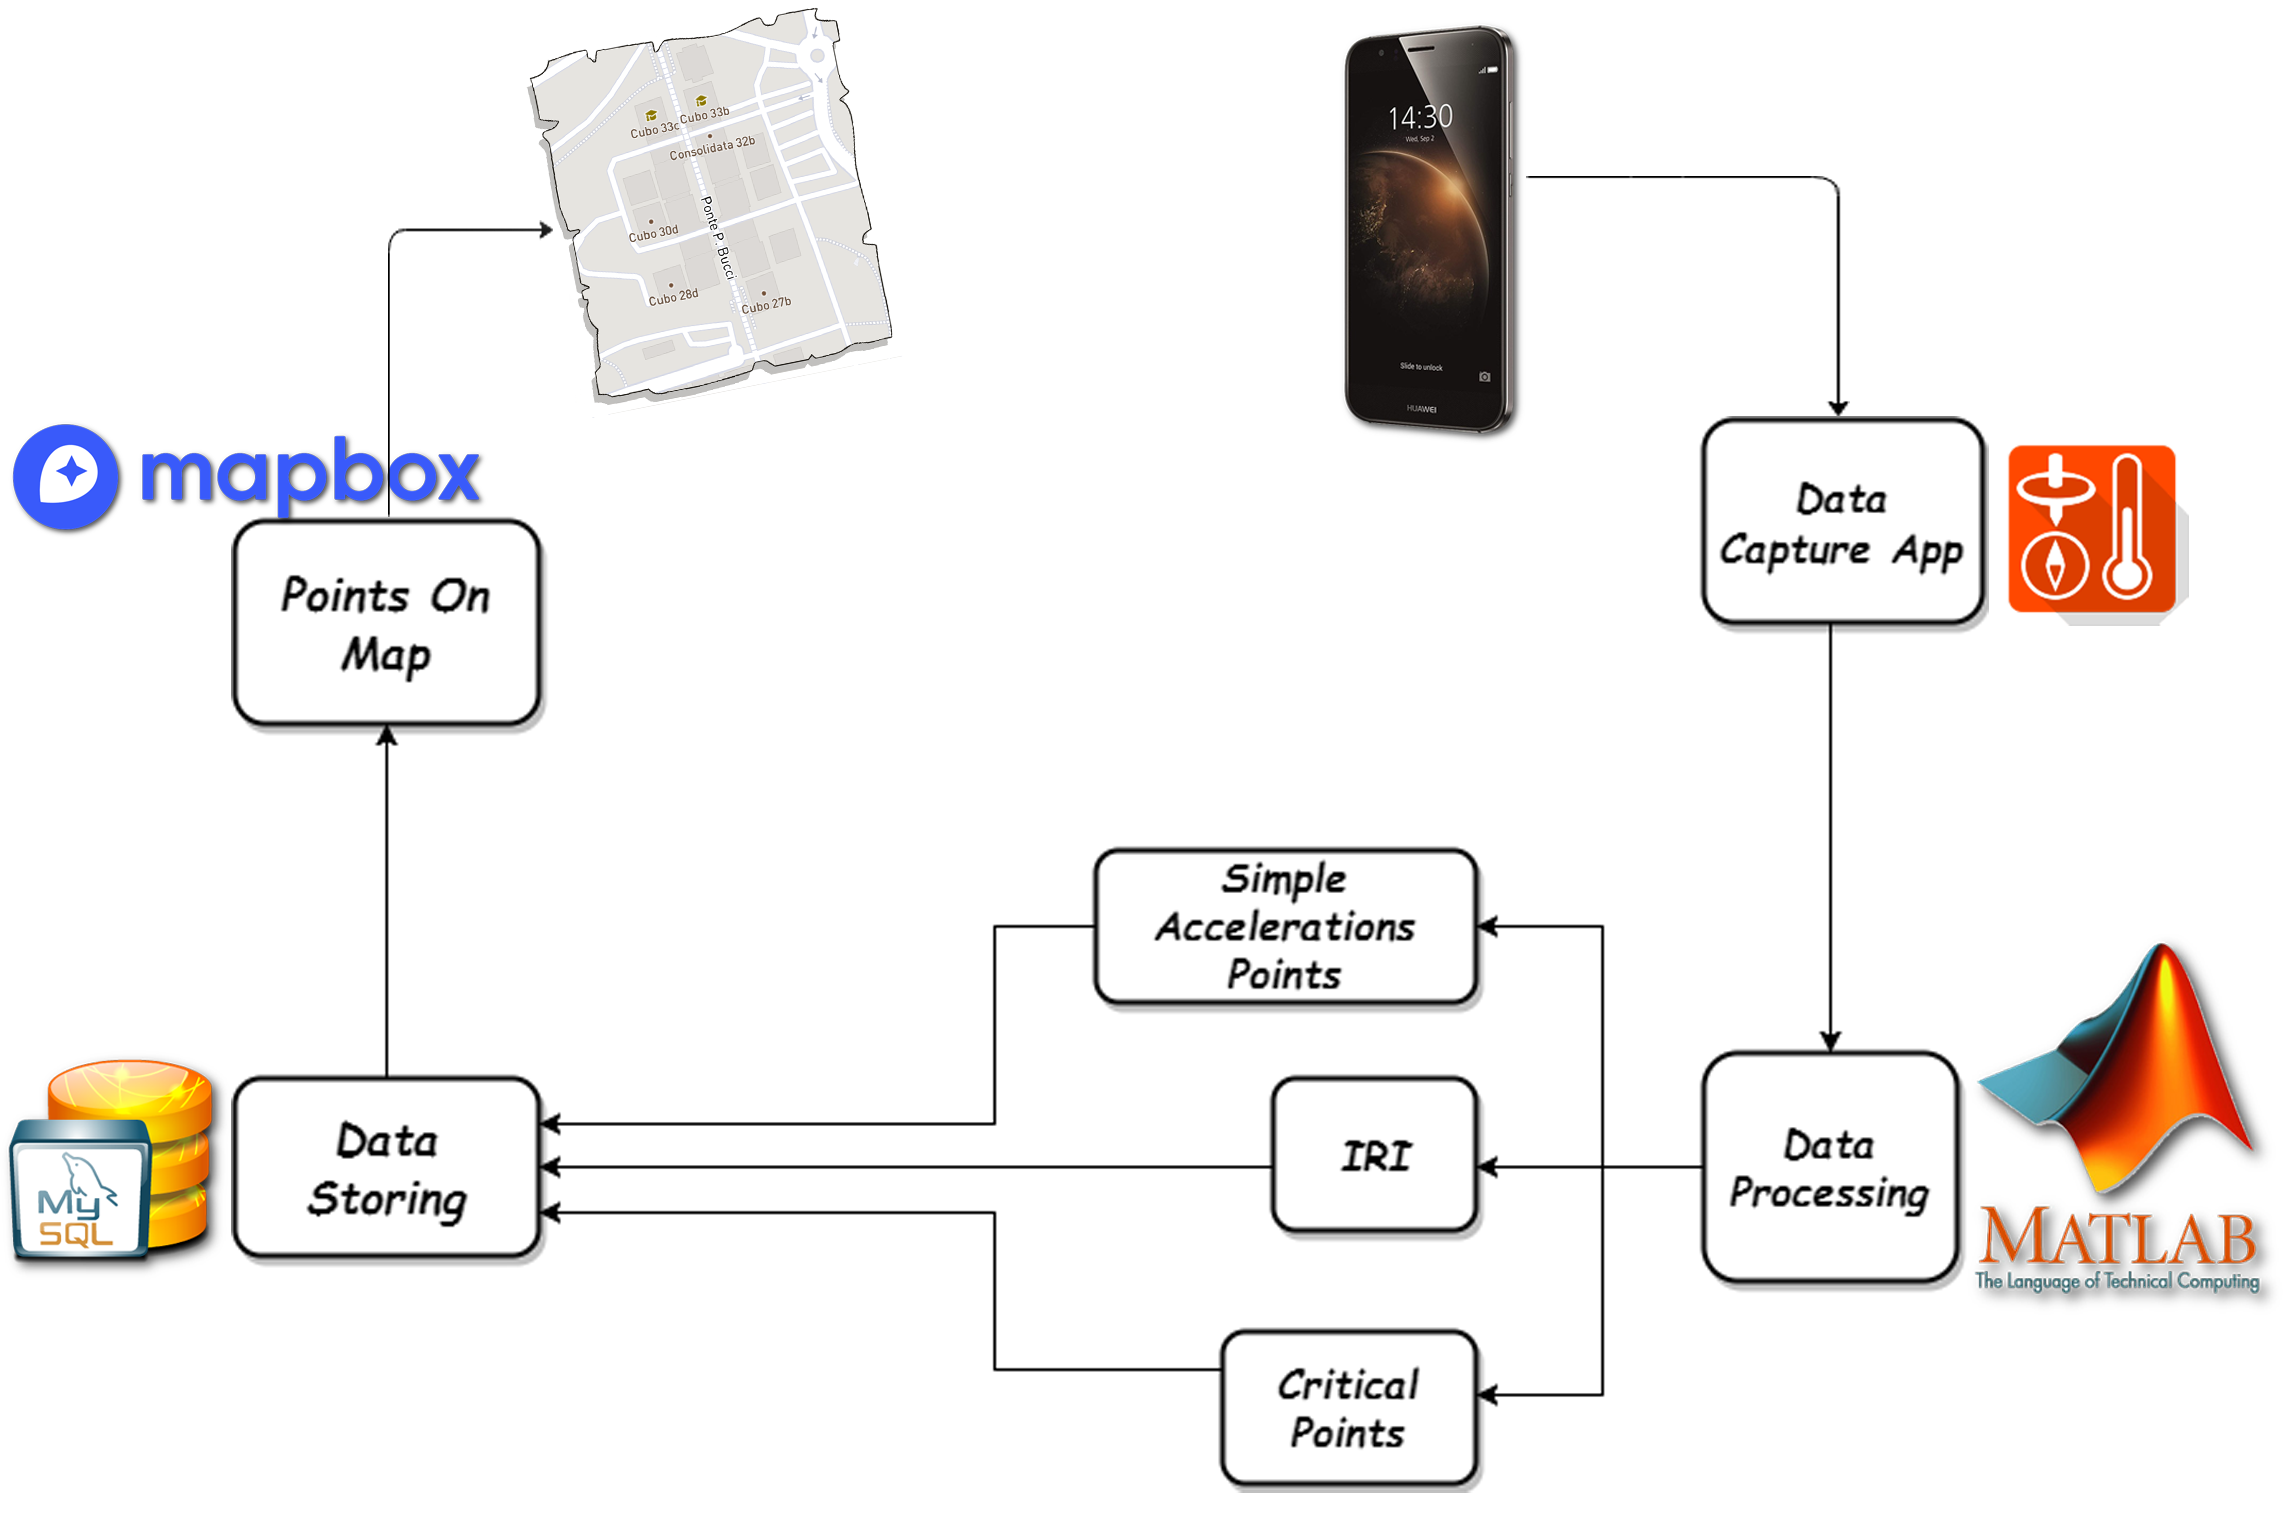
\includegraphics[scale=0.6]{WorkFlow}
\caption{System Structure}

\end{figure}\label{fig:System Structure}

\section{Data Collection}\label{sc:Data Collect}
Initially, the smartphone was fixed up at the windshield of the car by an arm support, forming a $90$-degree angle between the phone and the vehicle axes.
However, during travel, the support was subject to vibrations that caused additional noise in the data, and could also be subject to movements due to the nature of the support itself and the road surface conditions, thus changing the integrity of the data.
The smartphone was then mounted horizontally on the car dashboard, forming a proximal $0$-degree angle with it, using a non-slip material. This setting was optimal because the perceived vibrations by the sensor are proportional to the vibrations experienced by the car's chassis, meaning that the movements of the smartphone itself were sufficiently small.
The \texttt{AndroSensors} application available on the PlayStore was adopted as software for interacting with the sensors. That allows us  performing multiple concurrent measurements of various sensors.

\begin{figure}[H]
 \centering

  \subfloat[Side view]{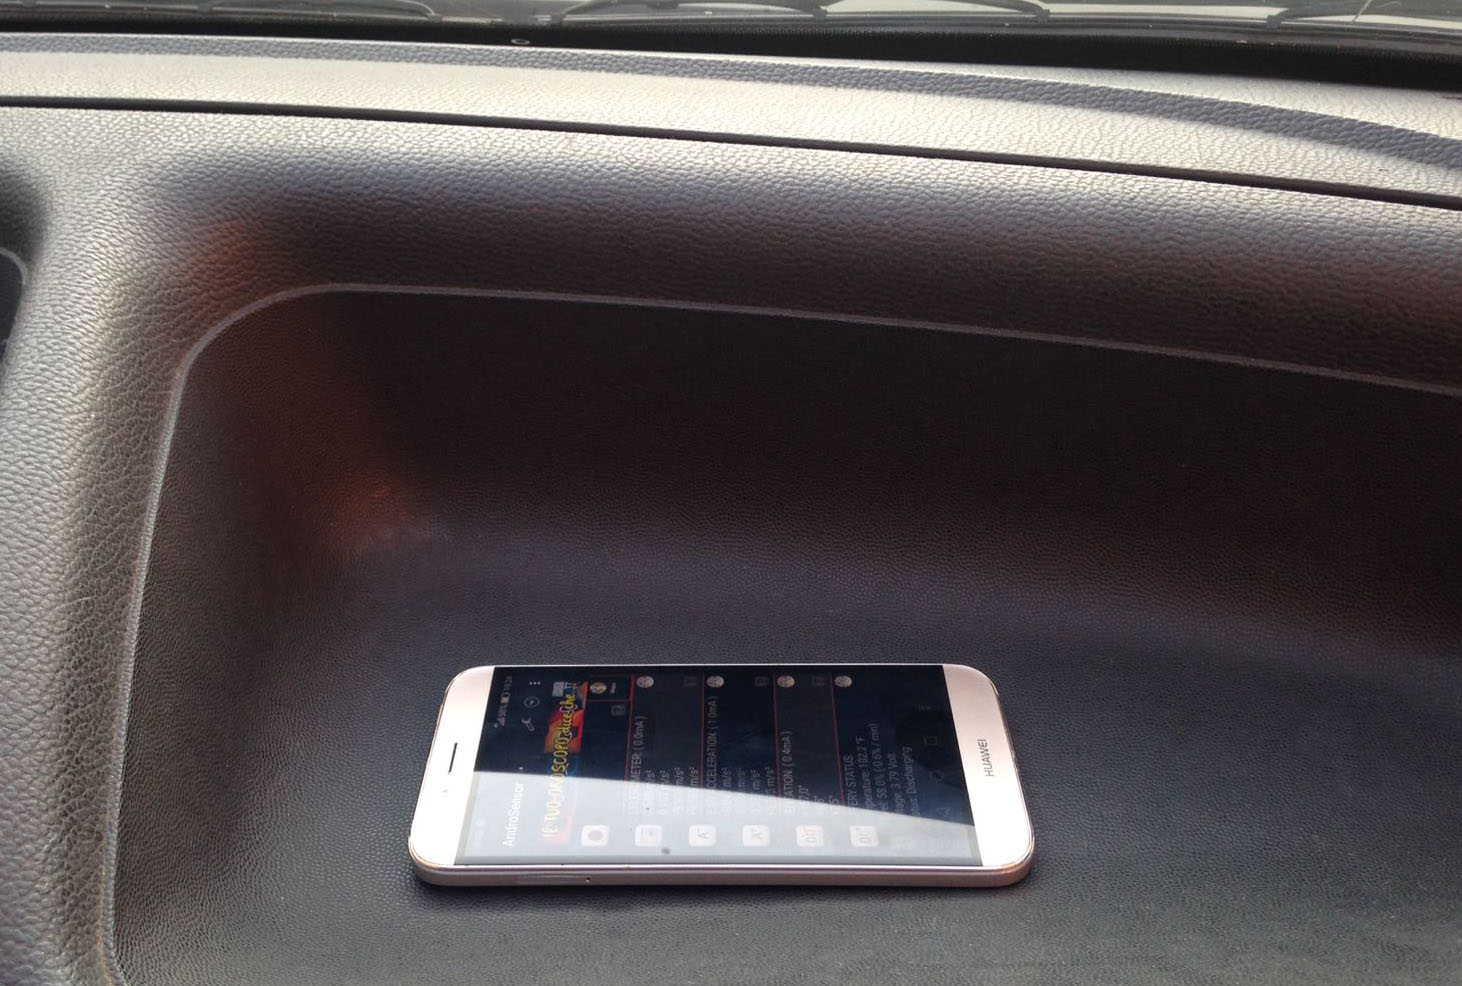
\includegraphics[scale=0.22]{Smartphone2}}
  
  \subfloat[View from above]{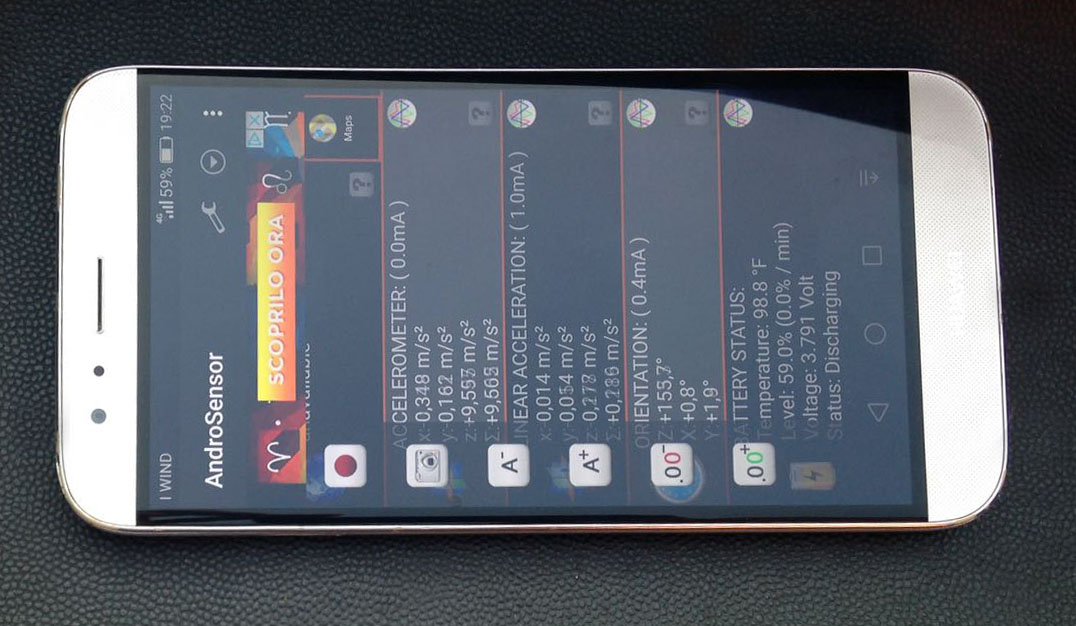
\includegraphics[scale=0.3]{Smartphone1}}
  
  \caption{Smartphone positioning on car dashboard while recording data.}
\end{figure}\label{fig:Smarphone Data Recording}

For out analysis, data was gathered from the following sensors:

\begin{itemize}
\item Accelerometer.
\item Linear Accelerometer.
\item GPS.
\item Orientation.
\item Date
\item Time
\end{itemize}
\clearpage
The data are updated at the highest frequency \textit{"Very Fast"}, while the sampling frequency can be chosen within a range that goes:
\begin{center}
$fs_{min} \quad <= \thinspace f_{s} \thinspace <= \thinspace fs_{max}$\\
$200 \thinspace Hz \quad <= \thinspace f_{s} \thinspace <= \thinspace 1 \thinspace Hz$\\
$0,005 \thinspace s <= \thinspace f_{s} \thinspace <= \thinspace 1 \thinspace s $
\end{center}

Choosing a very low sampling frequency (for example, $fs_{min}$, sensor values may be inconsistent at writing time due to their fast sampling frequency.
However, the higher is the sample rate, the better the final result of our analysis is since it can work on more samples and reduce the overall error.
Conversely, choosing a very high sampling frequency, (for example, $fs_{max}$), we will have very disconnected data, in fact, travelling at a speed of $130 \thinspace \si{\km\per\hour}$, data would be collected every $36,11  \si{\meter}$, which is not favourable to the monitoring of road surface conditions.
Because of these reasons, the sampling frequency was fixed at the following value:
\begin{center}
$fs = 100 \thinspace Hz; \quad fs = 0,01s; \quad fs = 10ms$
\end{center}

Which is stable, and for every second of recording, $100$ samples are collected.
On the adopted hardware, unfortunately, the GPS sensors cannot sample at frequencies lower than $1 \thinspace Hz$ (there are smartphones that are capable of reaching $20 \thinspace Hz$).
Once the GPS signal has been established, it is possible to start recording the data.



 \section{Data Processing}\label{sc:Data Processing}
 Regarding data processing, 3 indexes will be extrapolated:

 \begin{itemize}
 \item Simple Accelerations Points
 \item Critical Points
 \item IRI
 \end{itemize}
 
Once the measurements are complete, the data will be saved in a $.xls$ file.
These will be processed with MATLAB (Matrix Laboratory) a multi-paradigm numerical computing environment, which makes numerical computing more easier and computationally faster than other programming paradigms.
Initially, the $.xls$ file is read, and each column of it depending on the data nature (numeric or string) will be stored in a vector, which can be found in the MATLAB workspace.
Once the raw data has been read, the indexes computation starts.

\clearpage
\subsection{Simple Acceleration Points}\label{ssc:Simple Accelerations Points}
This index helps principally to show how the acceleration component changes depending on different points on the road surface.
It notes that an appropriate methodology is needed to calculate the surface conditions because the representation of the acceleration signal alone would not be satisfactory to provide all the conditions of a given road segment. This index will be calculated on a segment of a predetermined length ($distance_{segment}$, from now it is called $ds$) in which an $\chi$ value will be associated and calculated as follows:

\begin{center}
{\large  $\chi \thinspace = \left( \sum \limits_{i=1}^{N} \thinspace a_{i} \right) \thinspace \dfrac{1}{N}$}
\end{center}\label{eq:sap}
where:
\begin{itemize}
\item $N$ is the number of GPS points necessary to reach a lenght of $ds$
\item $a_{i}$ is the processed acceleration value associated to $i$
\end{itemize}

For example, considering a urban road in good conditions, the travel speed is low, so for each considered segment, the number of samples collected per second is high.
This means that the final result is obtained averaging many points.
High energy peaks are smoothed by low energy samples by which are outnumbered.
The end result will definitely have a small value.
This value would indicate that the condition of the road surface it is almost perfect, although it might not be the case.
On the other hand, when taking into consideration an highway, the travel speed is  high so for each analysed segment, the number of samples available is lower, since the segment is traversed in a shorter amount of time.
High energy peaks are not outnumbered by the low energy peaks so the resulting in a higher computed value, which should suggests that road surface conditions is not optimal.

For each considered segment the proposed indexes is computed performing the following steps:

For example considering the following signal:
\begin{figure}[H]
\centering
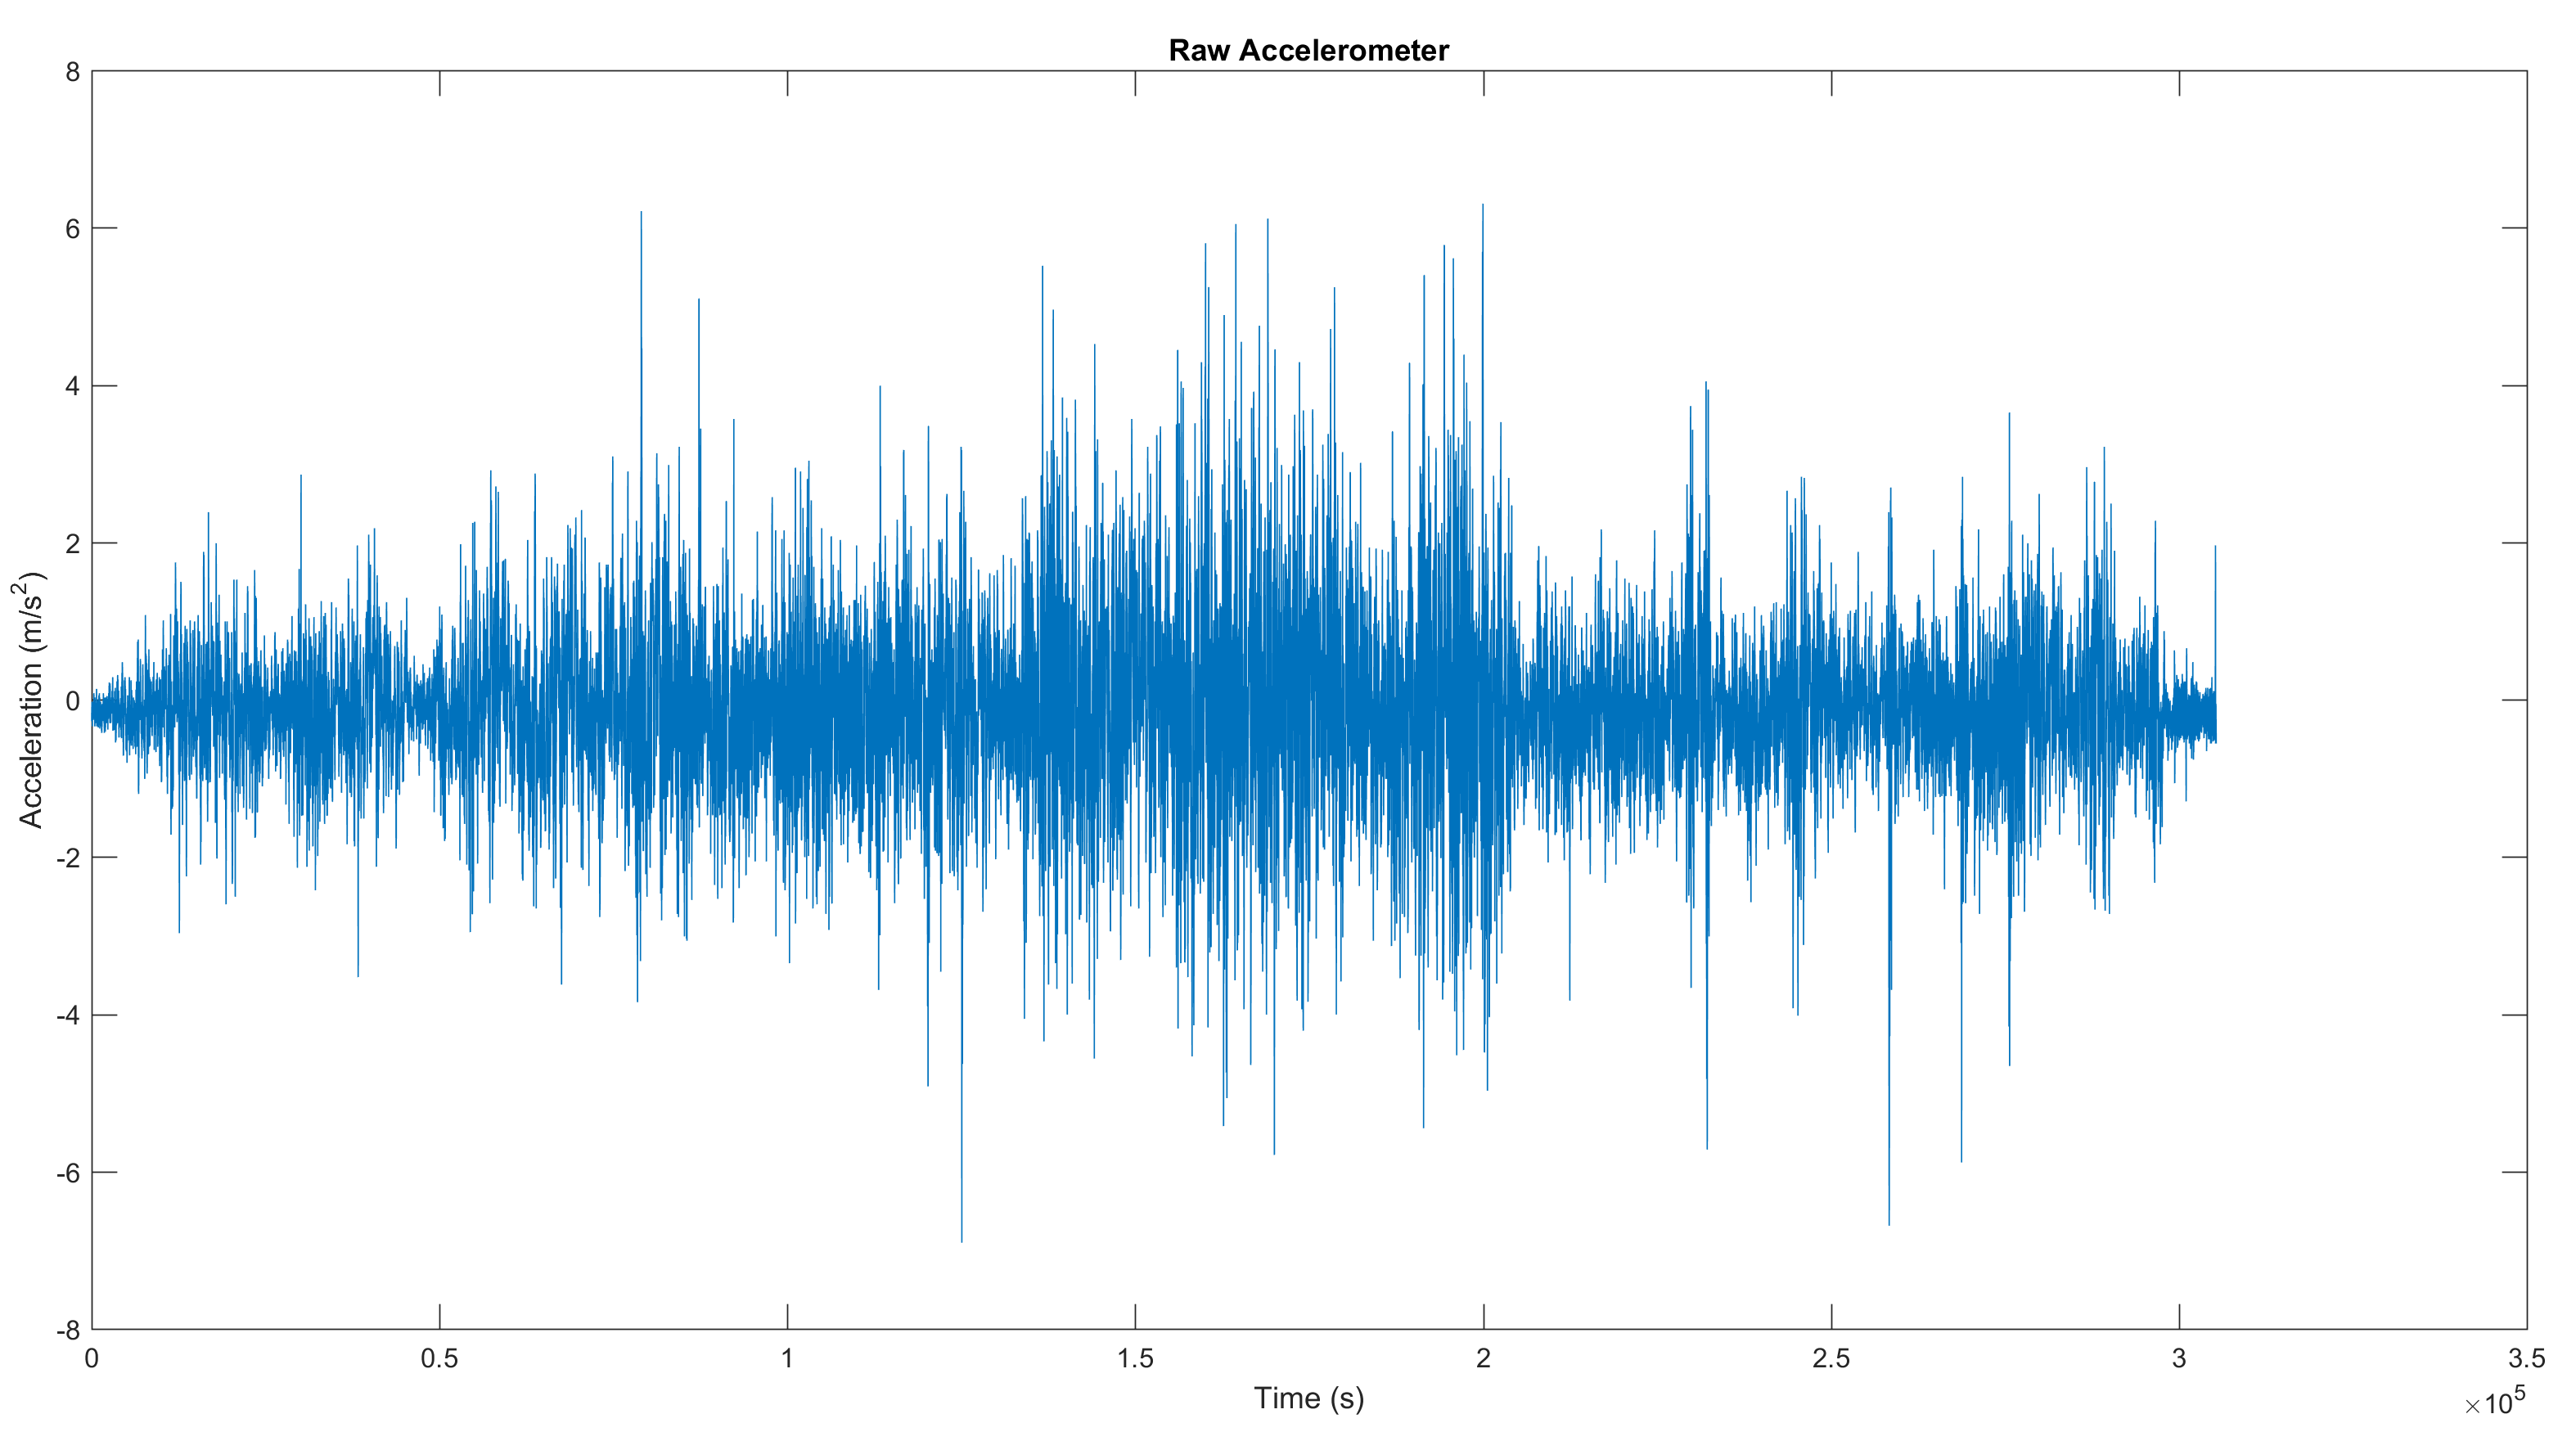
\includegraphics[scale=0.16]{SPARaw}
\caption{Raw Accelerometer Signal}
\end{figure}

The steps are as follows:

\begin{description}
\item[1. Accelerometer Reorientation:] First of all it is applied the procedure of Accelerometer reorientation explained in Chapter\ref{ch:Data Analysis} (section:\ref{sc:Accelerometer Reorientation}, on page: \pageref{sc:Accelerometer Reorientation}).
\item[2. GPS points division:] Next, the GPS points are subdivided according to the methodology explained in Chapter\ref{ch:Data Analysis} (section:\ref{sc:GPS points division}, on page: \pageref{sc:GPS points division}).
\item[3. Filtering Engine Vibrations:] This filter is the first operation that is performed on the data, in which the noise components generated by the engine will be smoothed, according to the application seen in the Chapter\ref{ch:Data Analysis} (section:\ref{sc:Data Filtering}, on a page:\pageref{sssc:Remove Engine Vibrations Filter})

A figure below shows how the filter is applied on the Signal

\begin{figure}[H]
\centering
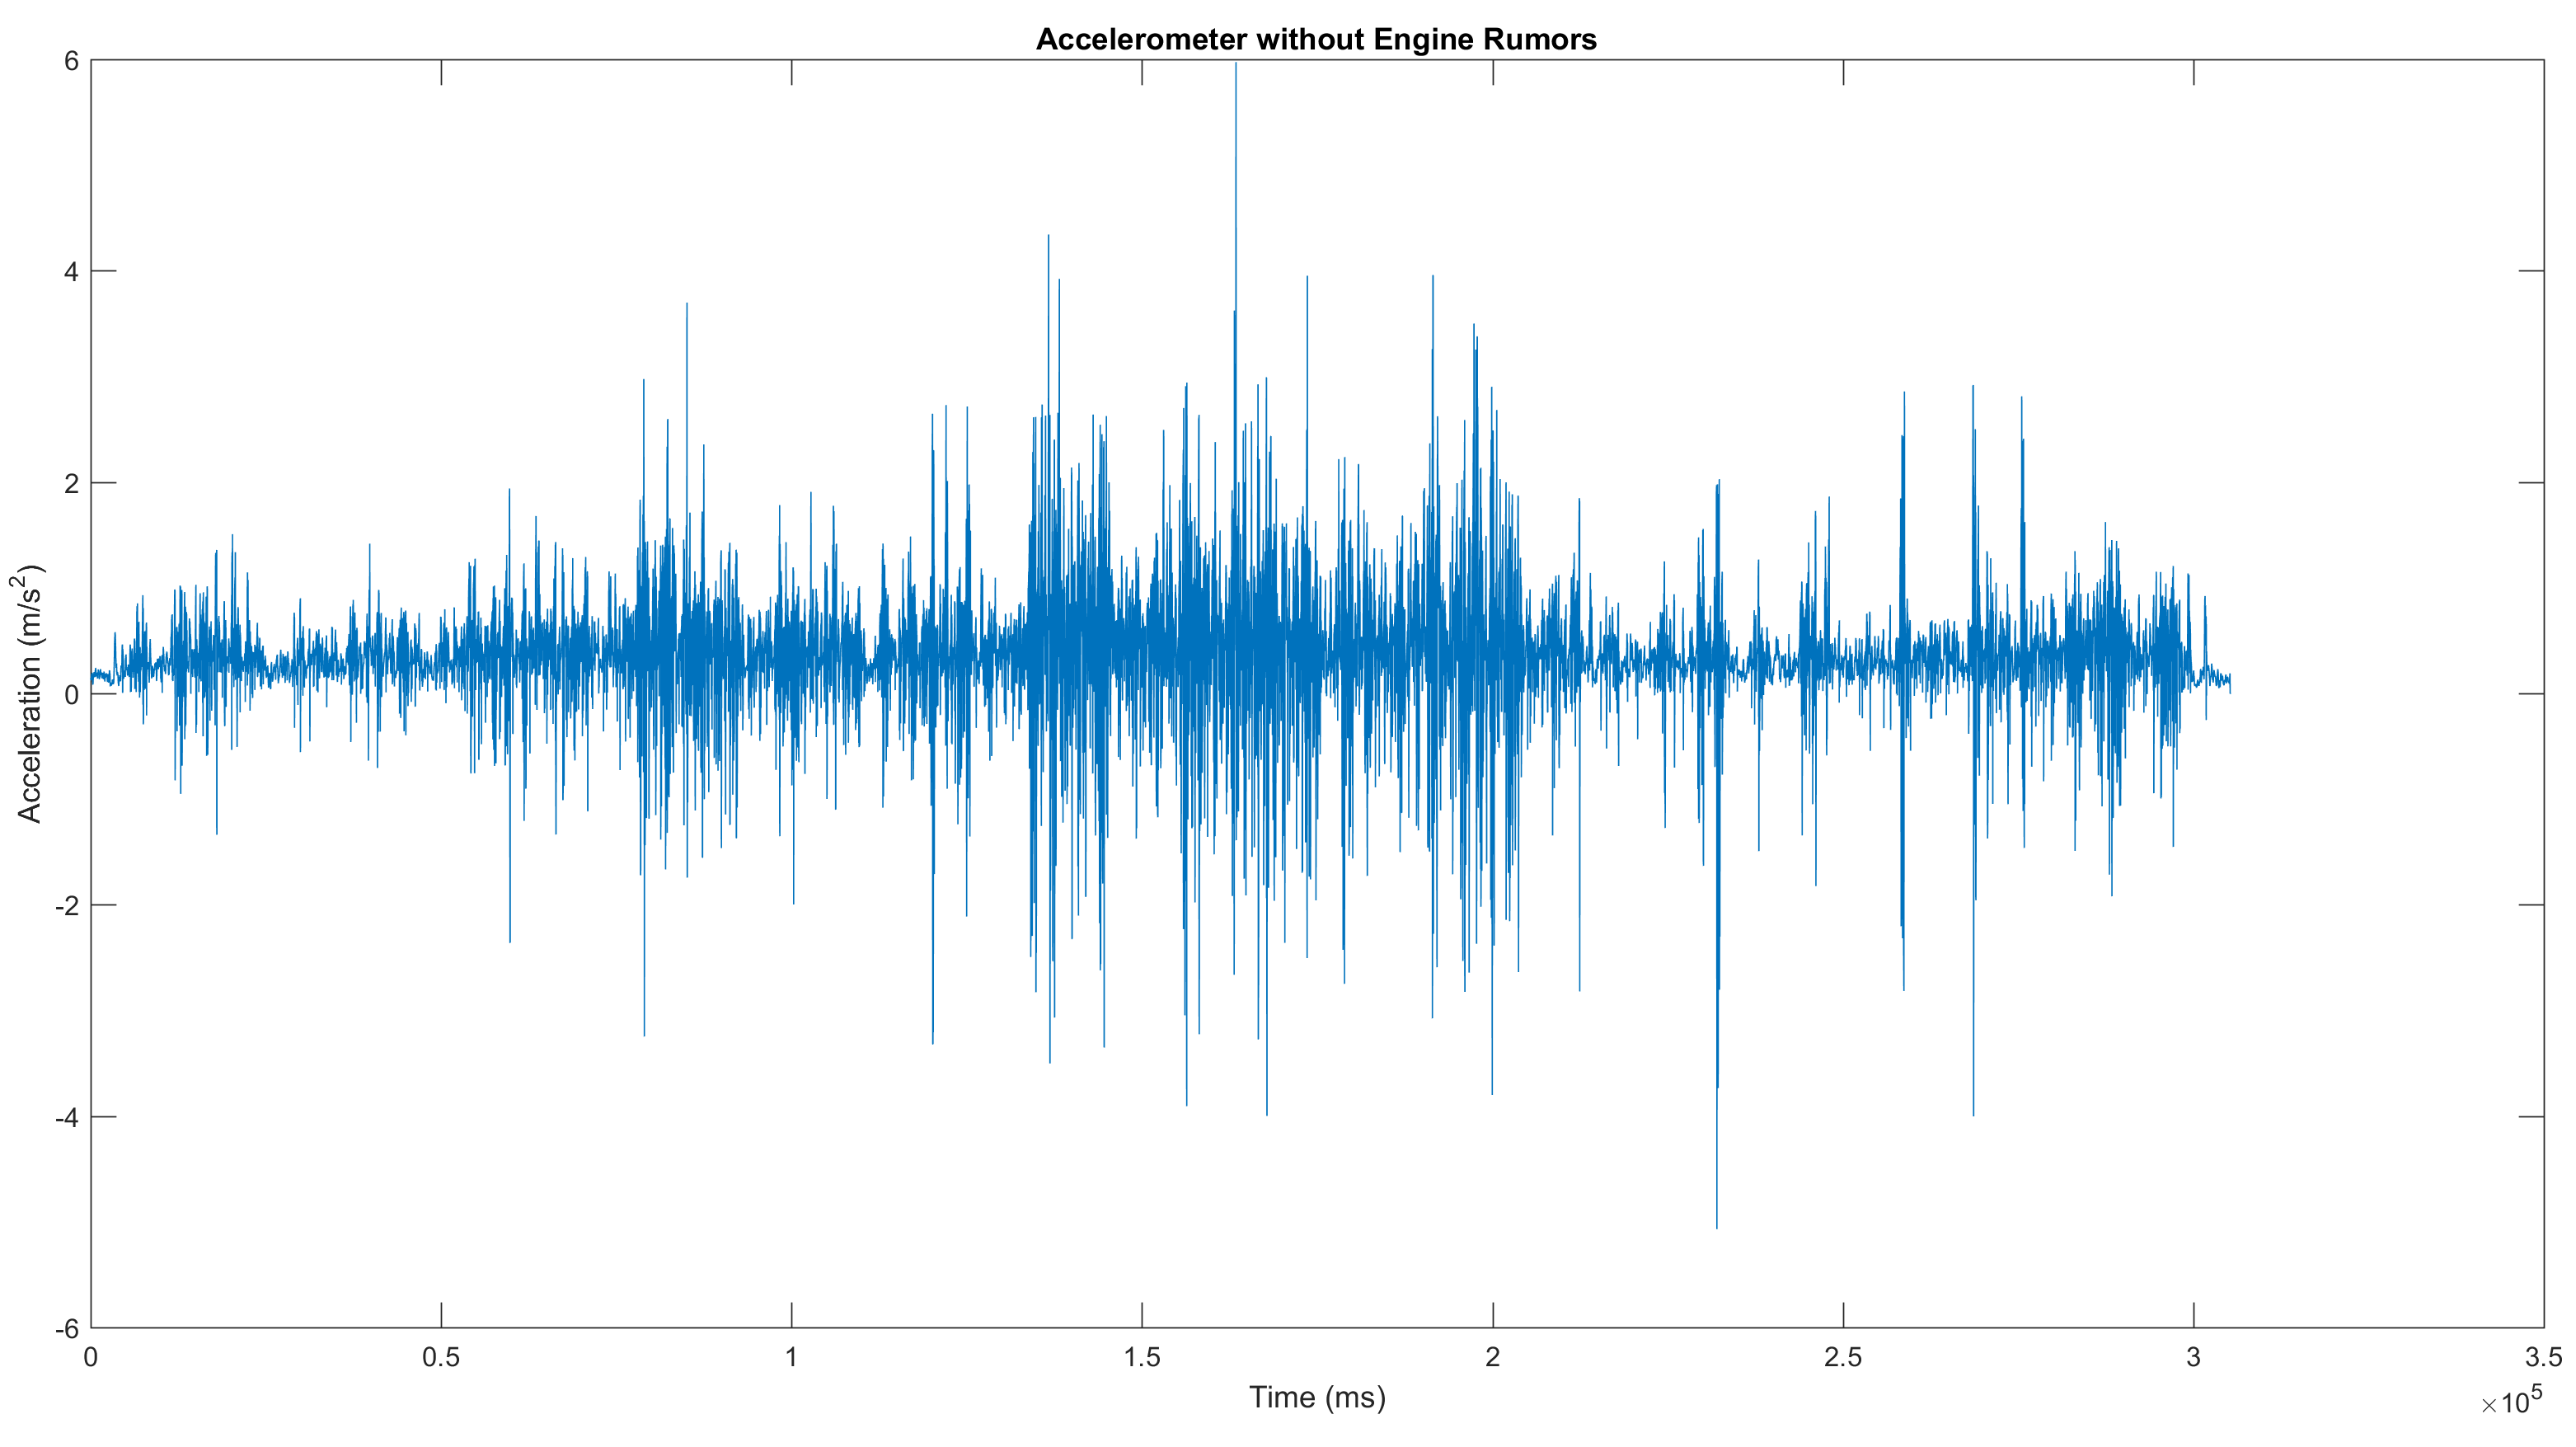
\includegraphics[scale=0.16]{SPANoEngine}
\caption{Signal after application of the filter}
\end{figure}
\item[4. Zero Velocity Filter:] After applying the first filter, this is also applied, as it is explained in the Chapter\ref{ch:Data Analysis} (section:\ref{sc:Data Filtering}, on page:\pageref{sssc:Zero Velocity Filter}).

A figure below shows how the filter is applied on the Signal
\begin{figure}[H]
\centering
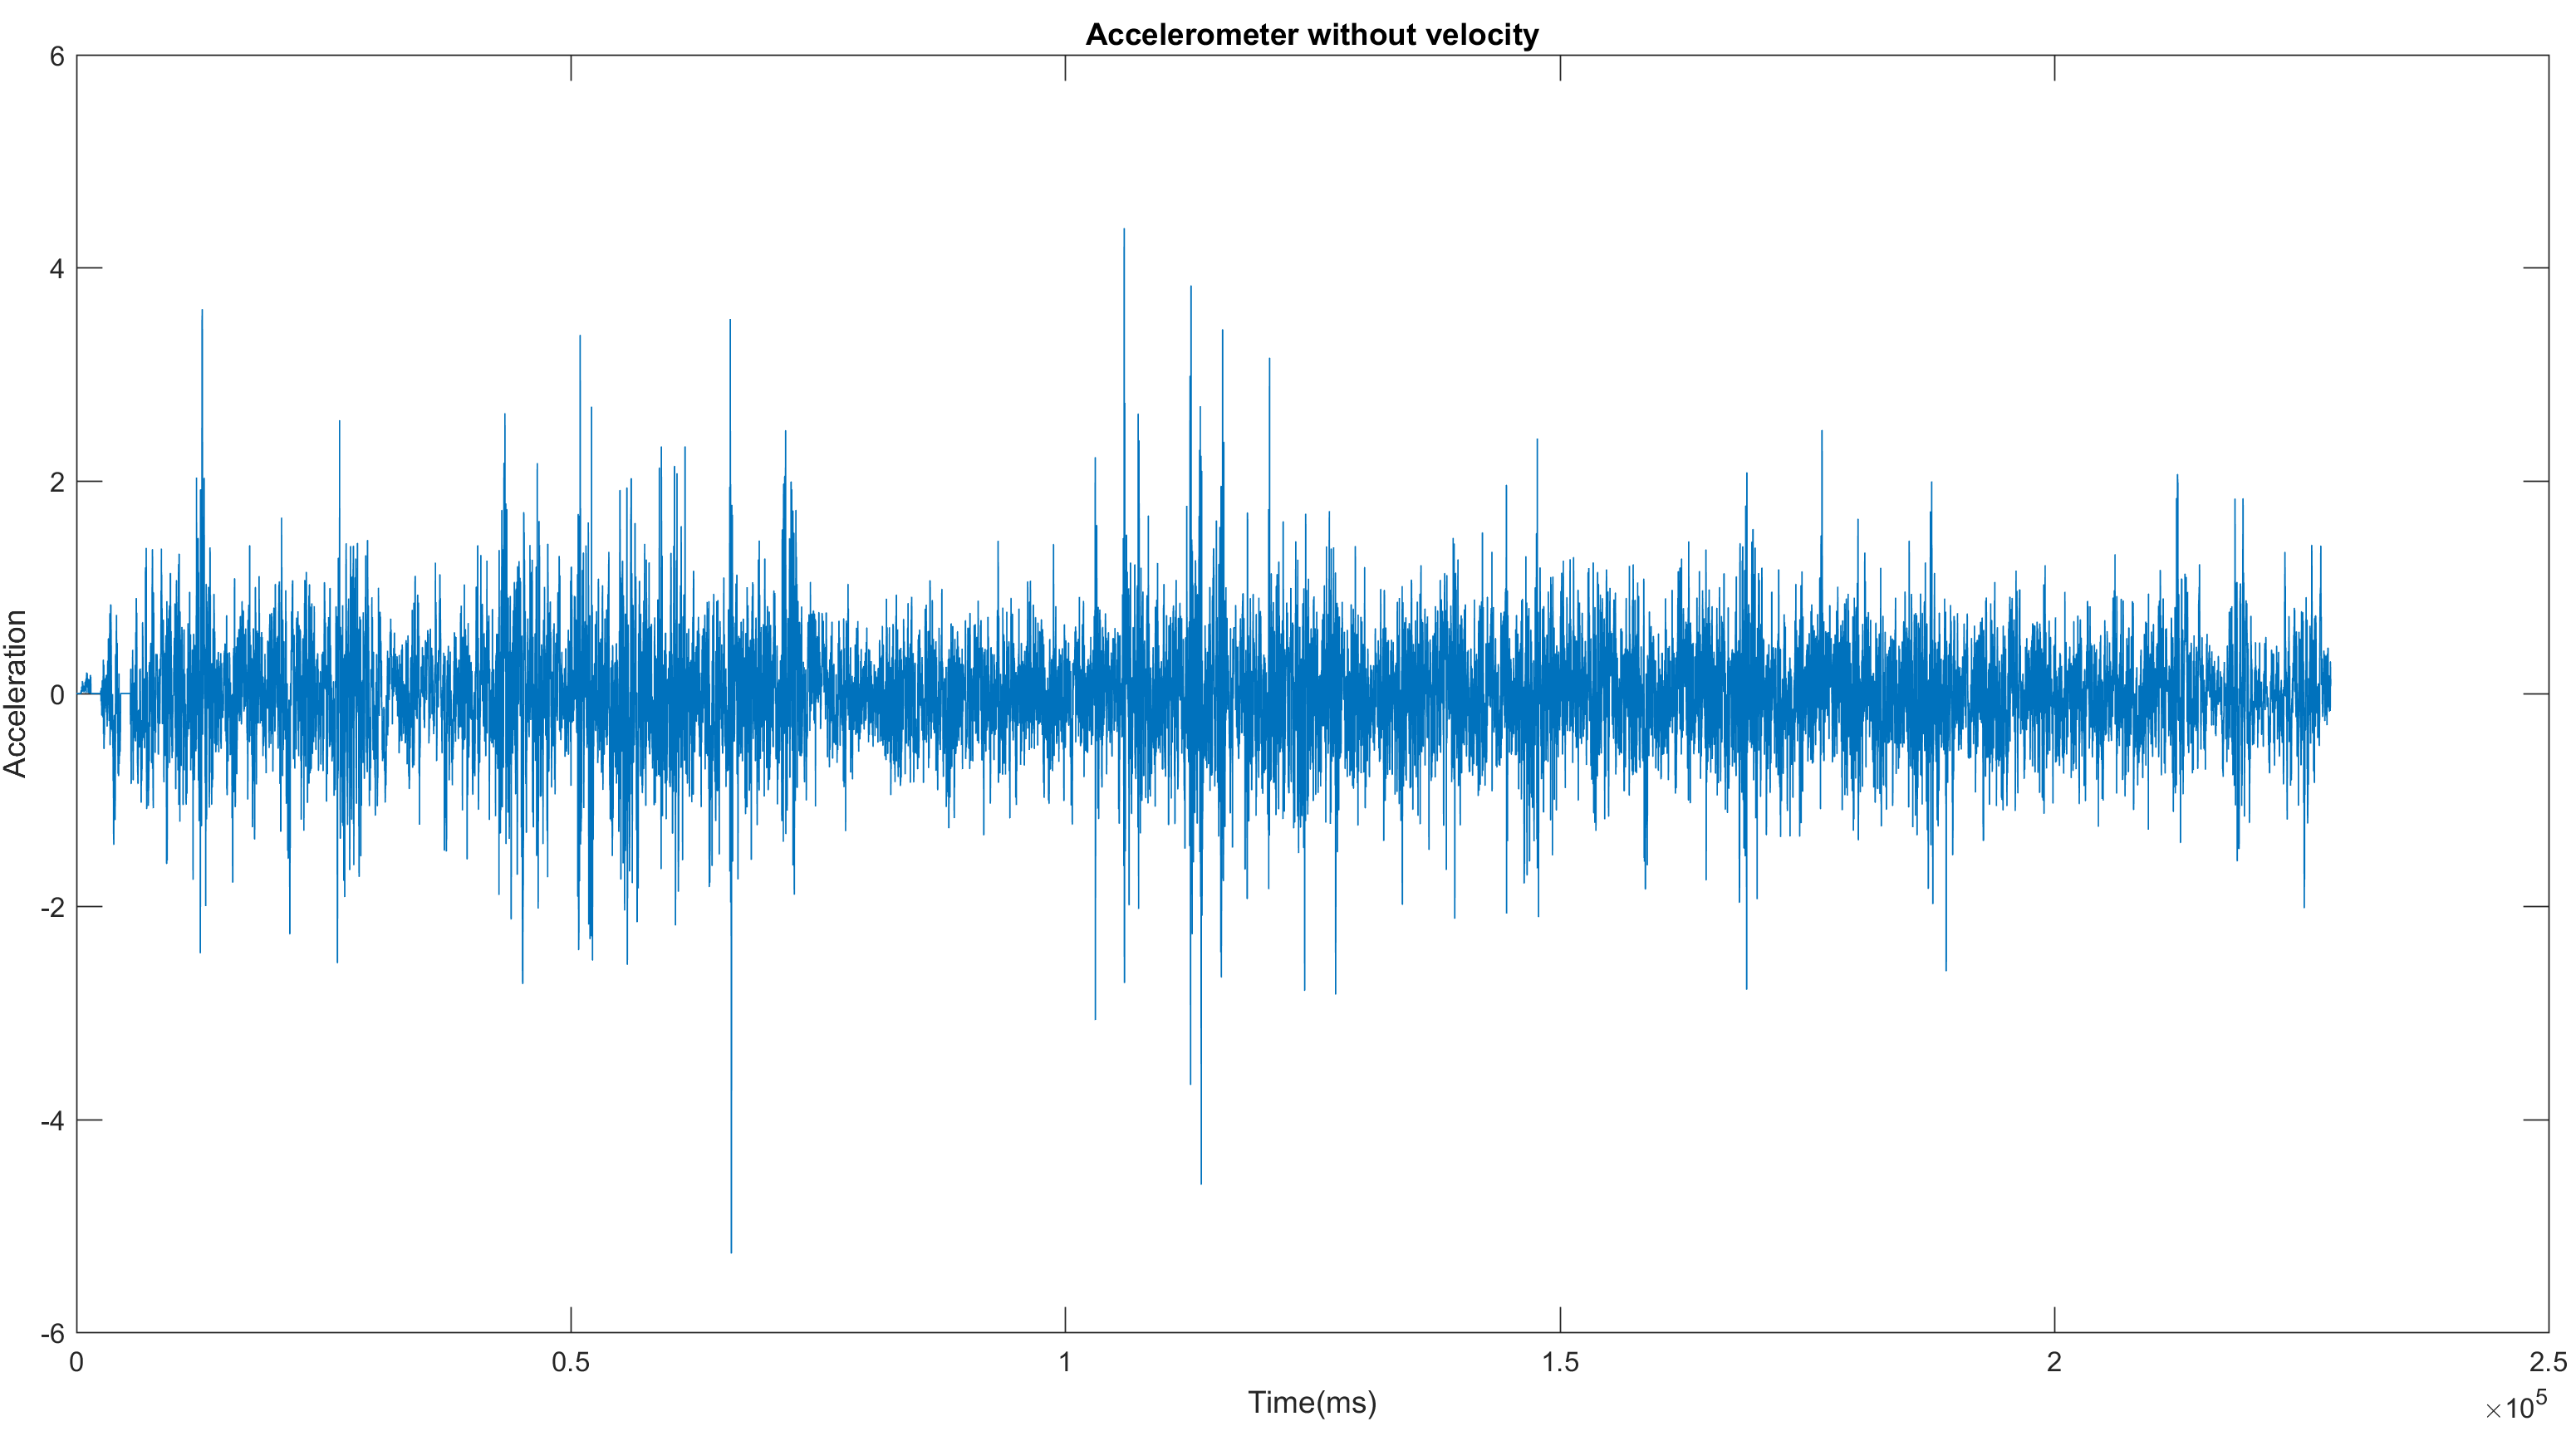
\includegraphics[scale=0.14]{SPANoVelocity}
\caption{Signal after application of the filter}
\end{figure}

\item[5. Calculation of the final index:] Ultimately, the final index is calculated.
This value it is associated with a certain portion of the road ($ds$). Following the application of the two previous filters, the Haversine formula will be used (as it is explained on a page: \ref{ssc:Haversine Formula}) to calculate the cumulative GPS distance of points until the $ds$ is reached. The new GPS point will be identified by the set of points needed to compose the segment. For the $\chi$ \thinspace \ref{eq:sap} value, it will be calculated by all the acceleration values that are simultaneously read together with GPS points.

A figure below show the result.
\begin{figure}[H]
\centering
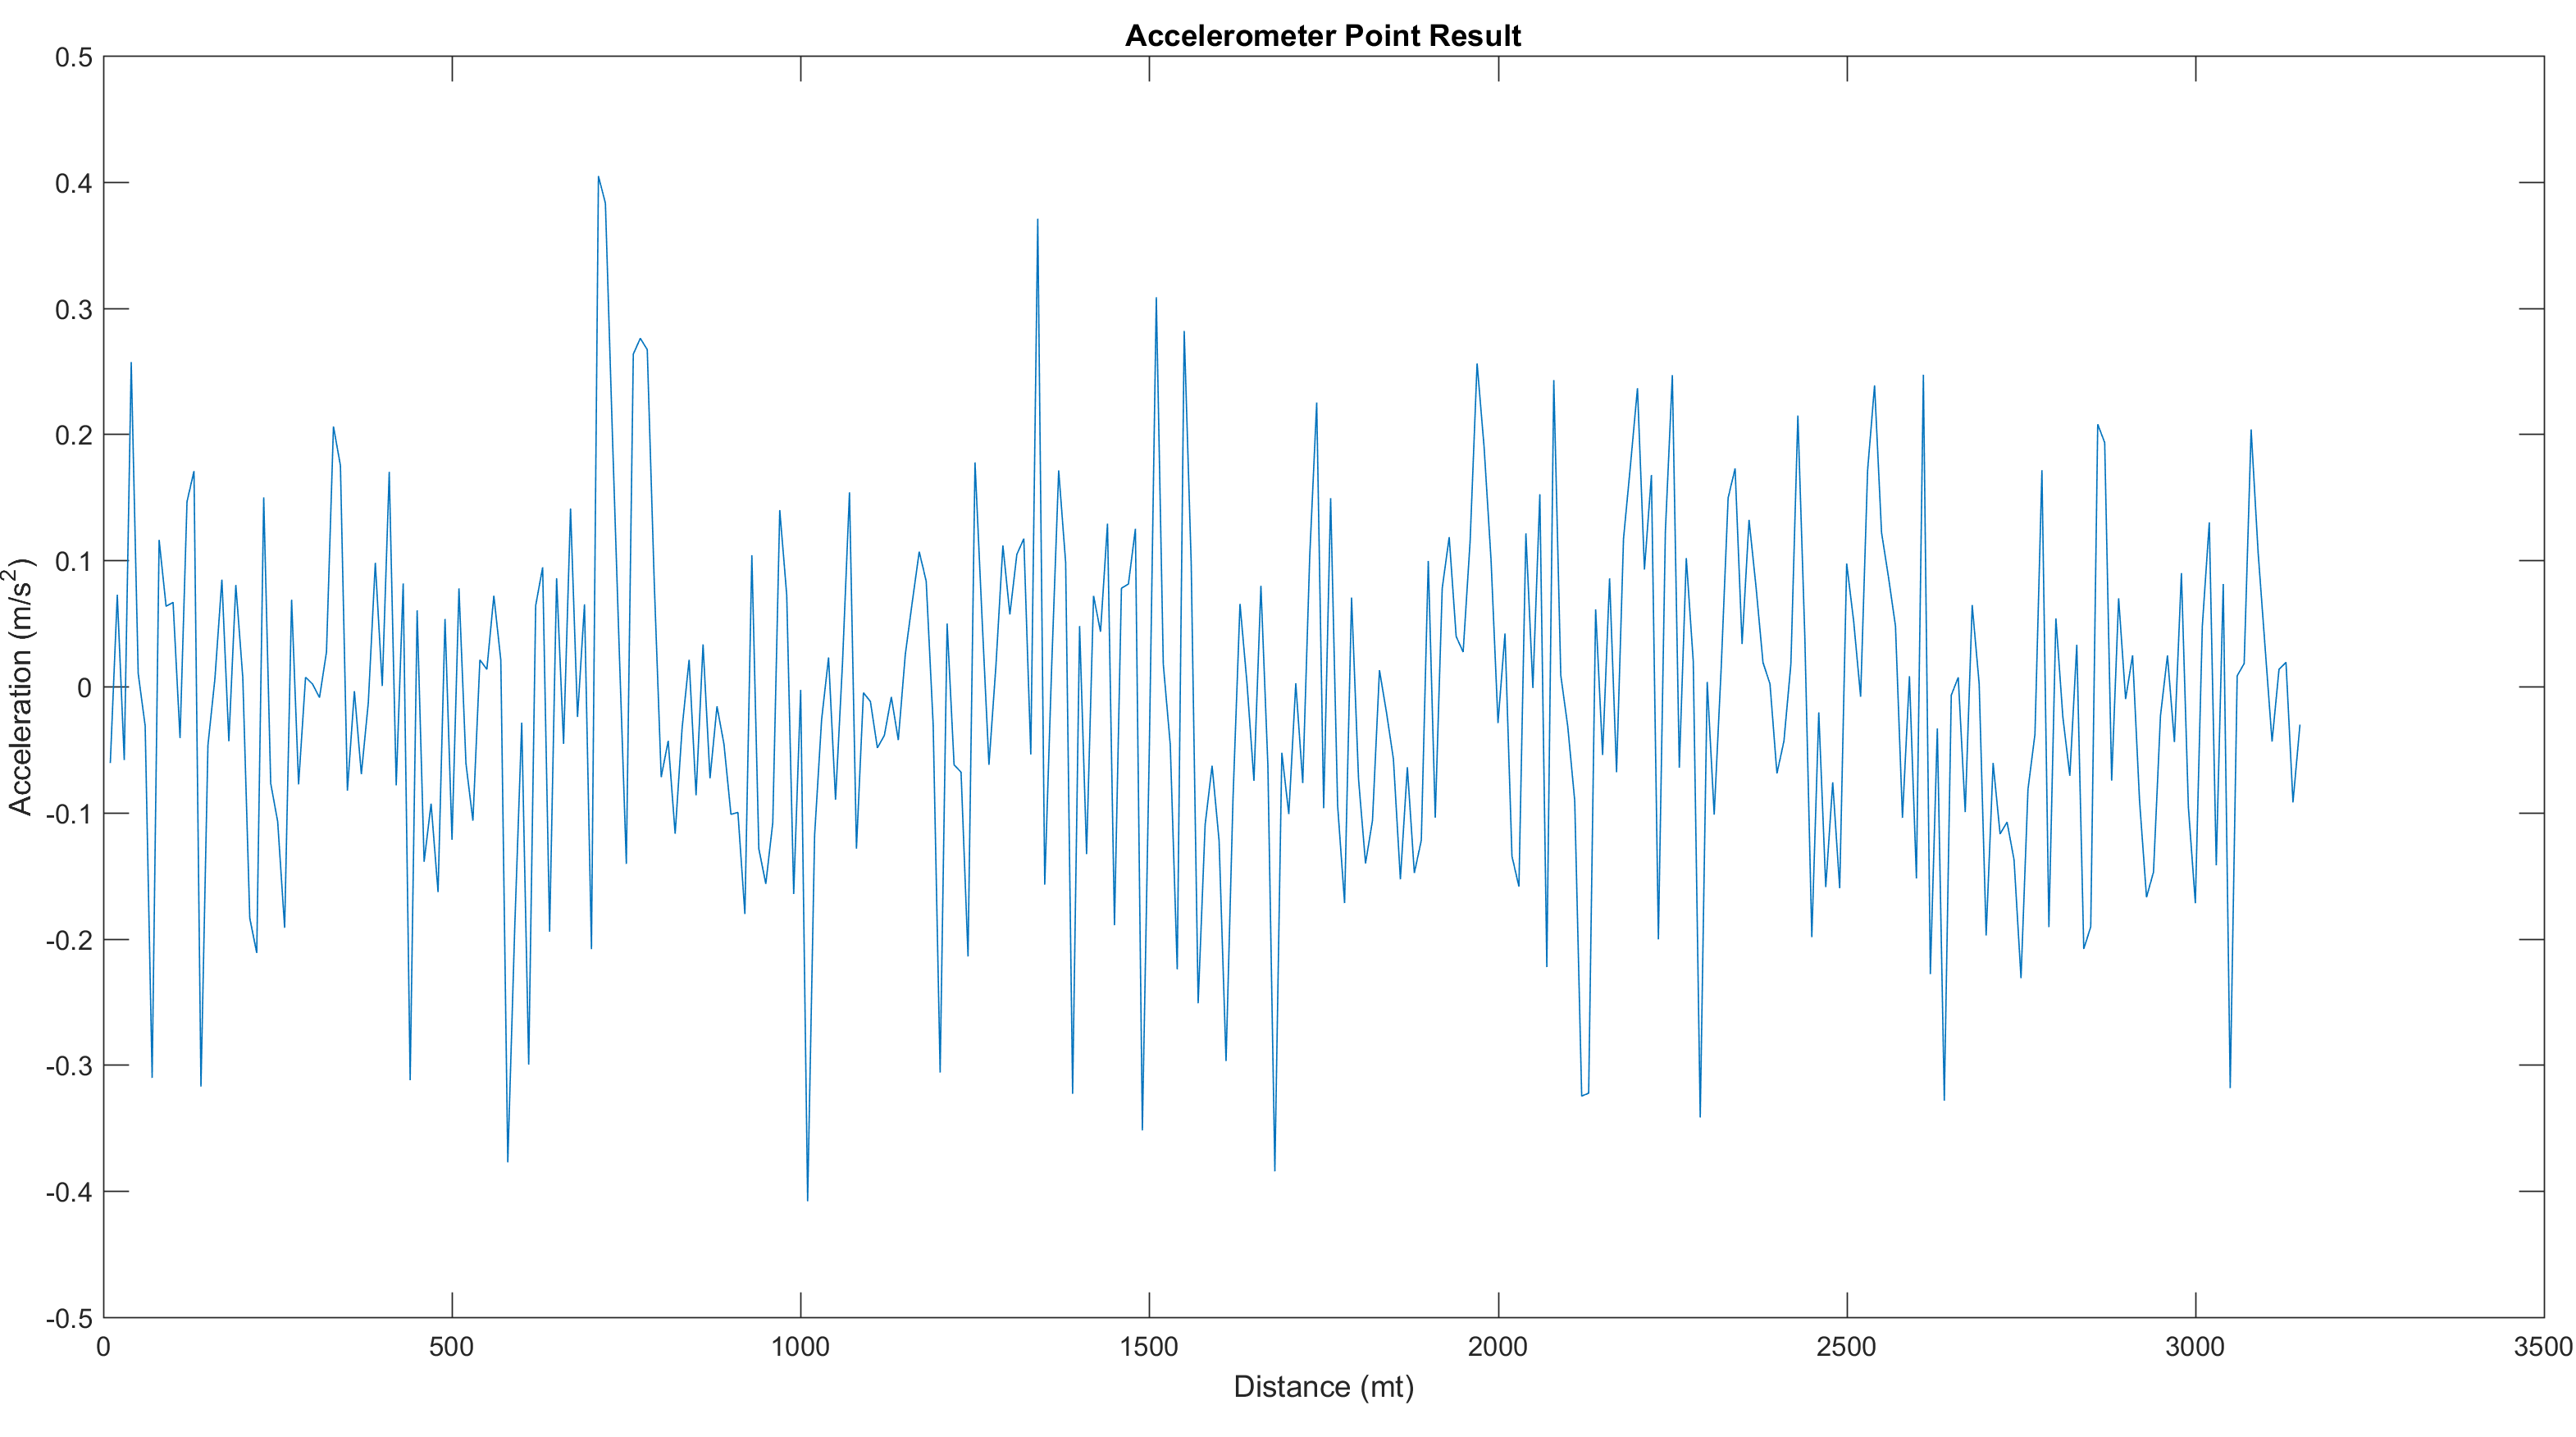
\includegraphics[scale=0.14]{SPAFinal}
\caption{Final Result}
\end{figure}\label{fig:Simple Accelerations Points Final Result}
\end{description}


\subsection{Critical Points}\label{ssc:Critical Points}
This index is very useful as it allows us to locate the most damaged points on the road surface.
Allowing us to identify holes, bumps, and all those types of anomalies that passing over one of they could damage the vehicle and cause an inadequate feeling level of comfort at the driver \ref{ch:Introduction}.
For this, be informed of the localisation of these anomalies,  allows the driver during navigation, to avoid them or reduce speed in their proximity.
This index is processed and calculated only by the vertical acceleration signal because the presence of high peaks corresponds to high-energy events generated by the road-vehicle vibration and can, therefore, be associated with "anomalies" on the surface.
Each of these points will be properly geolocated on the Earth's surface, as for the other indexes, also in this case, at each acceleration signal, GPS coordinates will be associated.	

Following the processing of the signal, which will be properly smoothed, in order to identify the critical points, the final value will be calculated as follows:

\begin{center}
${\large \kappa_{i} \thinspace = 0 \qquad	if \quad	threshold_{min} \thinspace <= \thinspace a_{i} \thinspace <= \thinspace threshold_{max}}$\\

${\large \thinspace \kappa_{i} \thinspace = a_{i} \qquad if \quad a_{i} \thinspace > \thinspace threshold_{max} \quad or \quad a_{i} \thinspace < \thinspace threshold_{min}}$
\end{center}

where:
\begin{itemize}
\item $\kappa_{i}$ is the index results.
\item $a_{i}$ is the acceleration signal.
\end{itemize} 
Following several inspections and controls on the signal, it was possible to identify two thresholds $\left(threshold_{min},\quad threshold_{max}\right)$.
If the signal falls within this range then it does not correspond to an anomaly, vice-versa if it is outside it, represent an anomaly.

Considering the following signal:

\begin{figure}[H]
\centering
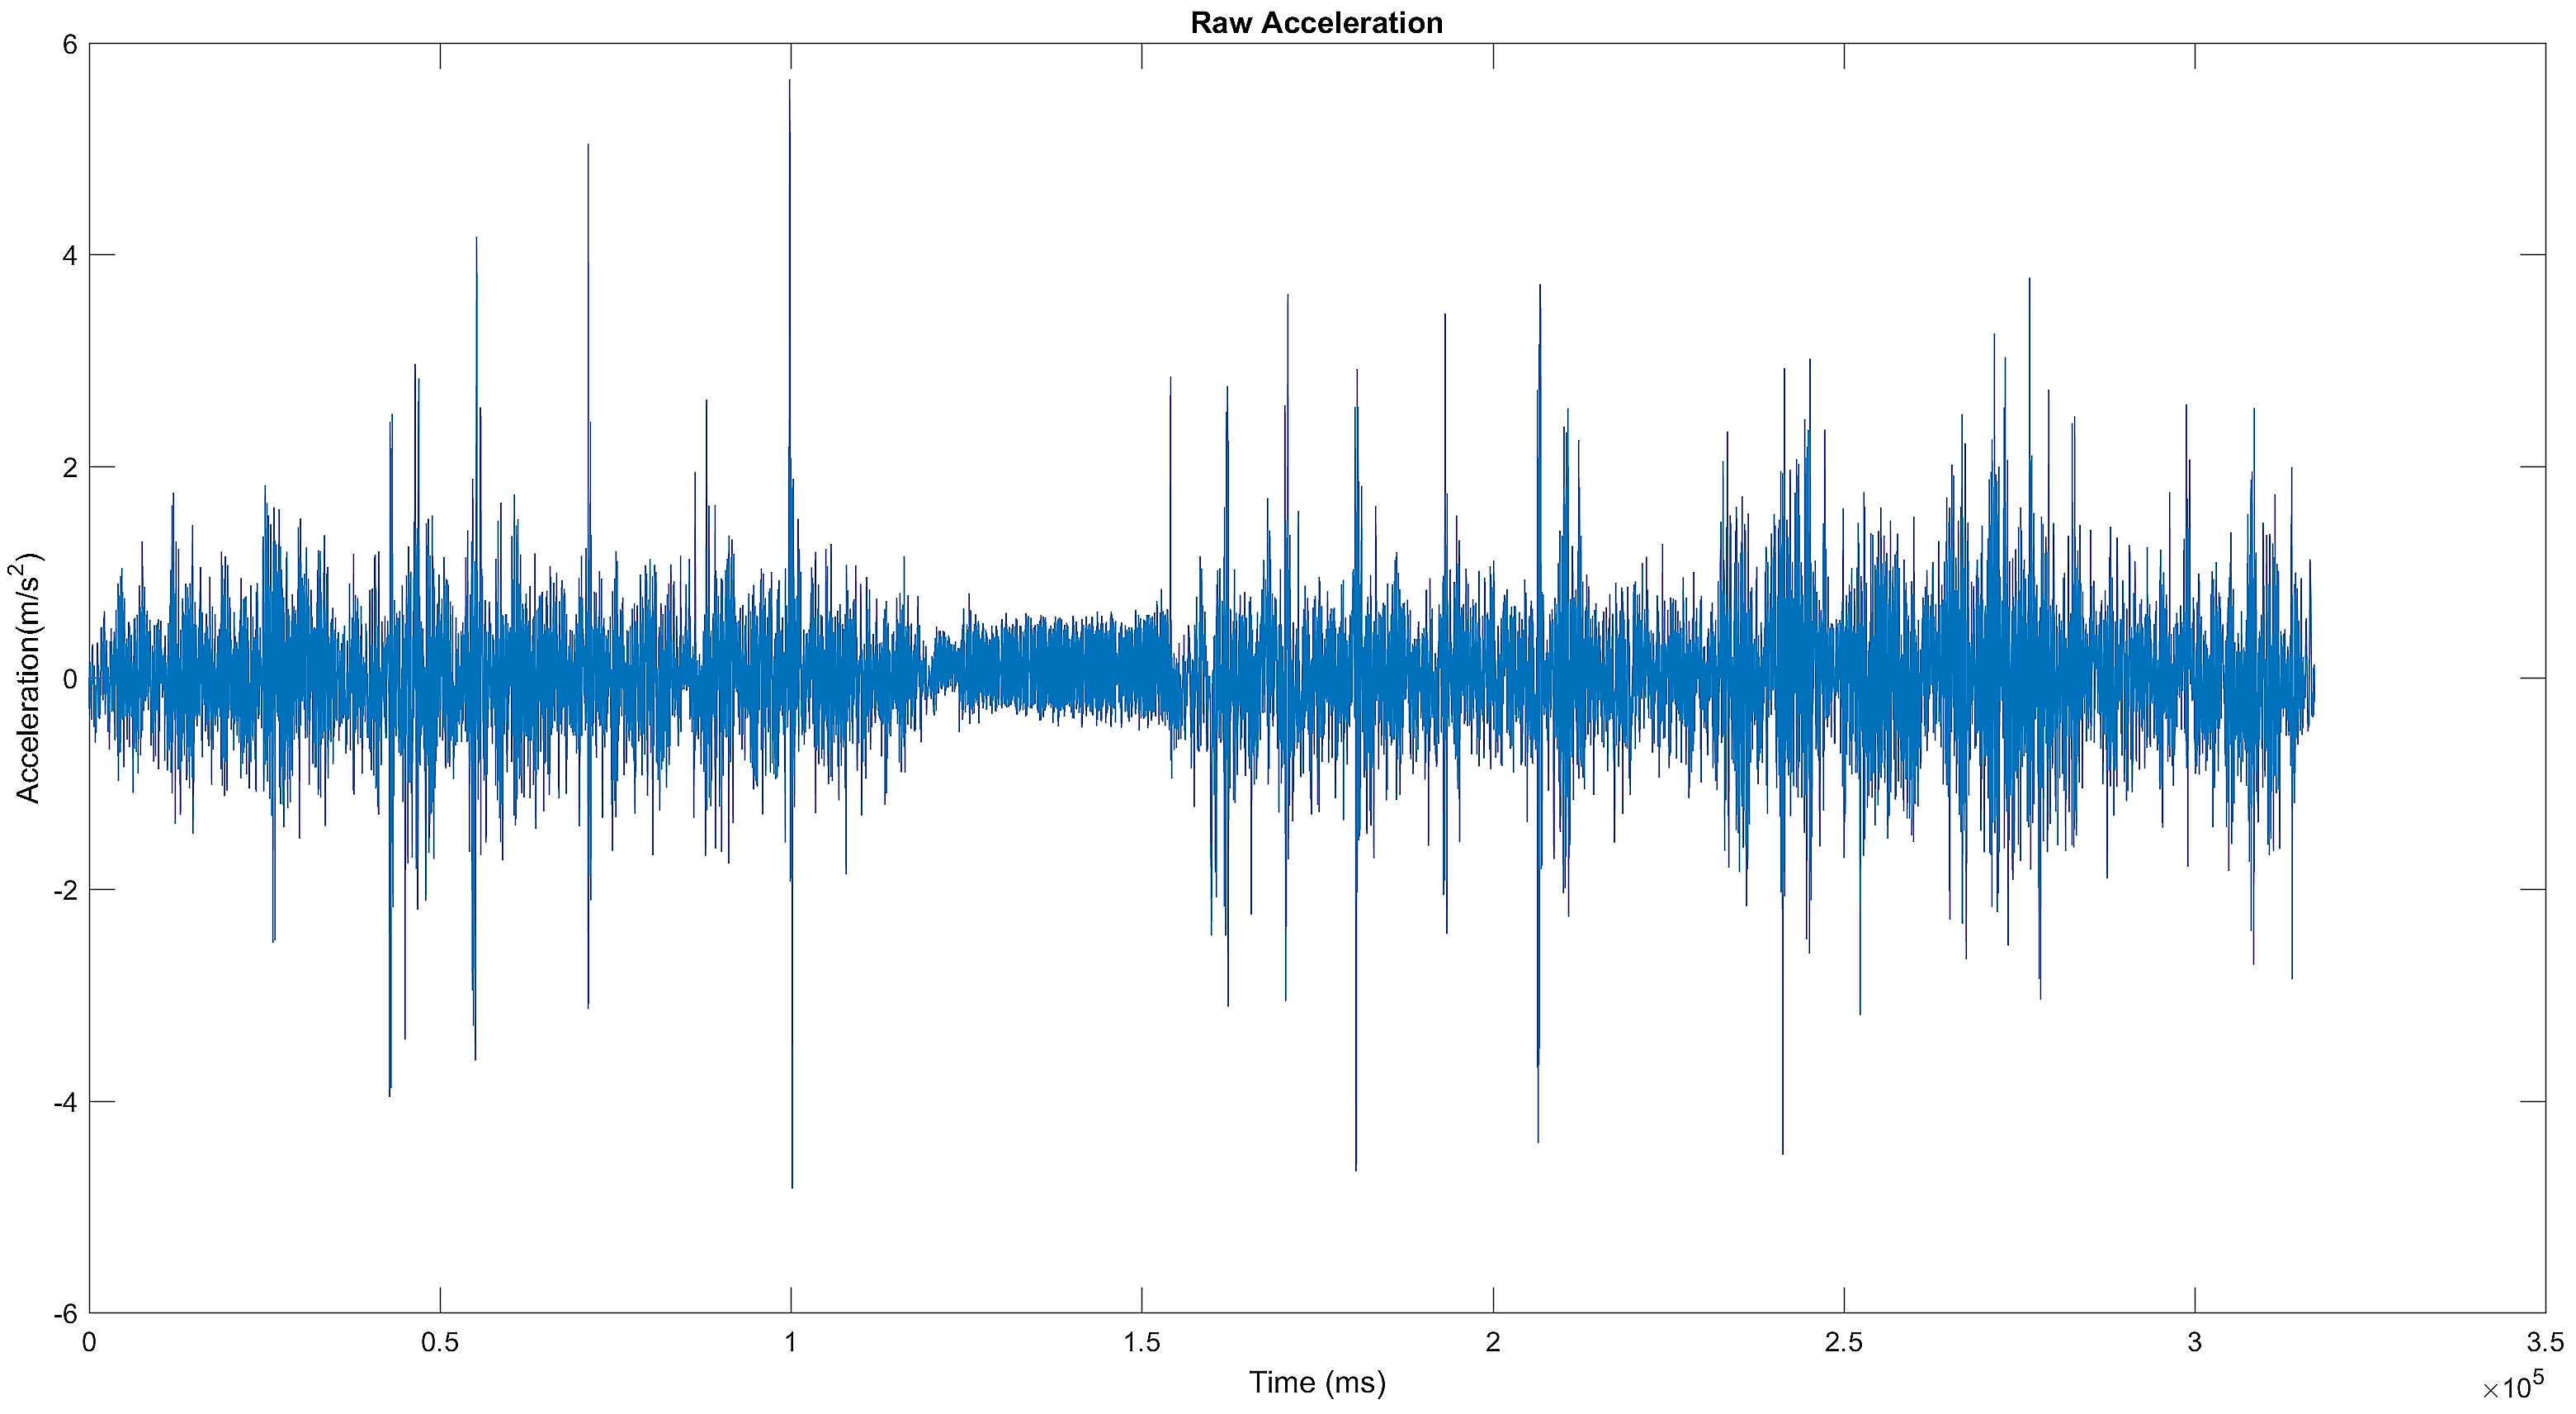
\includegraphics[scale=0.16]{CPRaw}
\caption{Original Signal}
\end{figure}

The steps for its calculation are:

\begin{description}
\item[1. Accelerometer Reorientation:] First of all it is applied the procedure of Accelerometer reorientation explained in Chapter\ref{ch:Data Analysis} (section:\ref{sc:Accelerometer Reorientation}, on page: \pageref{sc:Accelerometer Reorientation}).
\item[2. GPS points division:] Next, the GPS points are subdivided according to the methodology explained in Chapter\ref{ch:Data Analysis} (section:\ref{sc:GPS points division}, on page: \pageref{sc:GPS points division}).
\item[3. Filtering Engine Vibrations:] This filter is the first operation that is performed on the data, in which the noise components generated by the engine will be smoothed, according to the application seen in the Chapter\ref{ch:Data Analysis} (section:\ref{sc:Data Filtering}, on a page:\pageref{sssc:Remove Engine Vibrations Filter}).
The result of the application of the filter on the signal shown above is:
 \begin{figure}[H]
\centering
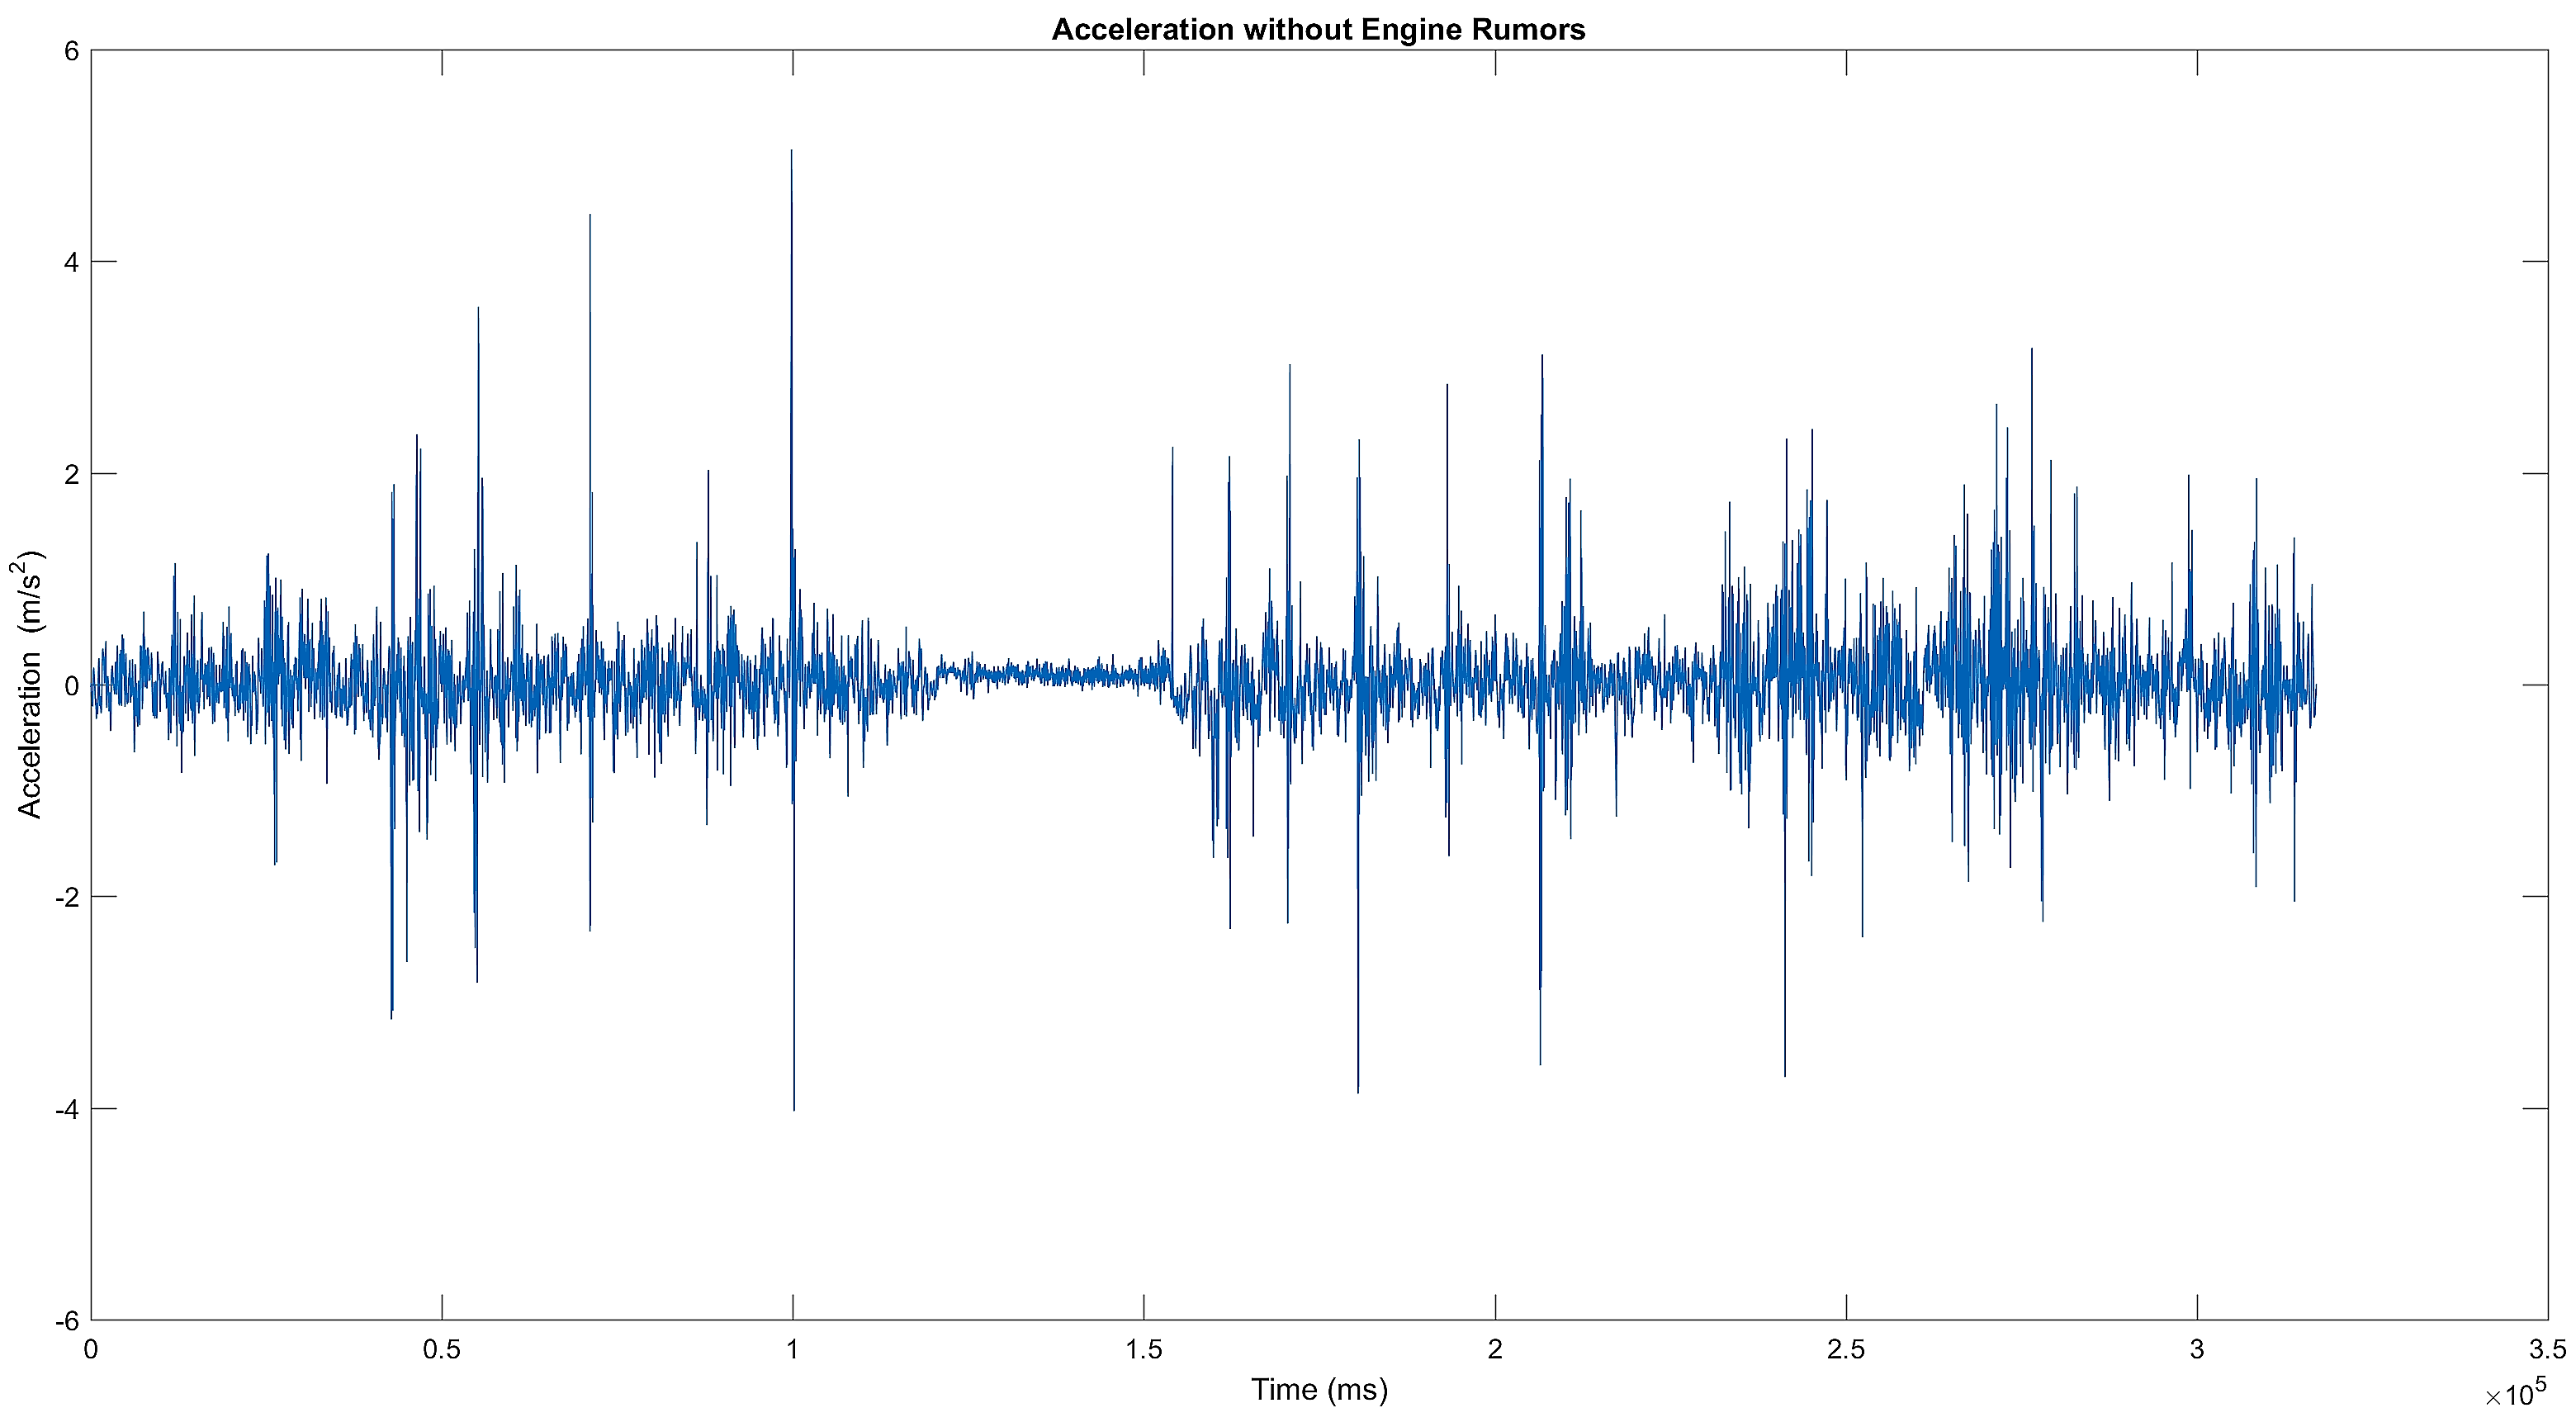
\includegraphics[scale=0.14]{CPNoEngine}
\caption{Signal Without Engine Vibrations}
\end{figure}
\item[4. Zero Velocity Filter:] After applying the first filter, this is also applied, as it is explained in the Chapter\ref{ch:Data Analysis} (section:\ref{sc:Data Filtering}, on page:\pageref{sssc:Zero Velocity Filter}).
The result of the application of the filter on the signal shown above is:
 \begin{figure}[H]
\centering
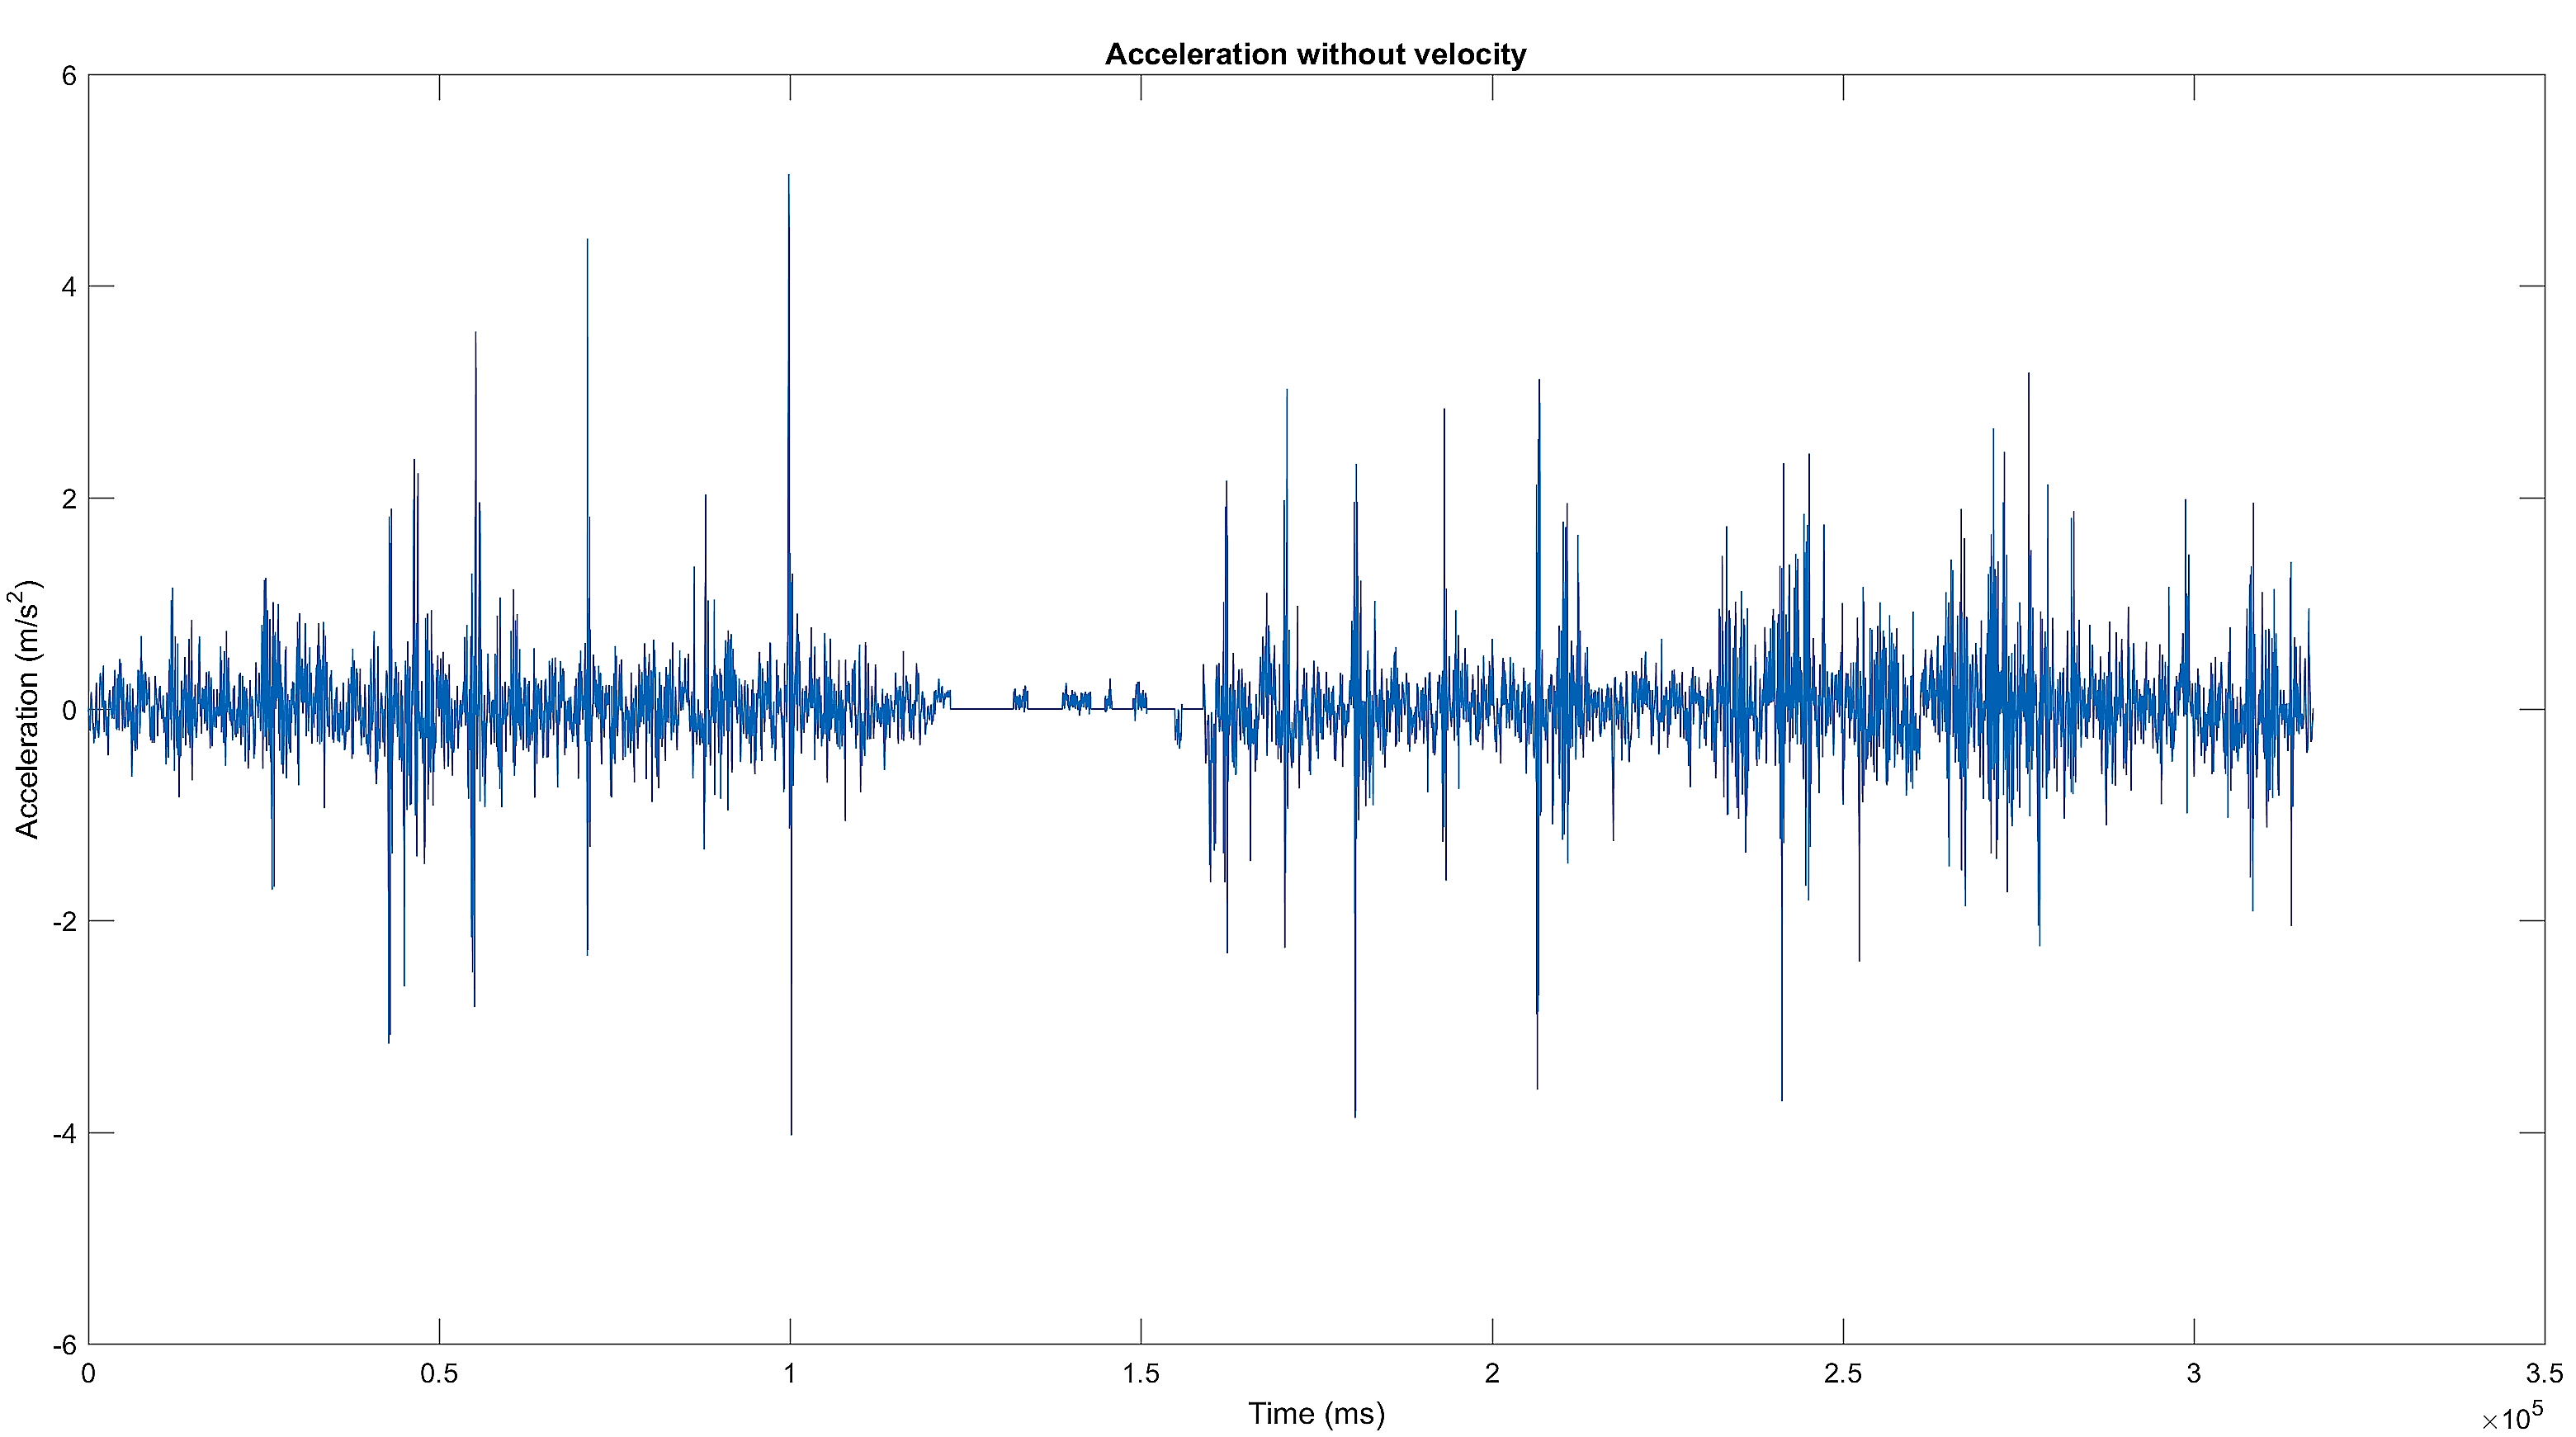
\includegraphics[scale=0.14]{CPNoVelocity}
\caption{Null Velocity Removed}
\end{figure}
\item[5. Determining Critical Points:] In this step, the critical points are identified, according to the formula explained above. The result is shown in the figure.
The result of the application of this filter on the signal shown above	 is:
 \begin{figure}[H]
\centering
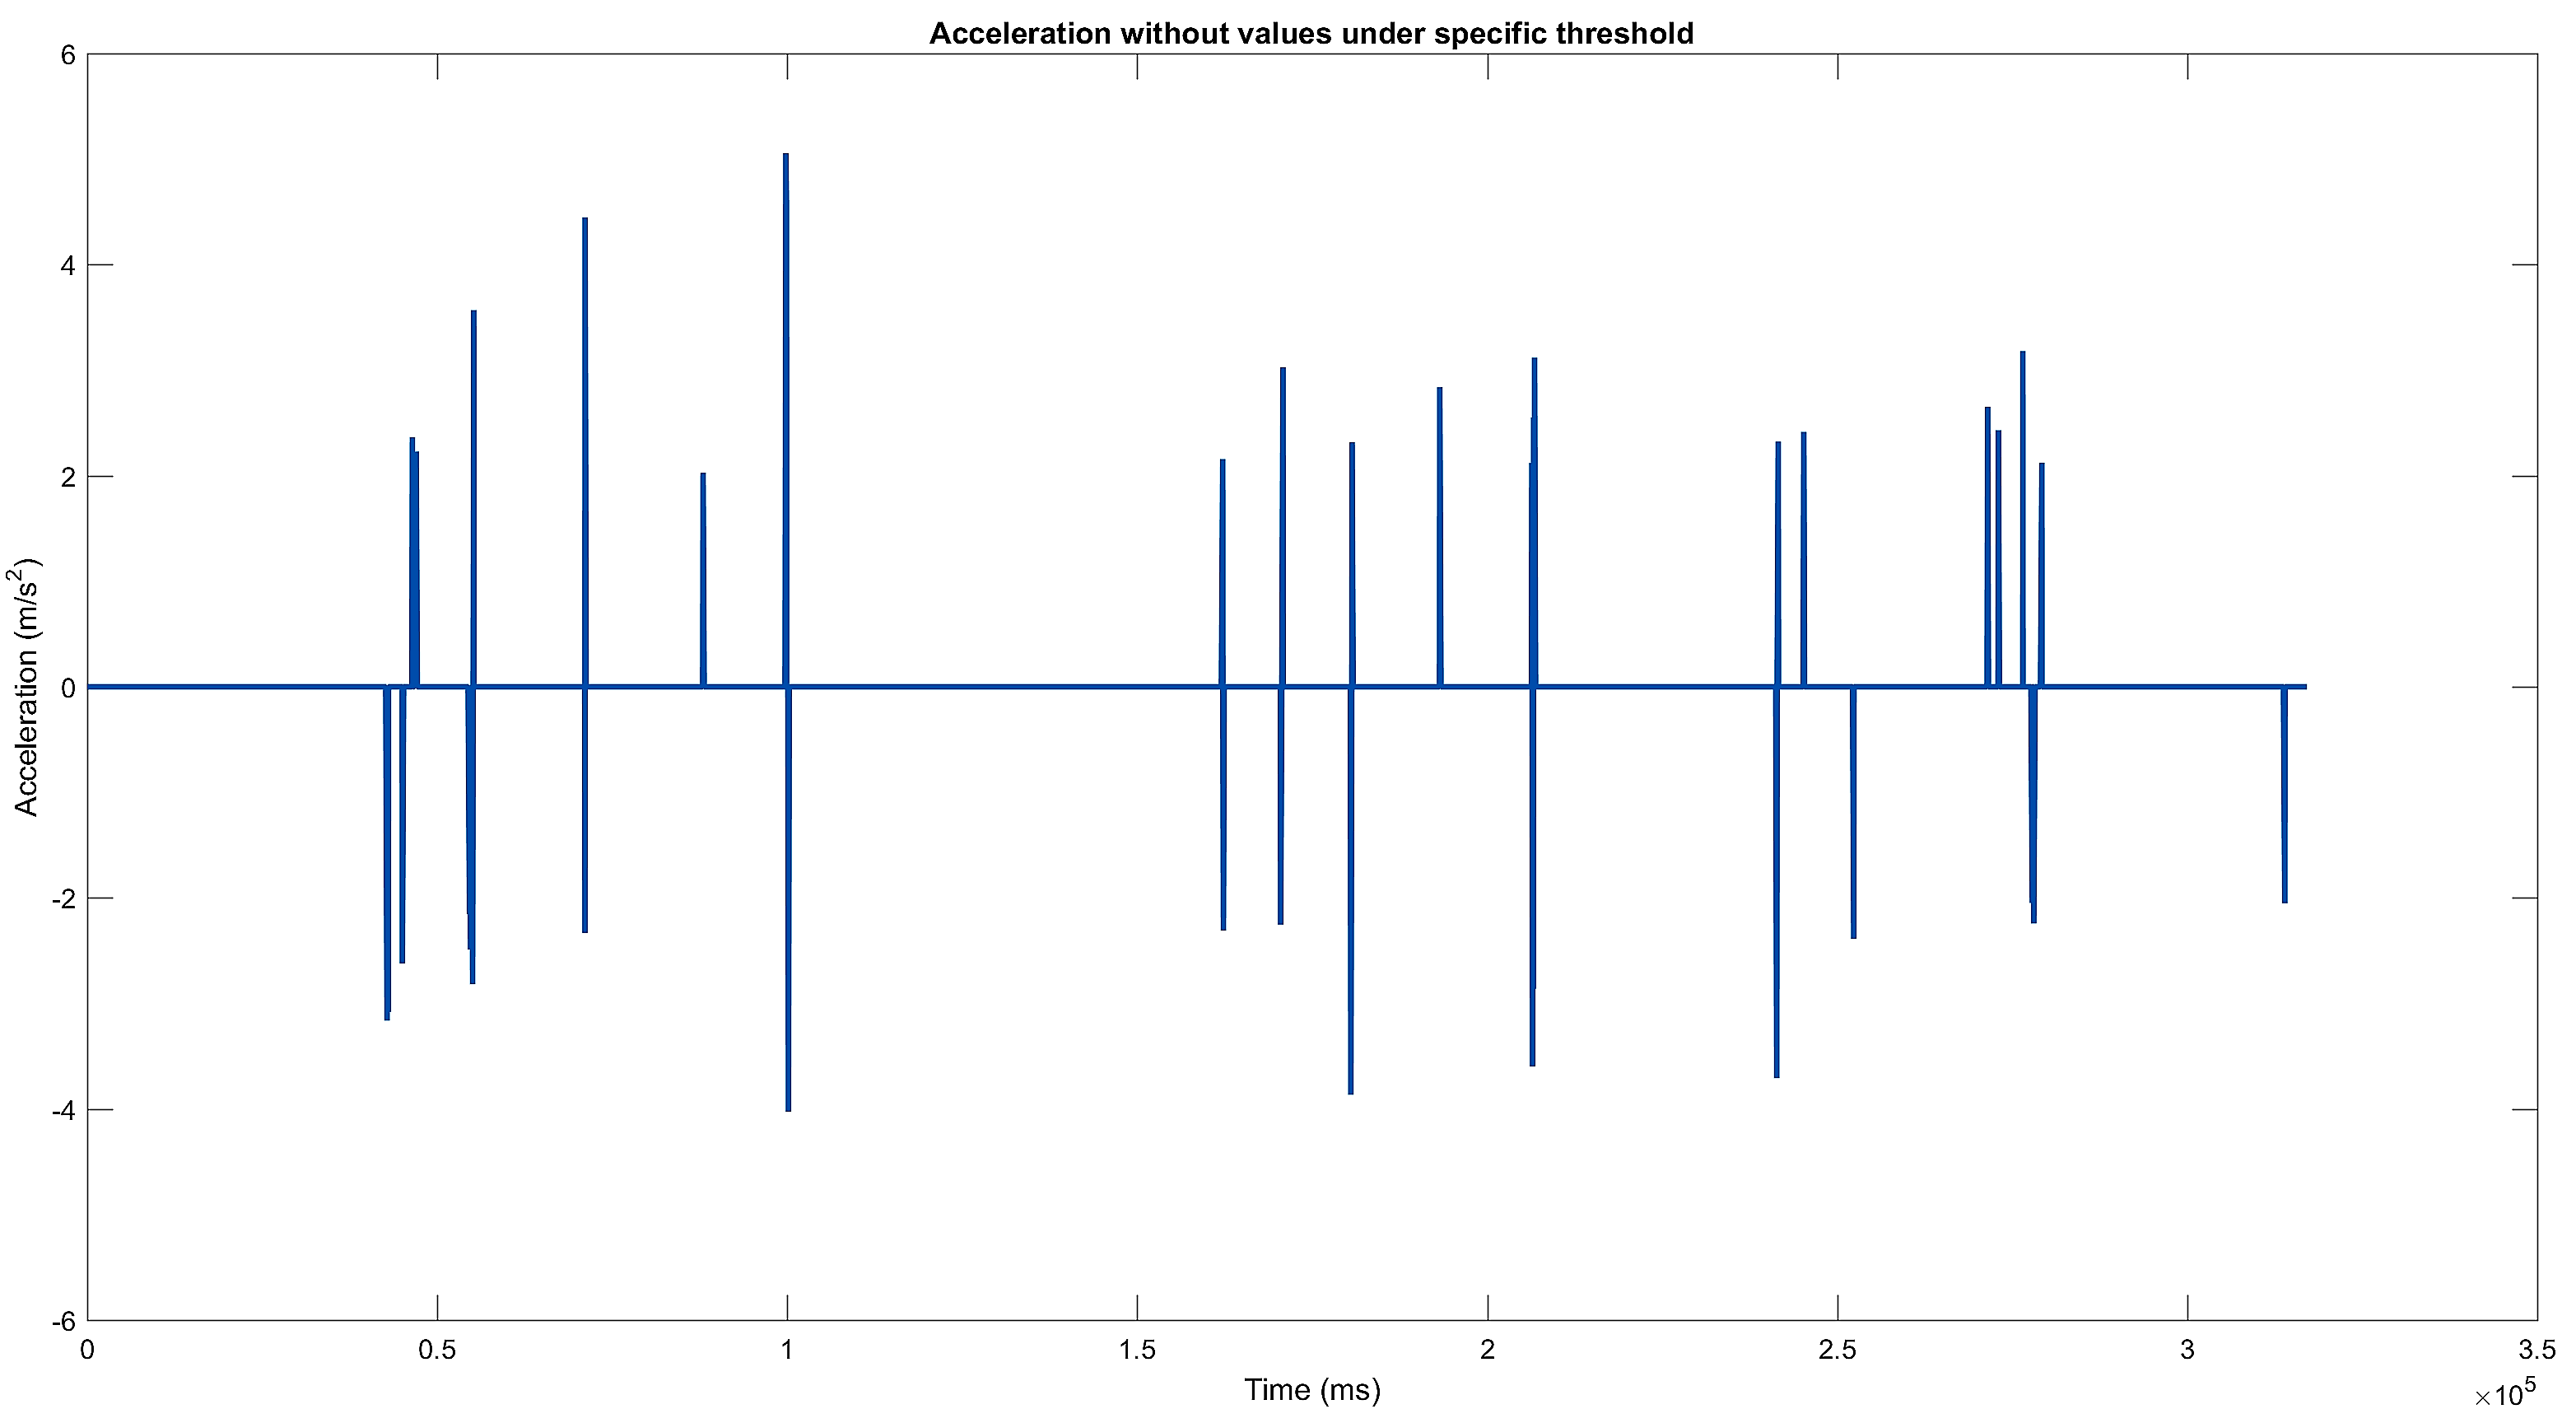
\includegraphics[scale=0.16]{CPUnderTH}
\caption{Results Final}
\end{figure}\label{fig:Critical Points Final Result}
\item[6. Grouping the points too close each other:]  Defined the critical points, there is a final step to be carried out. Following the GPS points division(\ref{sc:GPS points division}), it may happen in the previous step, that consecutive points are selected, or in any case too close each other, which refers to the same anomaly (in fact, the signal is similar for a given small time due the high recording frequency, so the same anomaly would have more associated signals). It is necessary to incorporate these signals into a single point, for this purpose, the Haversine formula(\ref{ssc:Haversine Formula}) was used. 
When a set of points is identified, they will be grouped within a certain distance ($ds$) and enclosed within a single GPS point. Similarly to the final $\kappa$ value, it will be identified as the average of the points belonging to this set, because they refer to the same anomaly and will have similar values.
\end{description}




\clearpage
\subsection{IRI}\label{ssc:IRI}
As we have seen in Chapter\ref{ch:IRI} (on page, \pageref{ch:IRI}), where this index is widely explained and how it is calculated.
Briefly, represents the most used road roughness index to evaluate and manage road infrastructure. IRI is defined as the ratio between the sum of vehicle-wheel displacements of a standard vehicle.
It will be determined following several steps:

\begin{itemize}
\item Double integration of acceleration.
\item Calculation of IRI from obtained displacement data.
\item Correlation phase.
\end{itemize}


\subsubsection{Double Integration Process}
The first step to obtaining an index estimate concerns the dual integration of the vertical acceleration signal, useful in achieving vertical displacement. This process as we have seen in Chapter\ref{ch:Inertial Measurement Unit} may be complex, because the data captured may suffer from various errors (Section \ref{sc:Error}, on page \pageref{sc:Error}) that are accumulating during the travel.
In order to obtain an approximate realistic result, it is necessary to perform several data filtering operations (Section\ref{sc:Data Filtering} on page \pageref{sc:Data Filtering}) in order to remove both, noise components and the drift.

Taking the following signal as an example:


\begin{figure}[H]
\centering
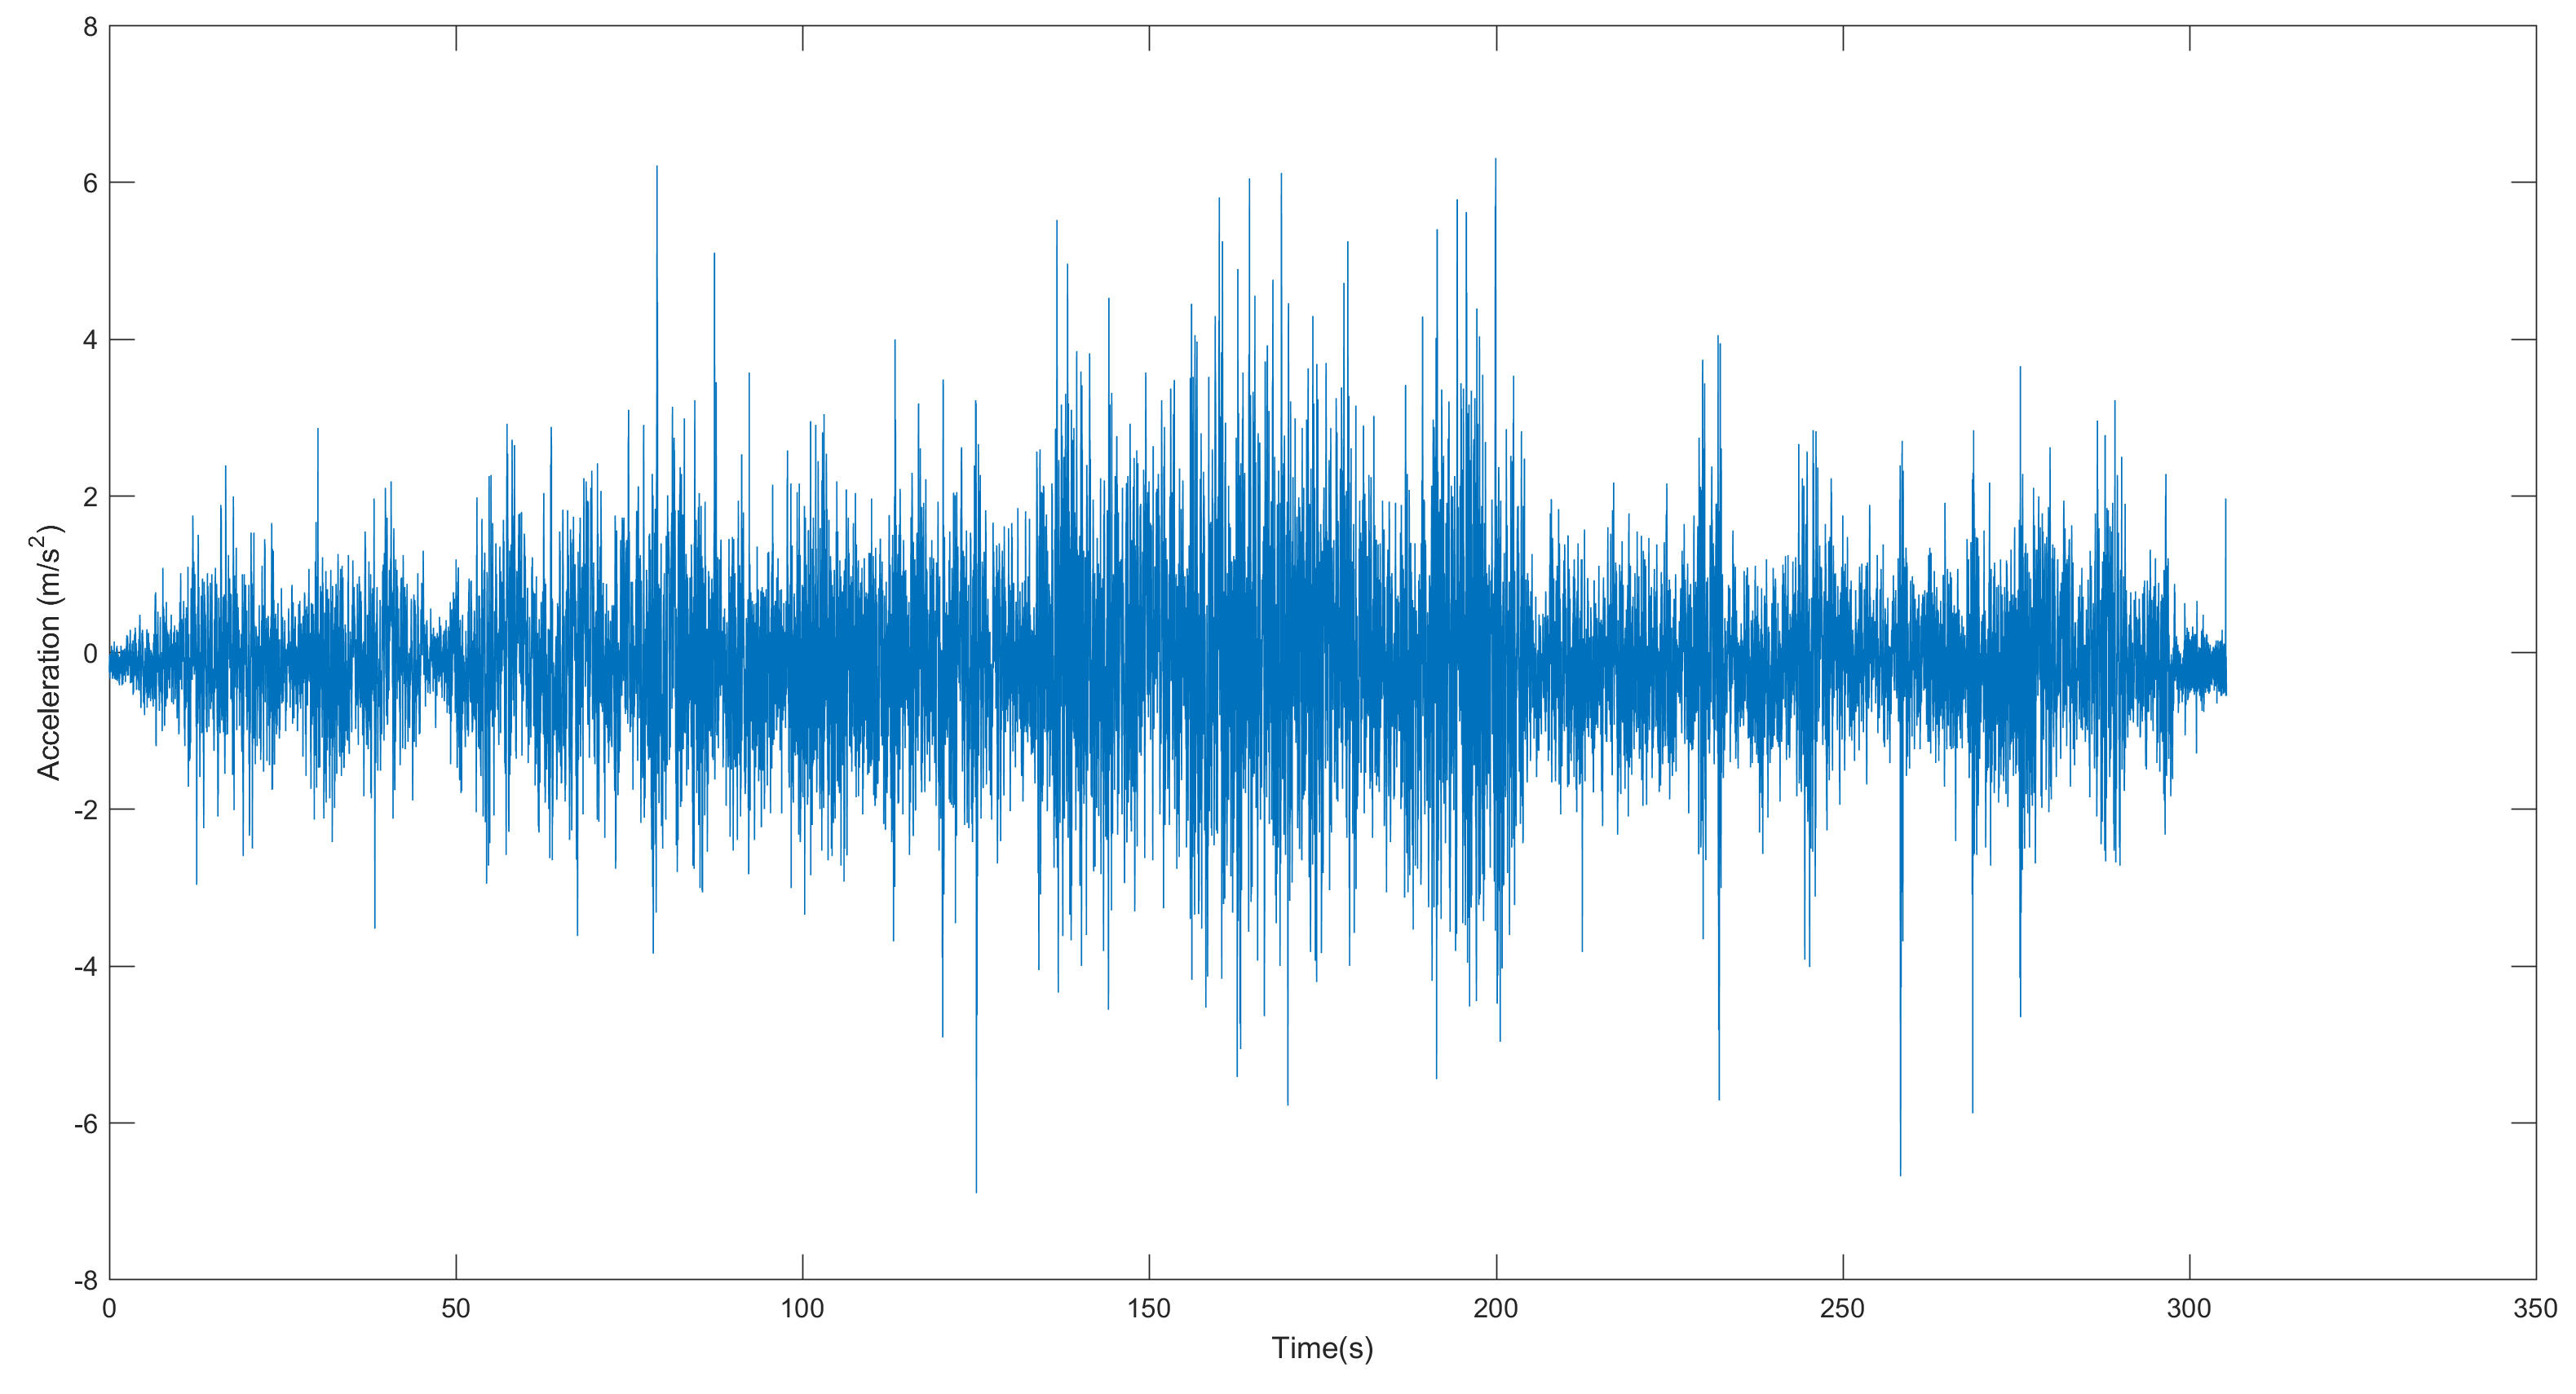
\includegraphics[scale=0.17]{IRIRawSignal}
\caption{Raw Acceleration Signal}
\end{figure}
The double integration process will be carried out as follows:



\begin{description}
\item[1. Accelerometer Reorientation:] First of all, it is applied the procedure of Accelerometer reorientation explained in Chapter\ref{ch:Data Analysis} (section:\ref{sc:Accelerometer Reorientation}, on page: \pageref{sc:Accelerometer Reorientation}).
\item[2. GPS points division:] Next, the GPS points are subdivided according to the methodology explained in Chapter\ref{ch:Data Analysis} (section:\ref{sc:GPS points division}, on page: \pageref{sc:GPS points division}).
\item[3. Filtering Engine Vibrations:] This filter is the first operation that is performed on the data, in which the noise components generated by the engine will be smoothed, according to the application seen in the Chapter\ref{ch:Data Analysis} (section:\ref{sc:Data Filtering}, on page:\pageref{sssc:Remove Engine Vibrations Filter}).
\item[4. Zero Velocity Filter:] After applying the first filter, this is also applied, as it is explained in the Chapter\ref{ch:Data Analysis} (section:\ref{sc:Data Filtering}, on page:\pageref{sssc:Zero Velocity Filter}).
\item[5. Application of a FIR moving average filter:] A FIR moving average filter will be applied to the signal according to the principles and features discussed in Chapter\ref{ch:Data Analysis}, Section\ref{sc:Data Filtering}, on a page:\pageref{p:moving_average}.
This filter starts to smooth the signal.
The result obtained is shown in the figure:
\begin{figure}[H]
\centering
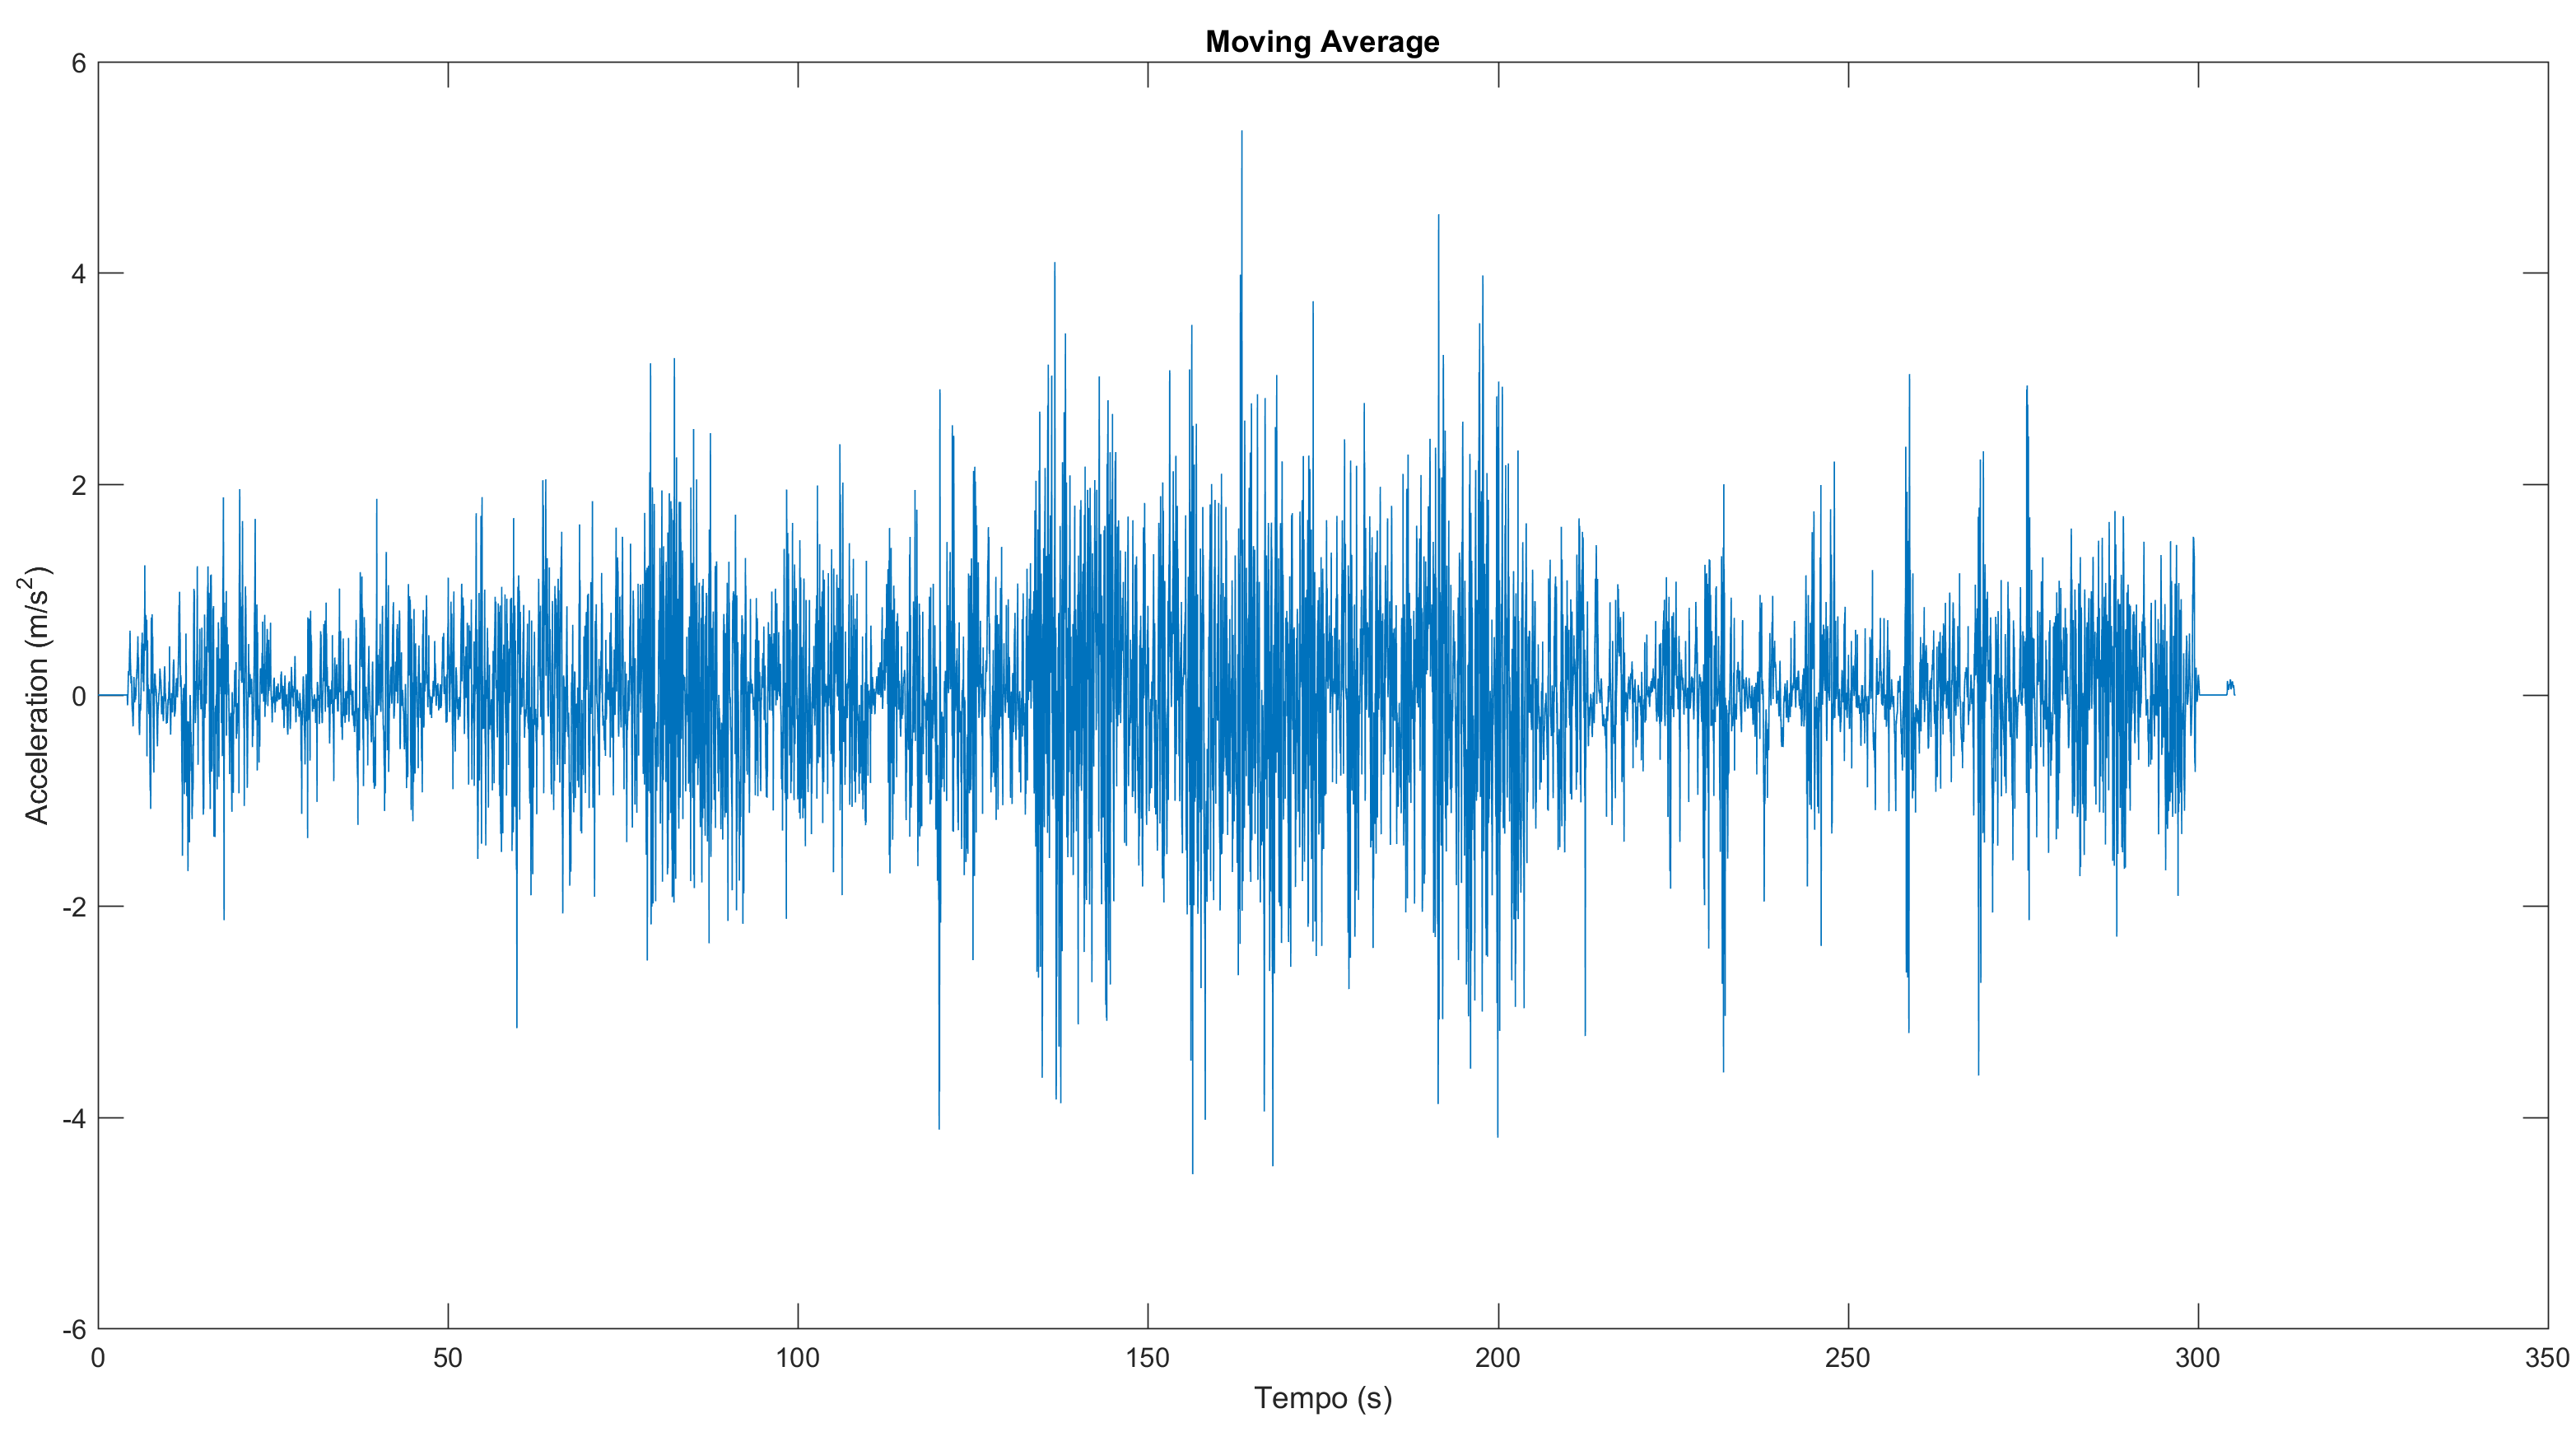
\includegraphics[scale=0.17]{IRIMovingAverage}
\caption{Application of a FIR moving average filter on signal}
\end{figure}
\item[6. Filtering Operations]
In this phase will be performed the filtering of the signal through the application of two filters.
Various Fourier analysis(\ref{sc:Fast Fourier Transform}) were performed on the signals.
It emerged that they had various peaks around the frequency of $0 \thinspace Hz$. These values that fall around this frequency are also called DC Components(\ref{ssc:Digital Filtering}), they cause a high drift(\ref{sc:Error}) during the integration phase leading to incorrect results (as shown in the figure\ref{fig:Integration of Raw Data}).
For this reason, it is necessary to eliminate them from the signal. The idea is to allow the passage of the signal that goes over this frequency (more than $0 \thinspace Hz$), and isolate the DC components, around the frequencies of $0 \thinspace Hz$. To do this and for its principles, a High Pass Filter was used, according to the features explained in Chapter\ref{ch:Data Analysis}, in section(\ref{ssc:High Pass Filter}), on a page: \pageref{ssc:High Pass Filter}.
Following its application, a Low-Pass Filter will also be used, according to the characteristics described in Chapter\ref{ch:Data Analysis}, in section \ref{ssc:High Pass Filter}, on a page:\pageref{ssc:Low Pass Filter}, to smooth the signal without altering his form.
After their applications the result obtained is shown in the figure:
\begin{figure}[H]
\centering
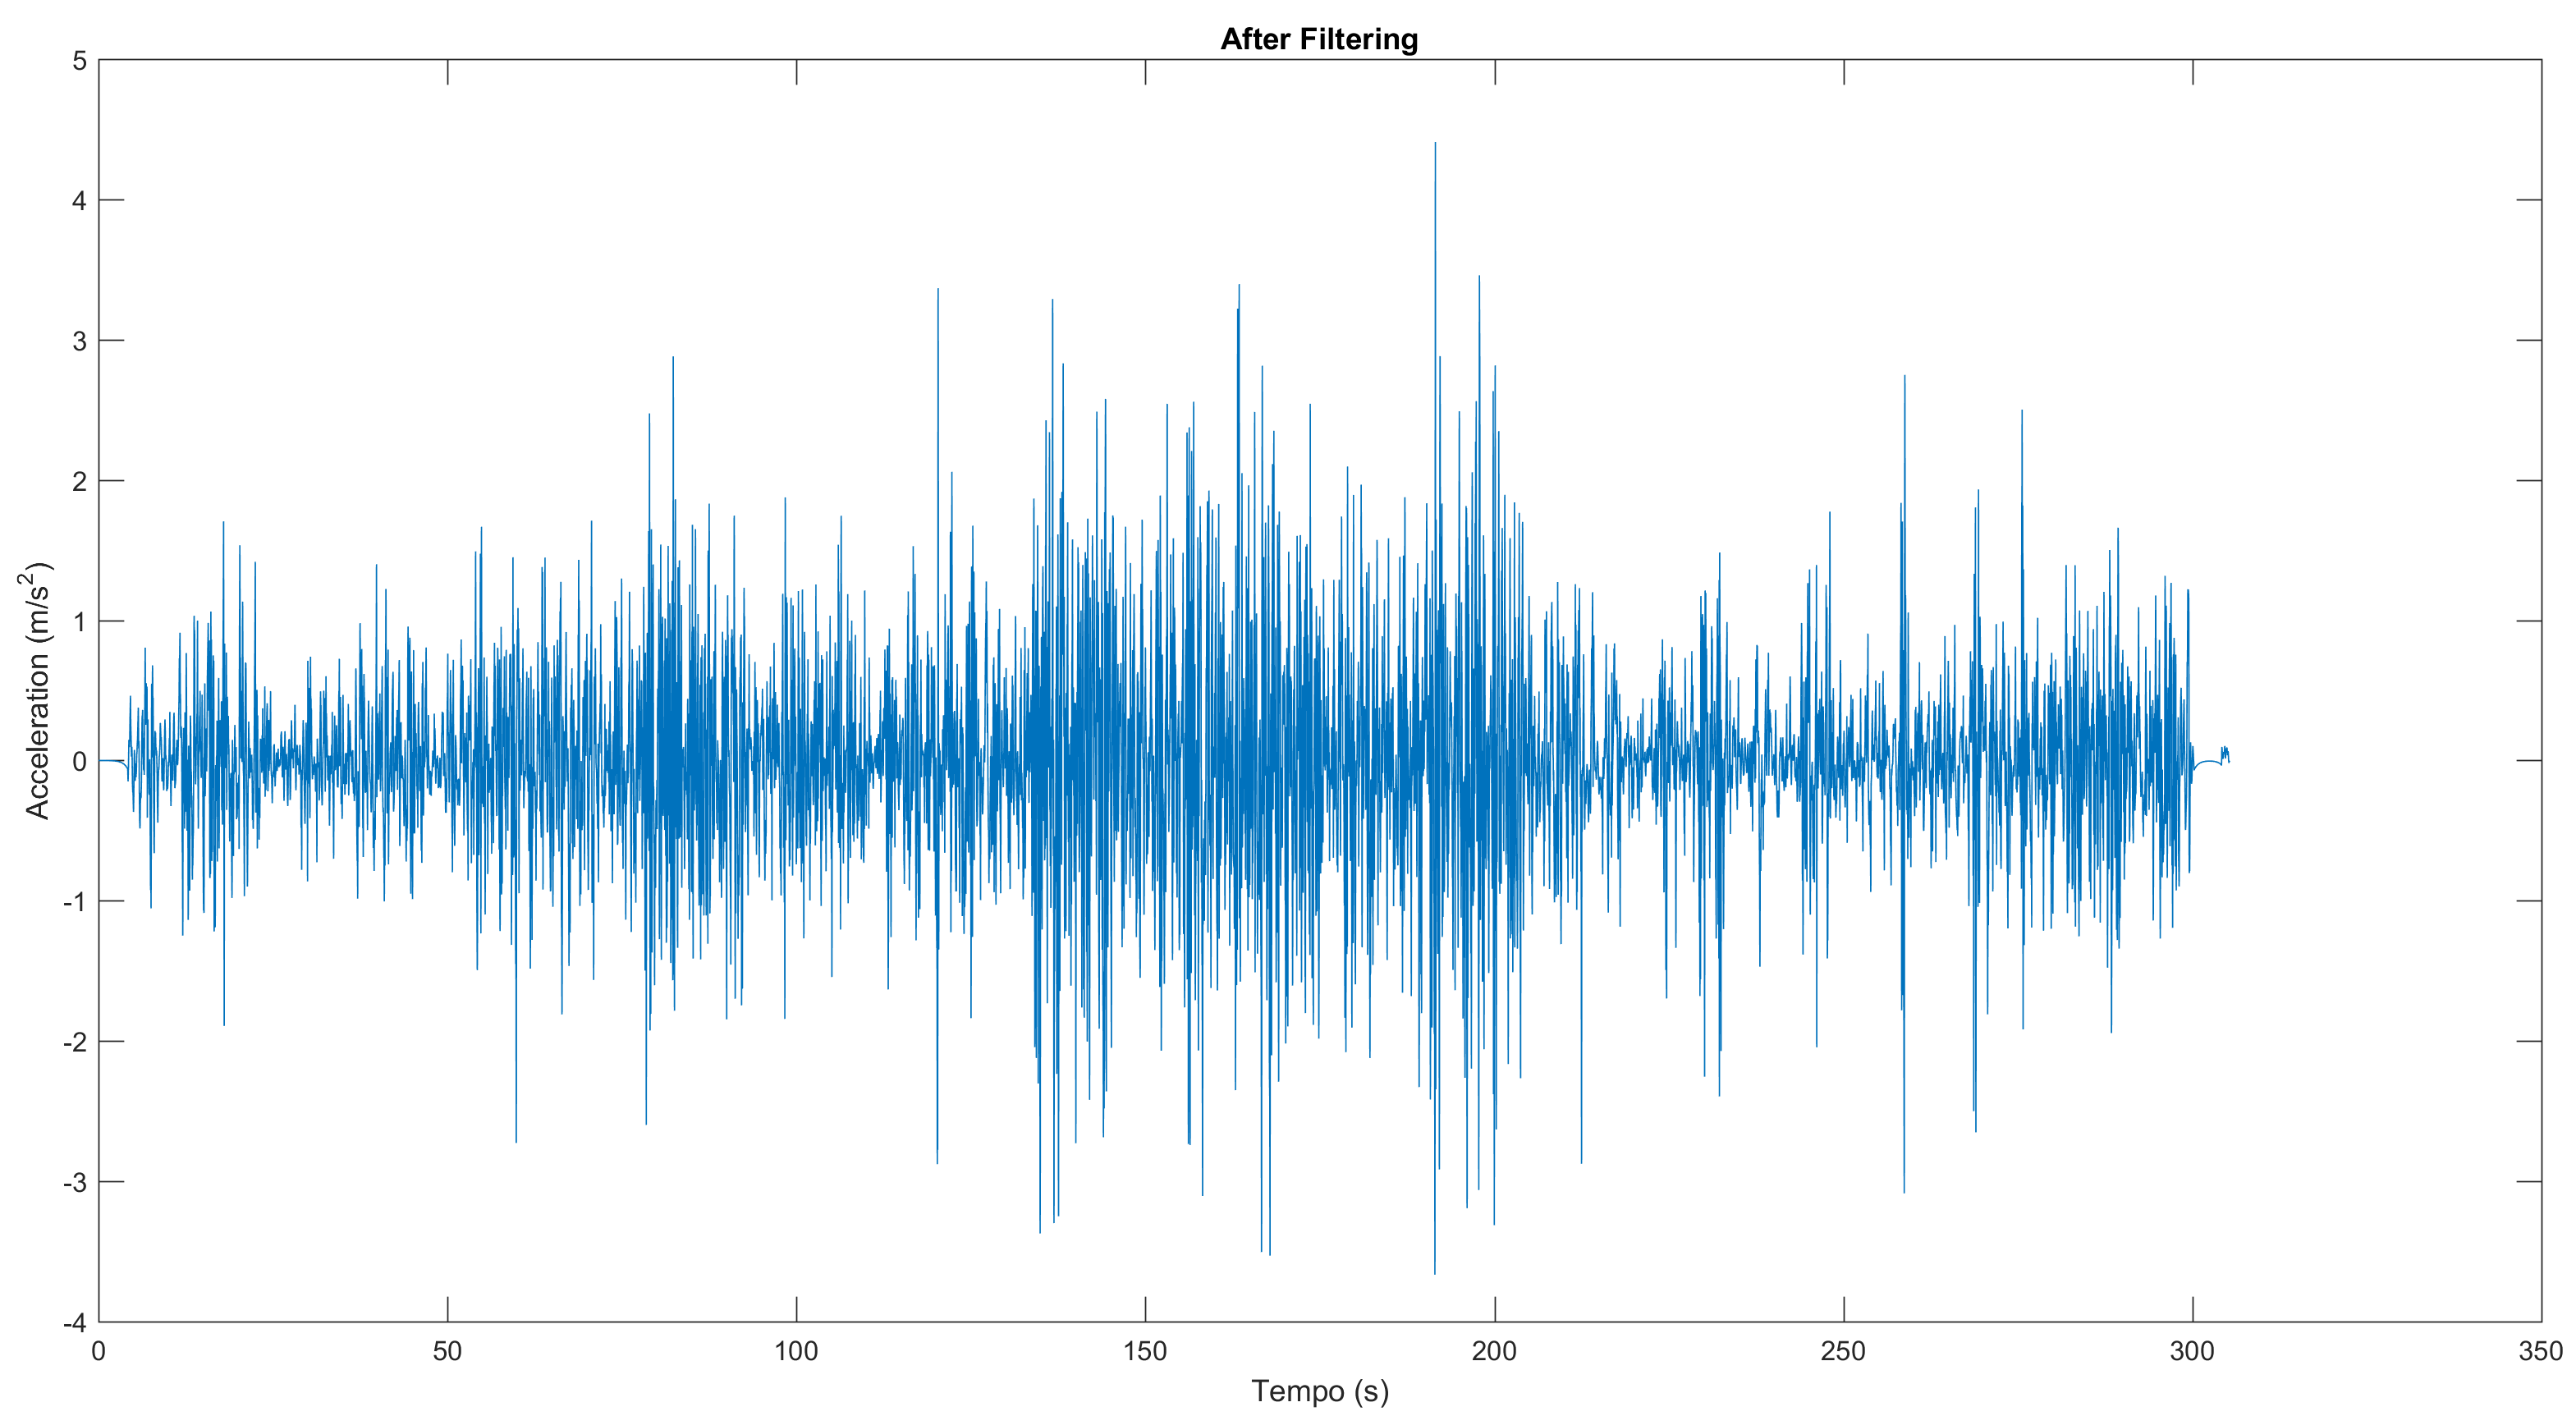
\includegraphics[scale=0.17]{IRIAccelerationFiltering}
\caption{Acceleration Signal after the filters application}
\end{figure}

\begin{figure}[H]
\centering
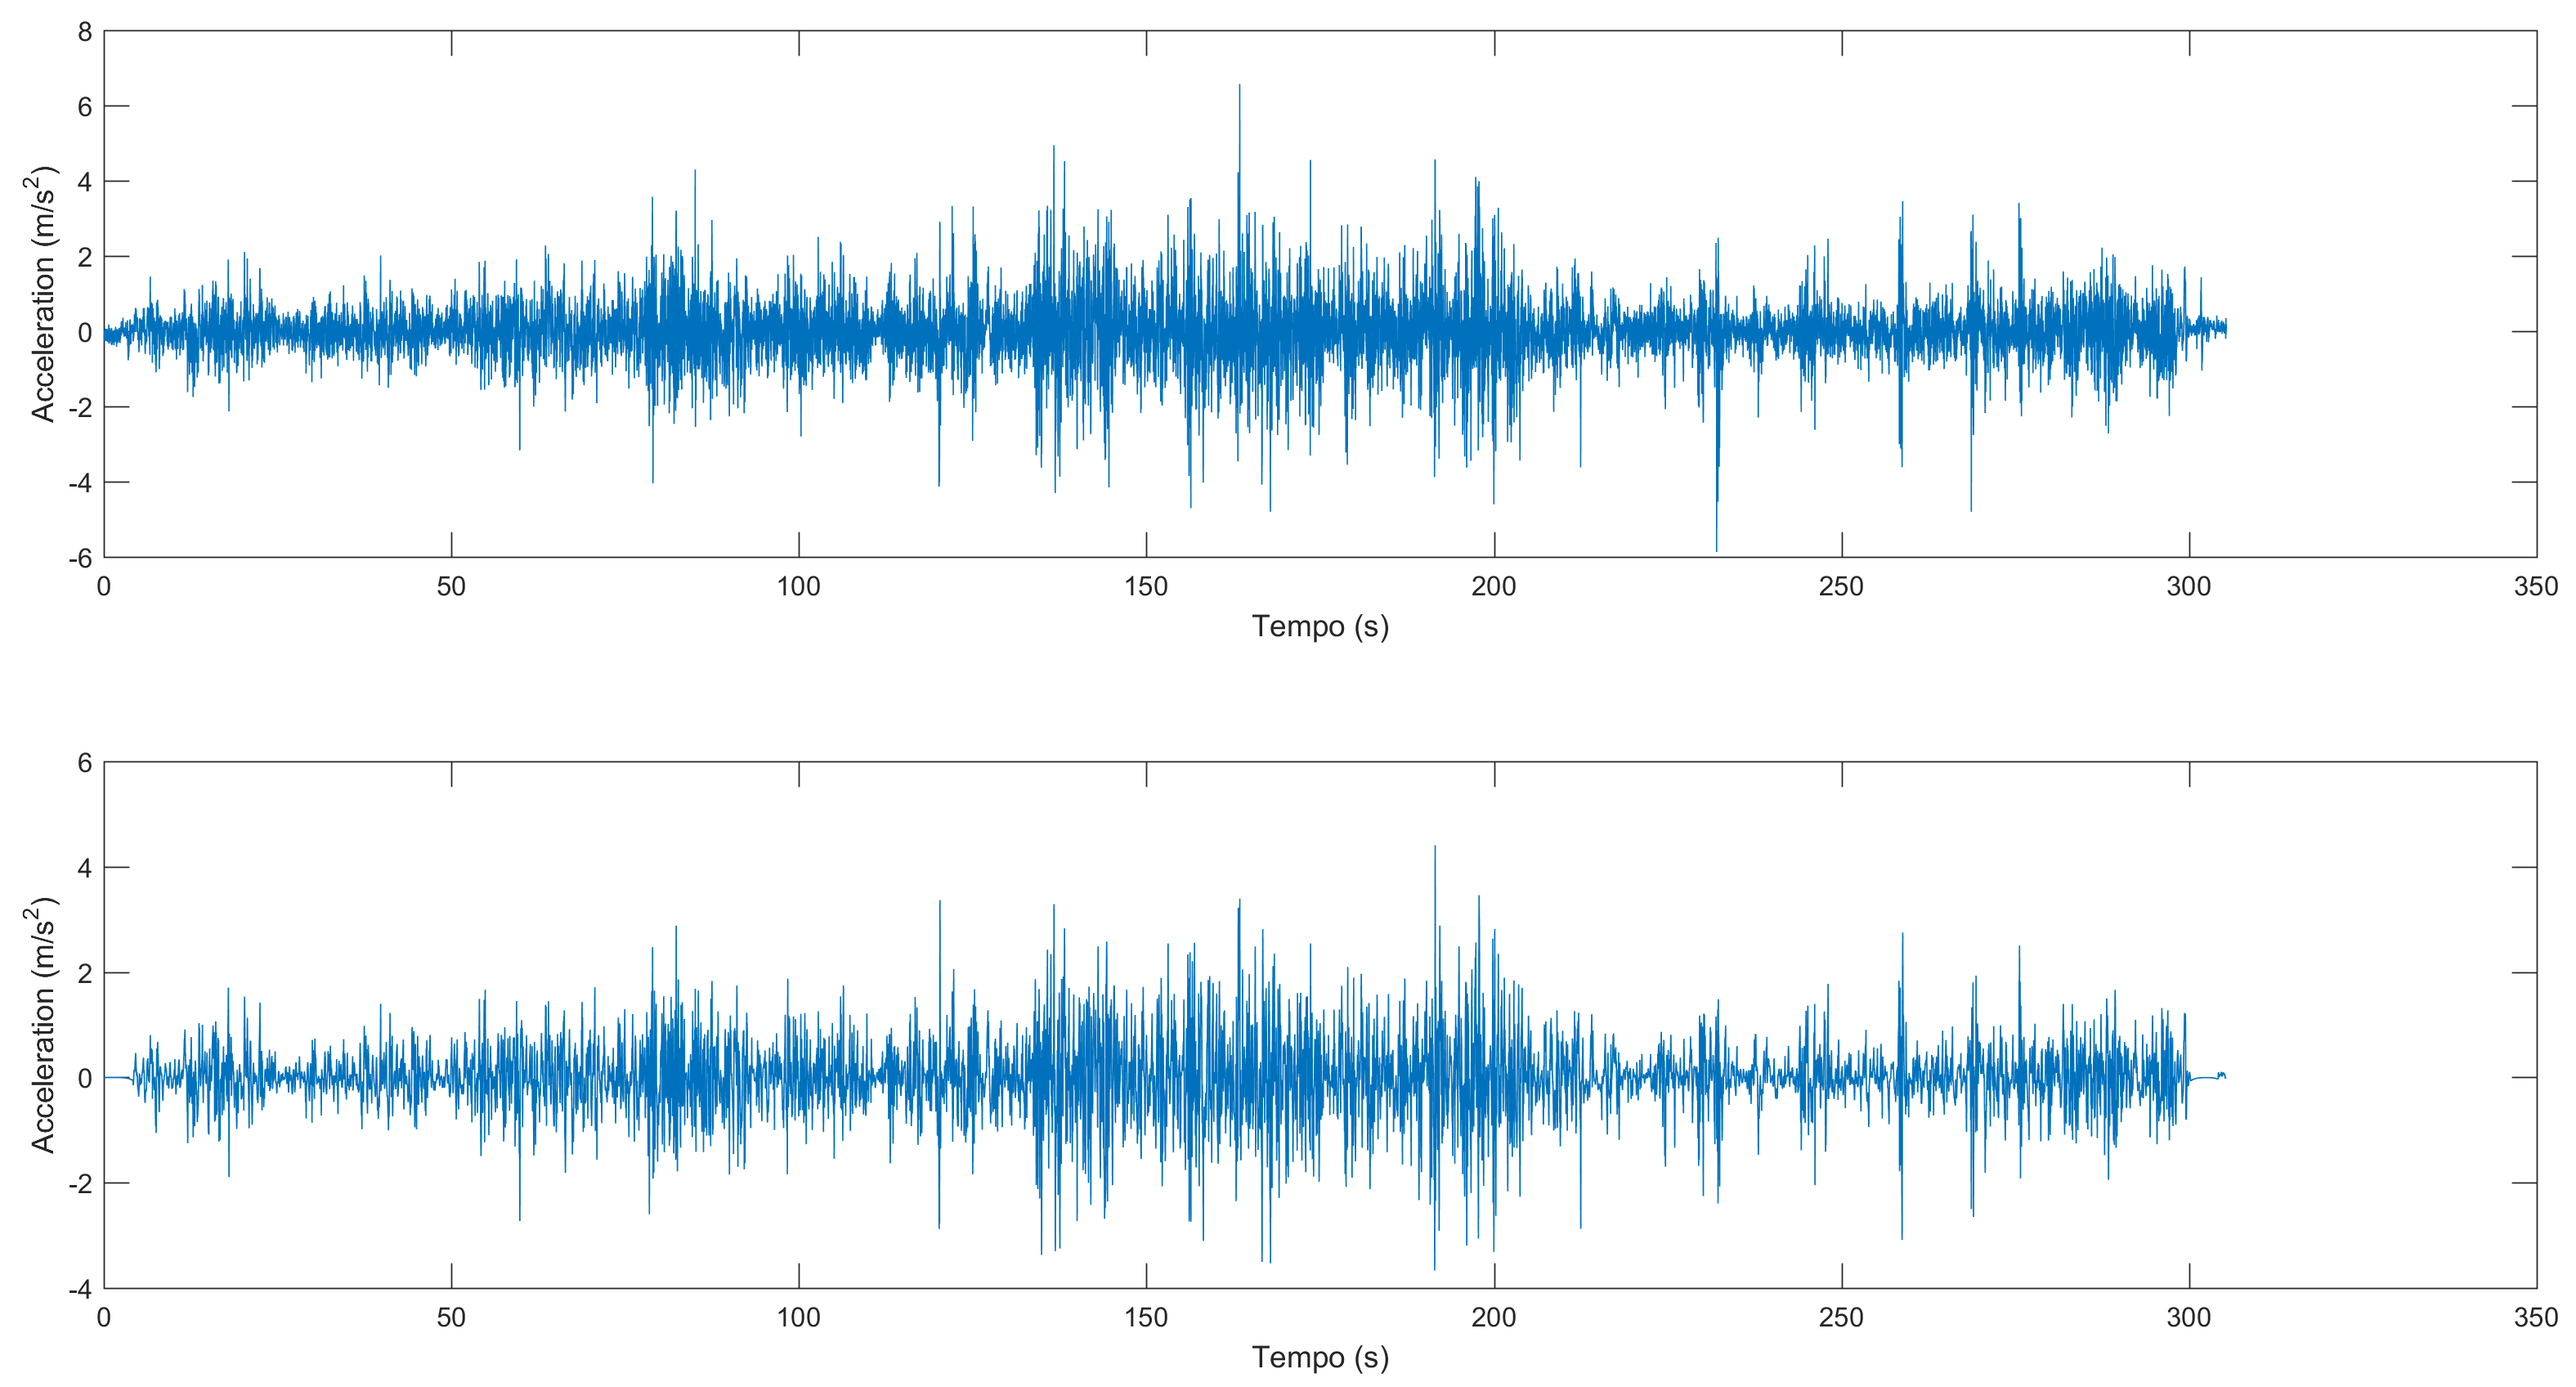
\includegraphics[scale=0.17]{IRITotalFiltering}
\caption{Original Signal compared with the filter Signal}
\end{figure}
\clearpage
While for a more detailed view:
\begin{figure}[H]
\centering
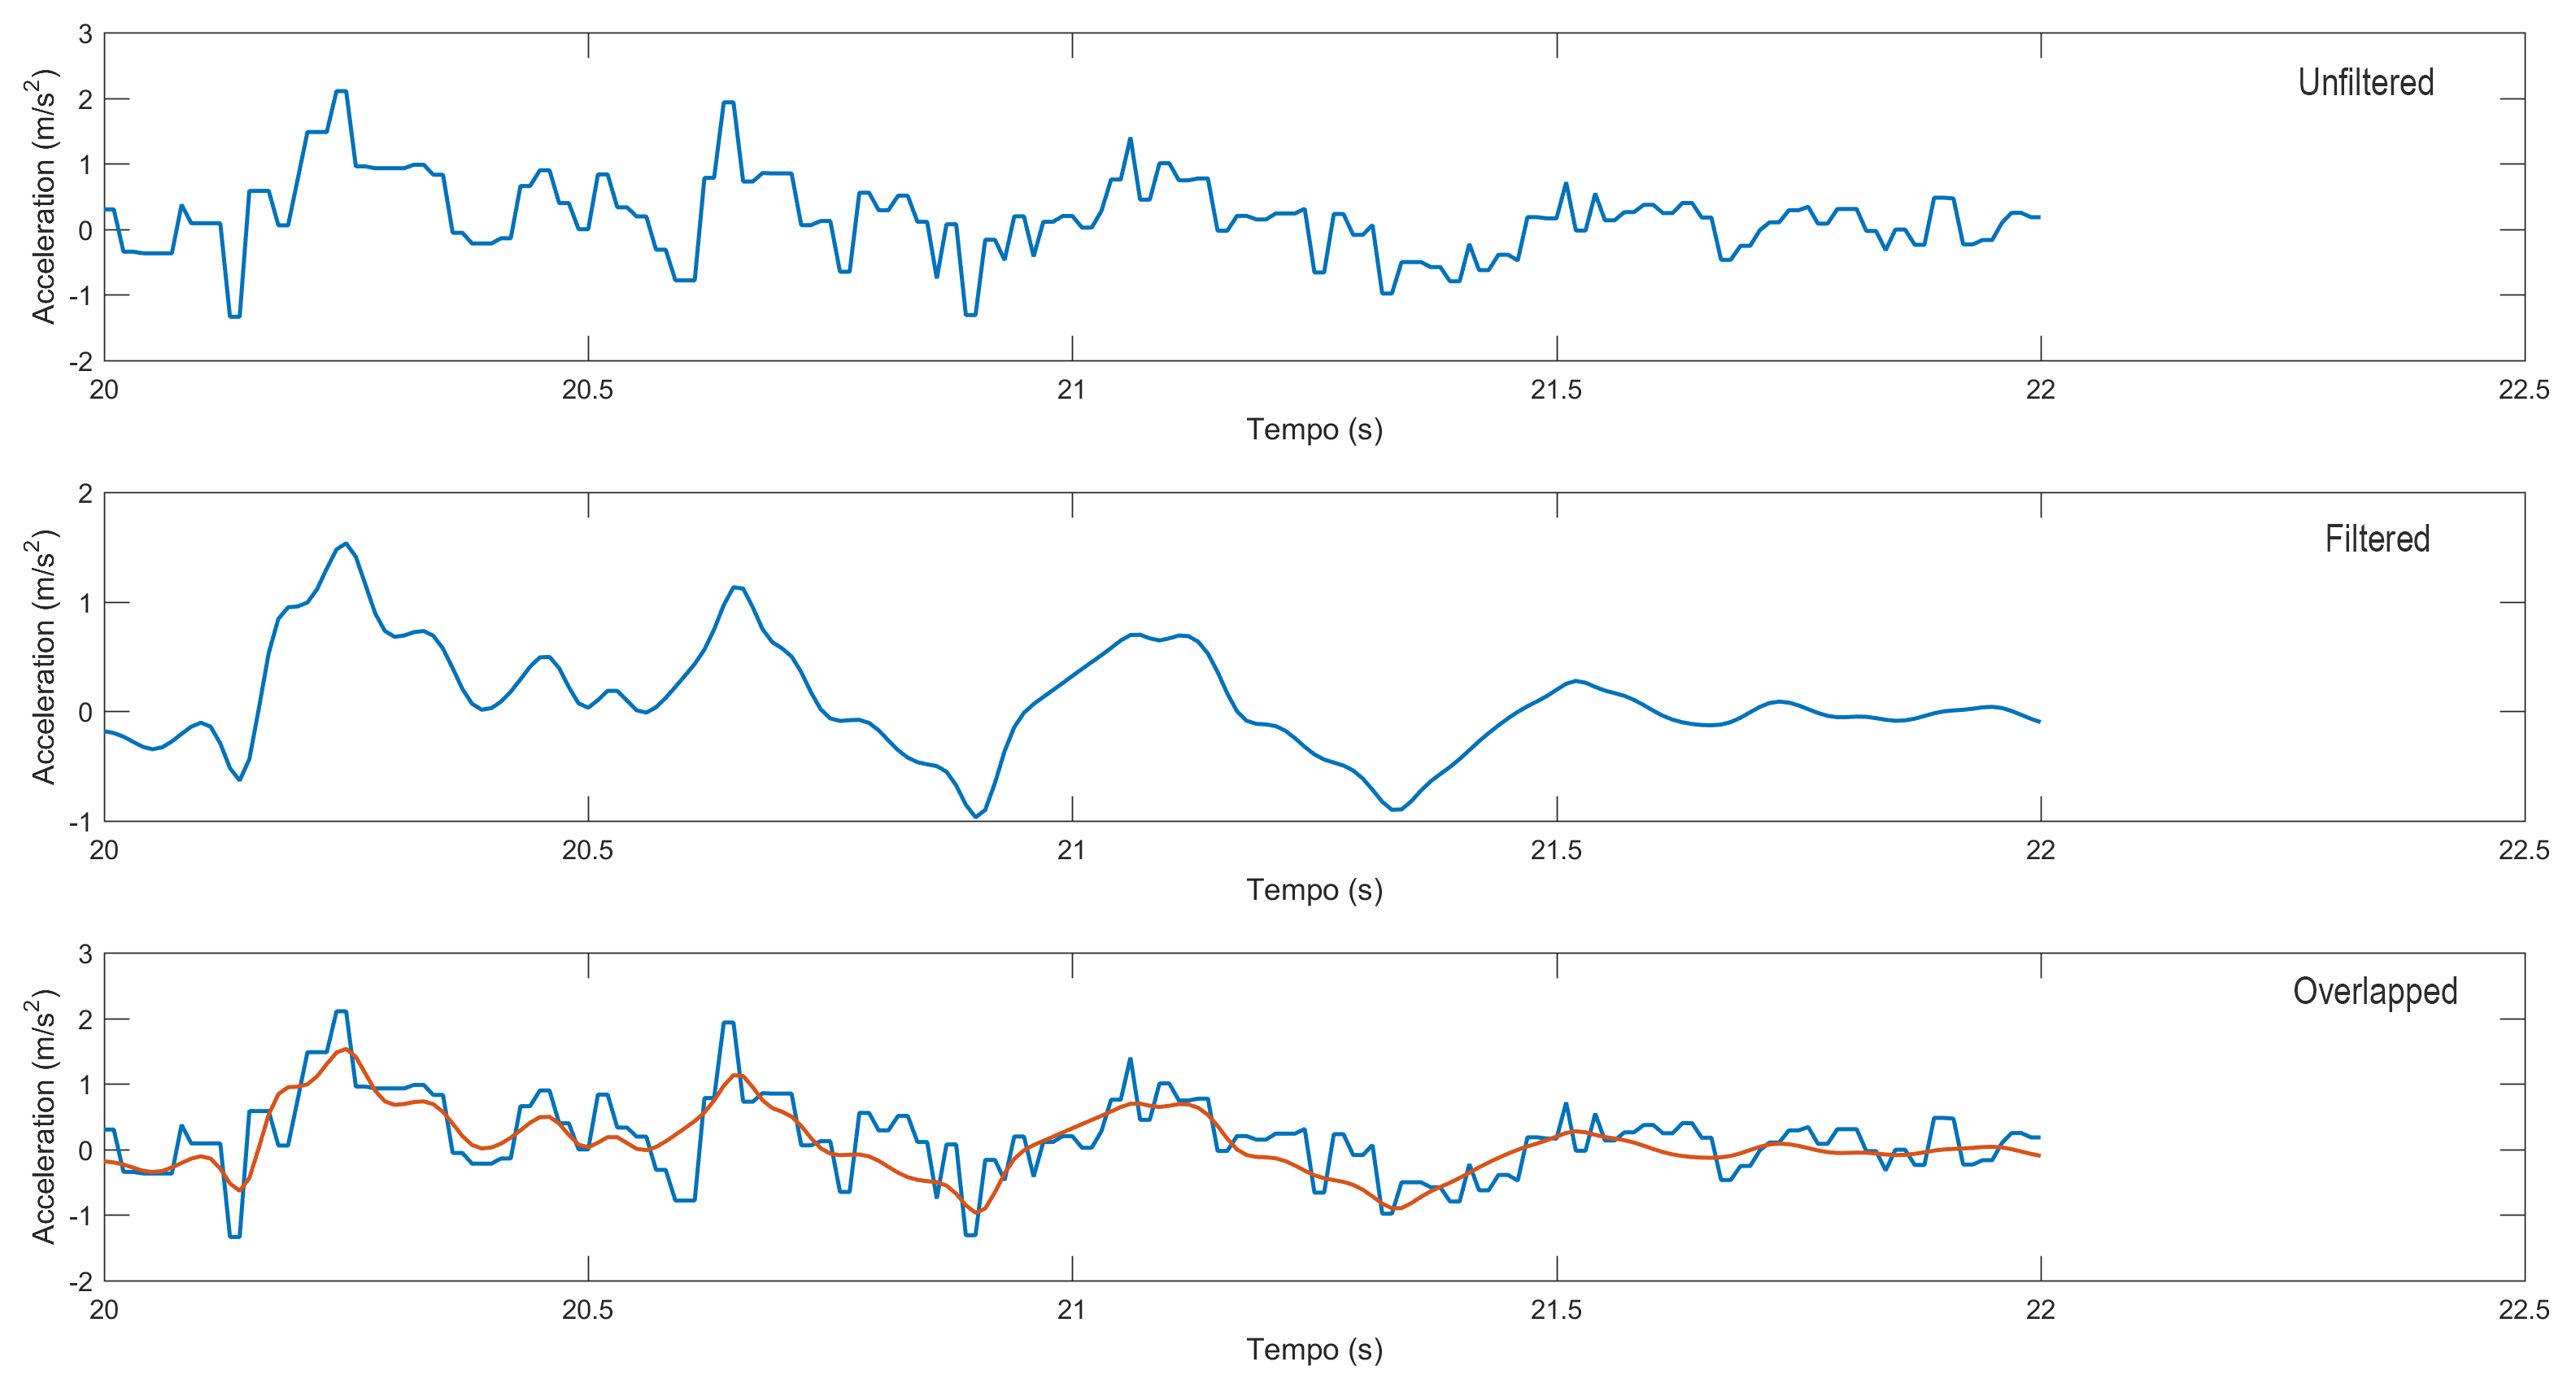
\includegraphics[scale=0.15]{IRIDetailedFiltering}
\caption{Original Signal (blue) compared with the filter Signal (orange) relative to a little set of data}
\end{figure}
As it is possible to see, the signal now is lighter and significantly smoothed, because DC components were been eliminated and background noise has been reduced.
\item[7. Integration of Acceleration, and filtering velocity signal:] After the filtering, the integration of acceleration signal respect to the time(\ref{eq:velocity}) can be performed to obtain the speed. For this purpose, the trapezoidal integration method(\ref{eq:trapezoidal}) was used. Subsequently, the resulting signal will be subject, for the same reasons as discussed in step 6, to the same filtering operations. Because during the acceleration integration, the resulting velocity signal will present DC components to be eliminated.
The result of integration and filtering is shown on the figure:
\begin{figure}[H]
\centering
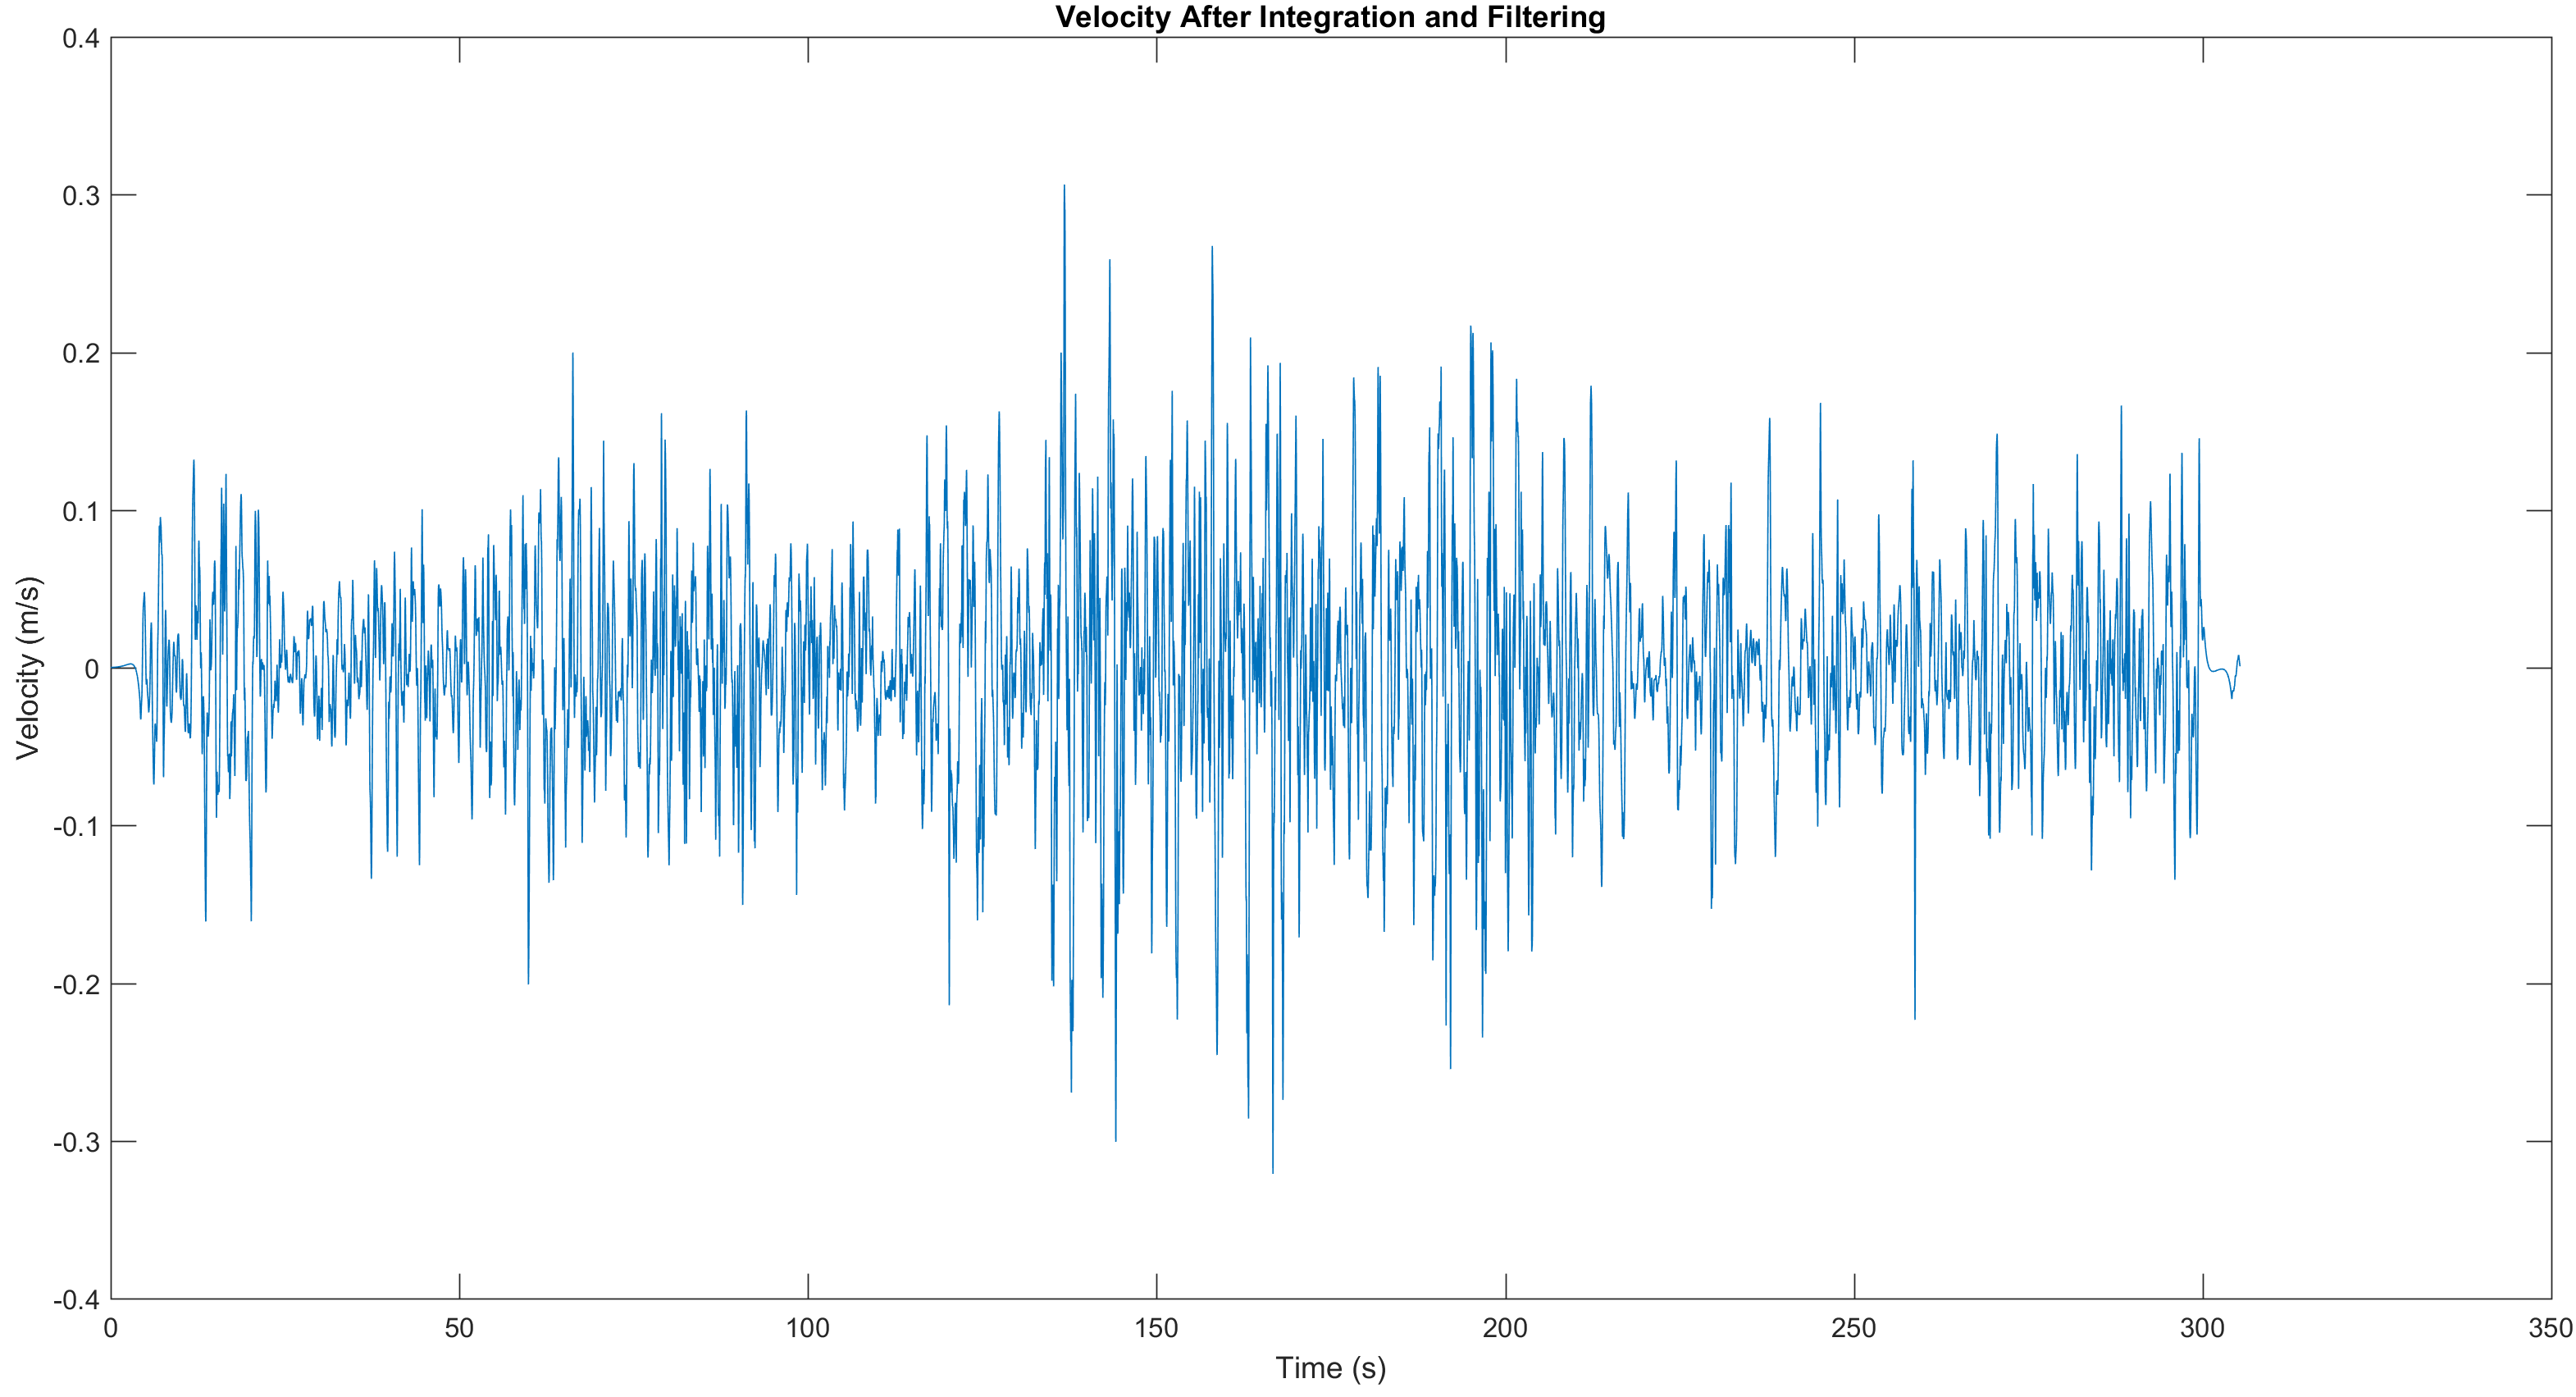
\includegraphics[scale=0.15]{IRIVelocityIntegration}
\caption{Velocity obtained after integration and filtering}
\end{figure}
\clearpage
\item[8. Velocity Integration:]
At this point, the integration of the velocity signal respect to the time(\ref{eq:displacement}) can be performed to obtain the displacement. Also, in this case, the trapezoidal integration method(\ref{eq:trapezoidal}) has been used.

The result of integration is shown on the figure:

\begin{figure}[H]
\centering
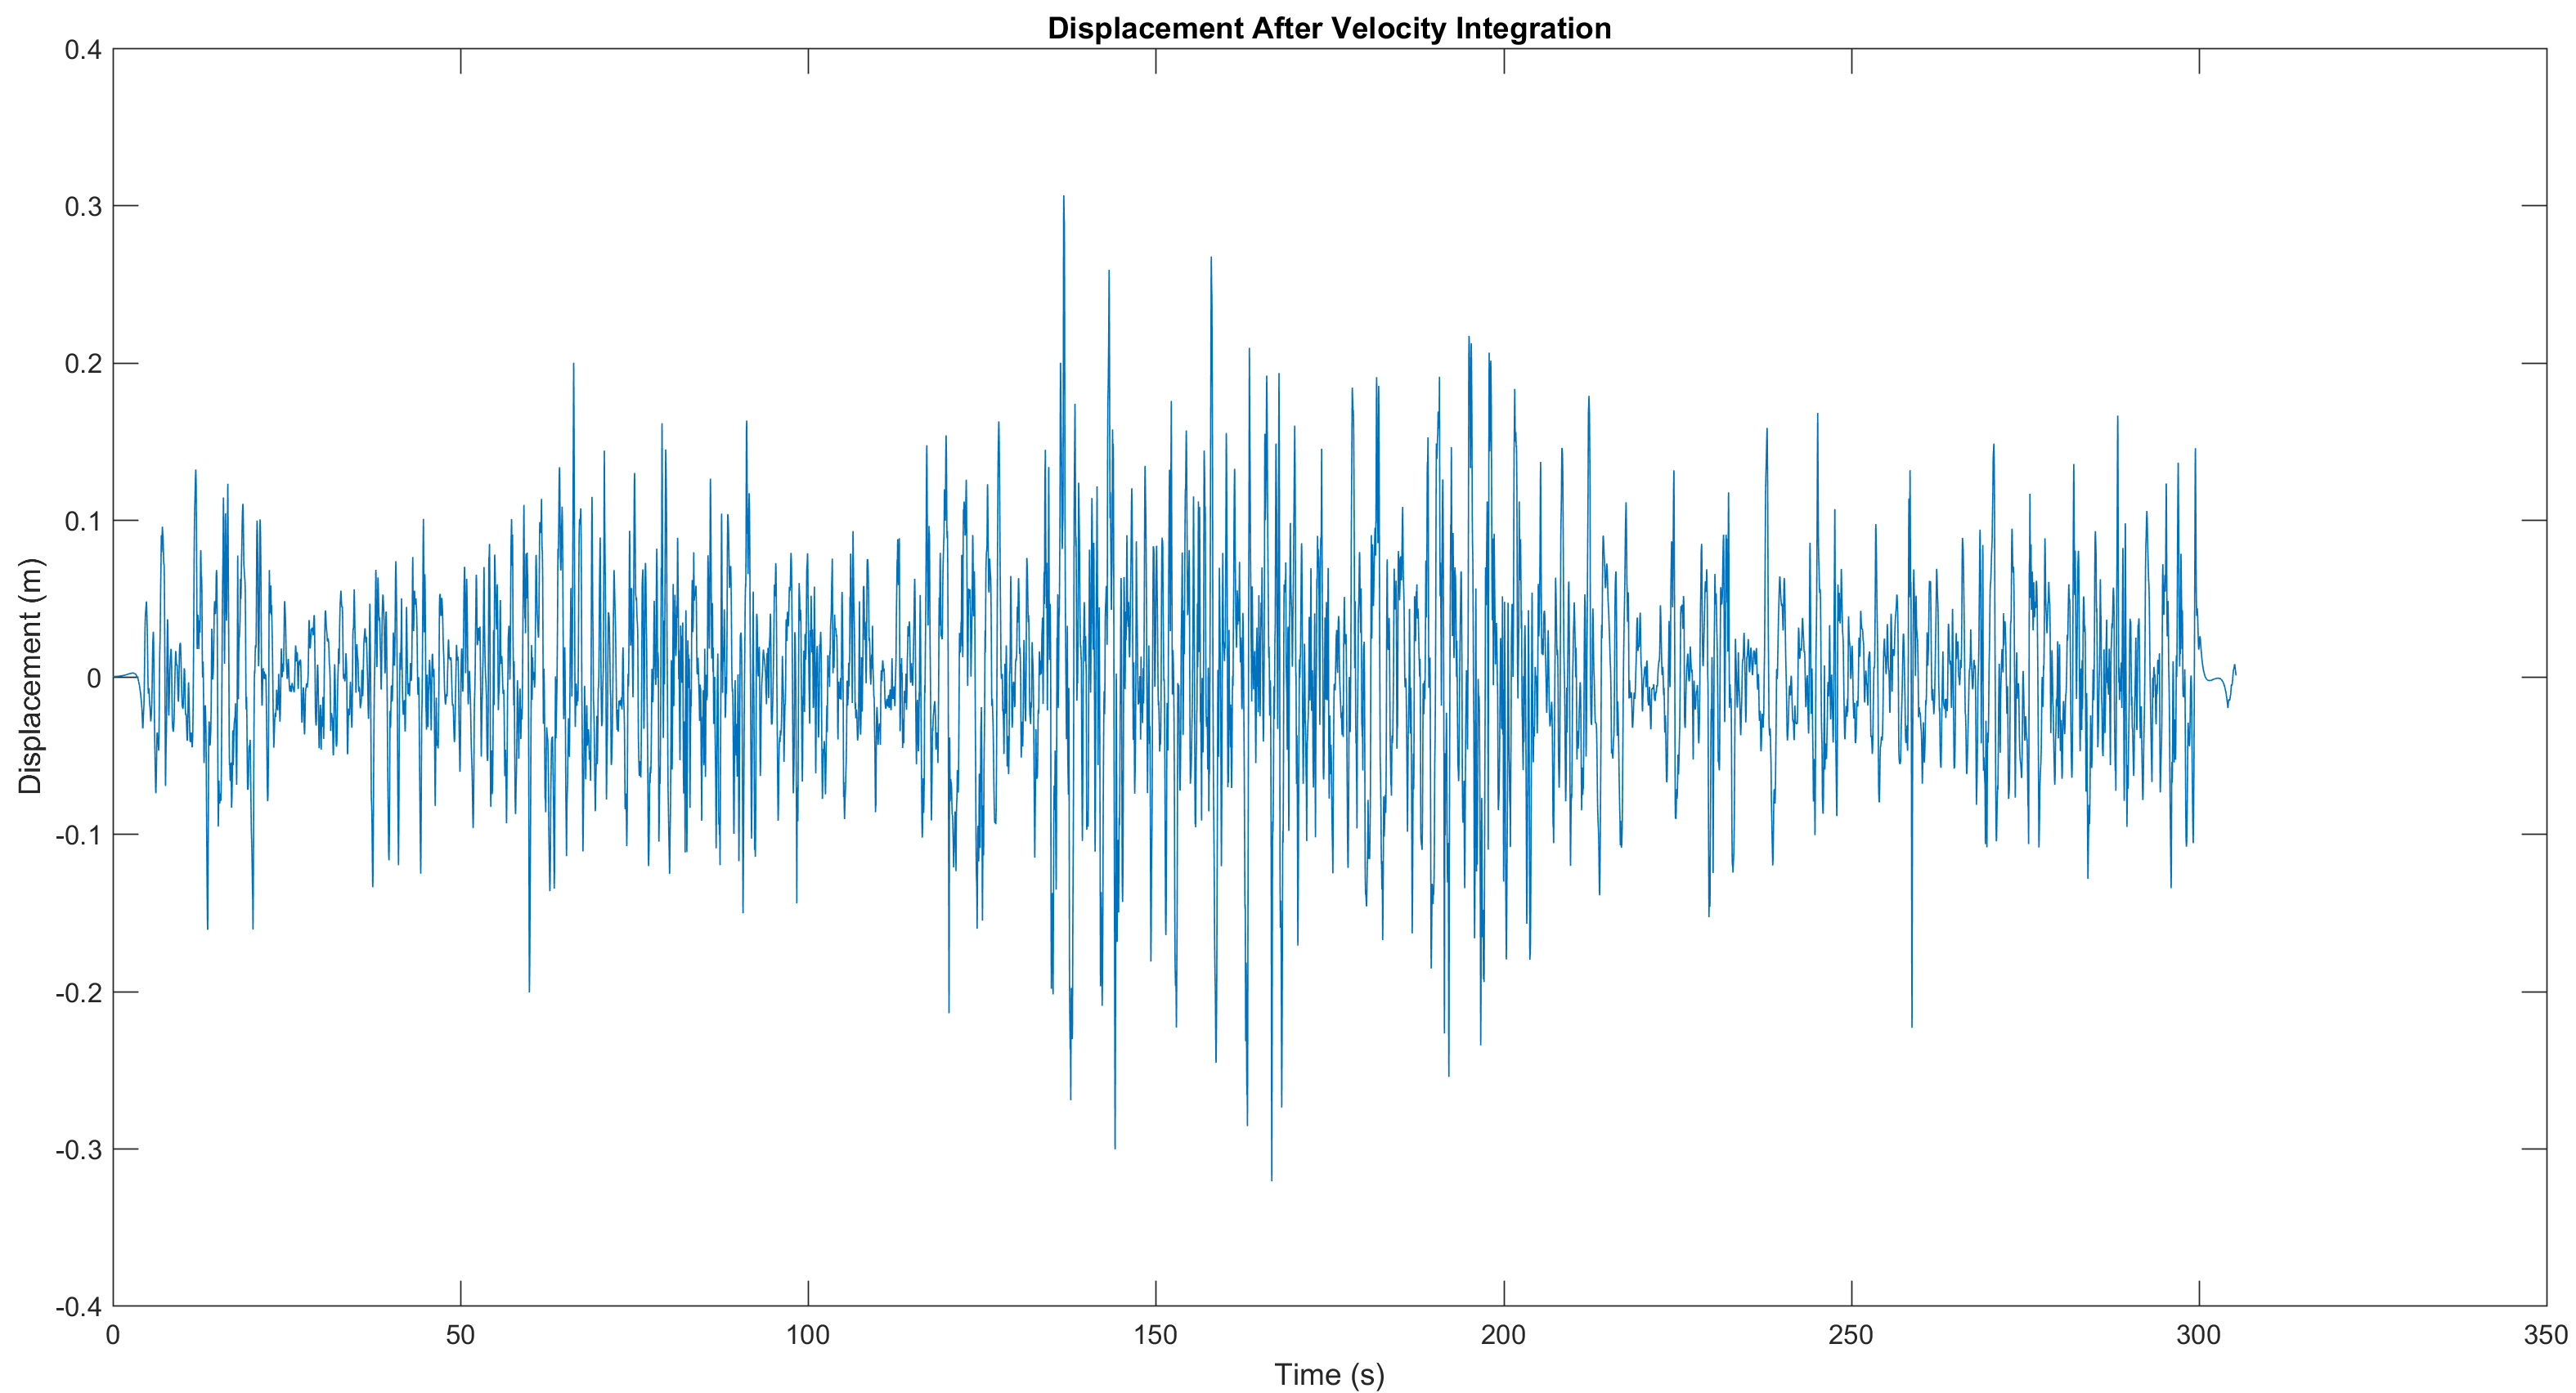
\includegraphics[scale=0.15]{IRIDisplacementIntegration}
\caption{Displacement obtained after velocity integration}
\end{figure}
\item[9. Grouping points in specific distances:] Similarly to the other indexes, even, in this case, the displacement points will have to refer each other to a predetermined distance.
But, since these data will be processed again to derive an IRI estimate.
As indicated \ref{sc:Calculation of IRI}, it is needed a very small segments in order to allow a better accuracy of the result, so the distance between the points, in this case, will be very small.

\begin{figure}[H]
\centering
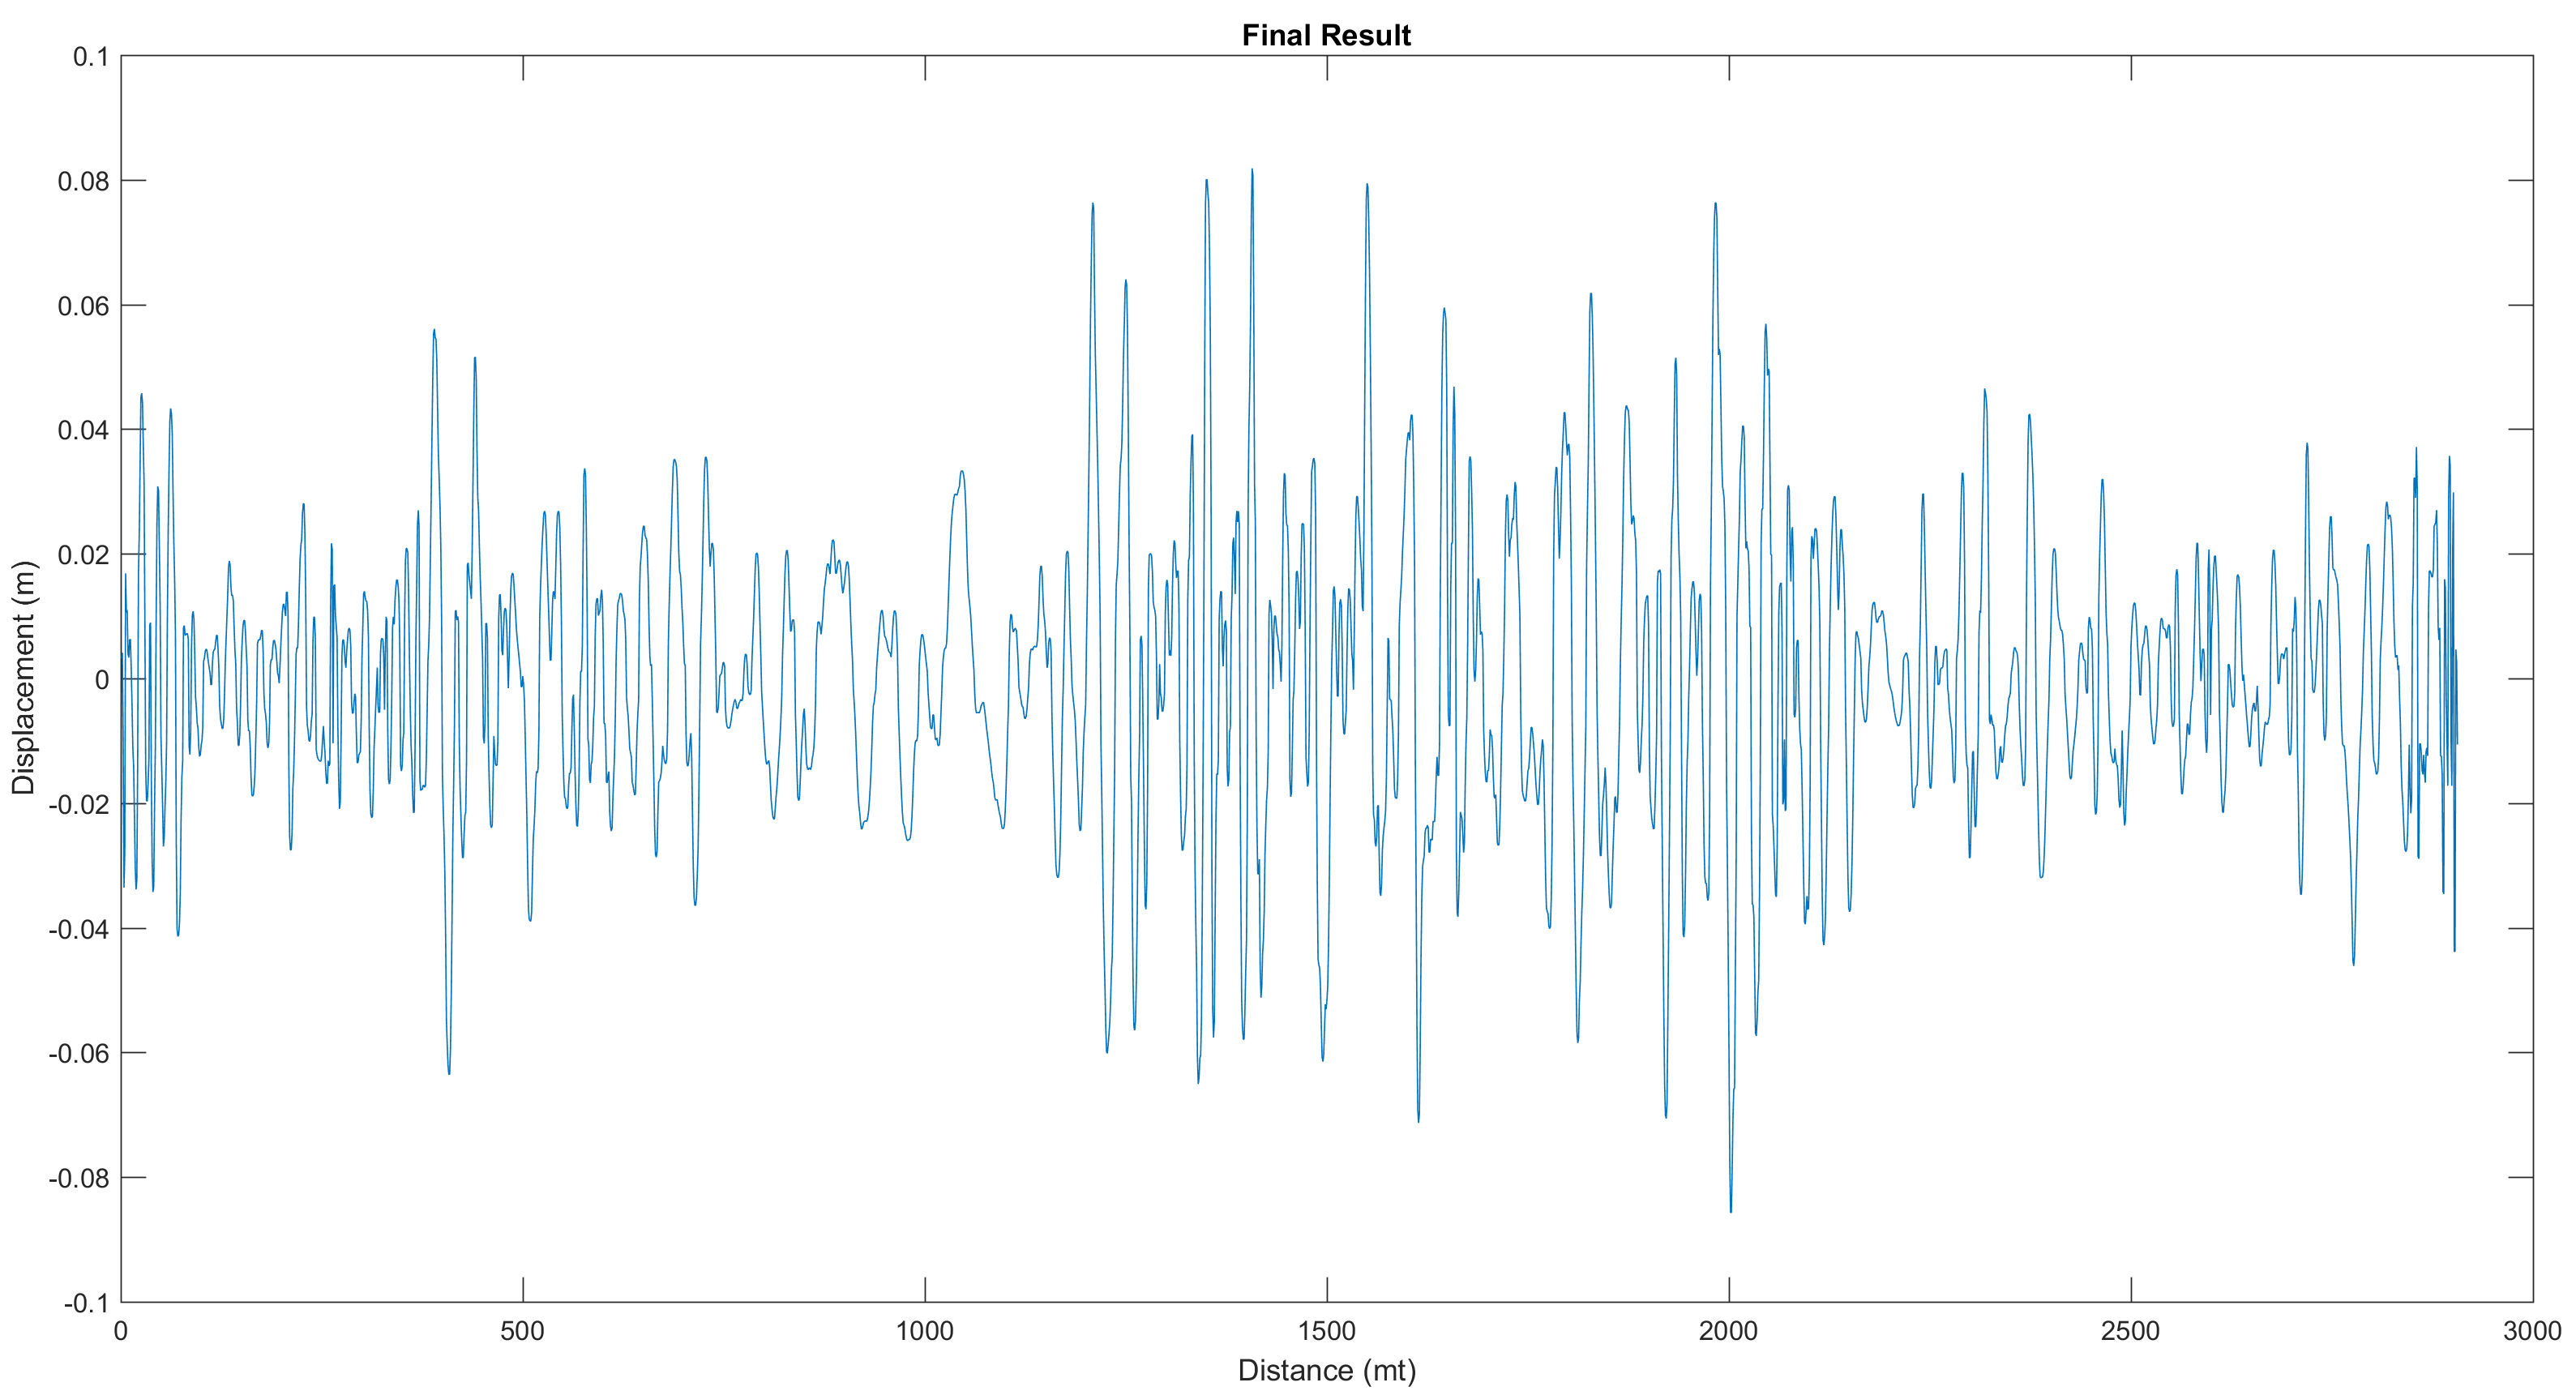
\includegraphics[scale=0.15]{IRIFinalResultAfterGPSDivision}
\caption{Final displacement after grouping points}
\end{figure}

\end{description}


\subsubsection{Calculation of IRI from obtained displacement data}
The resulting displacement data will be processed inside ProVal (Profile Viewing and AnaLysis) software to obtain an IRI\ref{ch:IRI} estimate through a simulation of the quarter car model\ref{ssc:Quarter Car Model}.
Using Class3 instruments, the value must be calculated for every $100$ $\si{\meter}\thinspace +$ of the road(\ref{ssc:correlation}).
Inside ProVal, IRI can be calculated in various ways by performing a ride quality analysis:
\begin{description}
\item[Overall:] Overall calculated on the data series.
\item[Continuos:] An IRI threshold is indicated and road sections above this threshold are identified.
\item[Fixed Interval:] Calculated on fixed interval road	 segments.
\end{description}
In our case, it will be calculated on fixed interval which is of $100$ $\si{\meter}$.

Imported the data, the computation will be done by simulating the quarter car model(\ref{ssc:Quarter Car Model}) and applying the IRI Filter(\ref{sc:Calculation of IRI})
Below is shown an example of the IRI computation of a data series.
\begin{figure}[H]
\centering
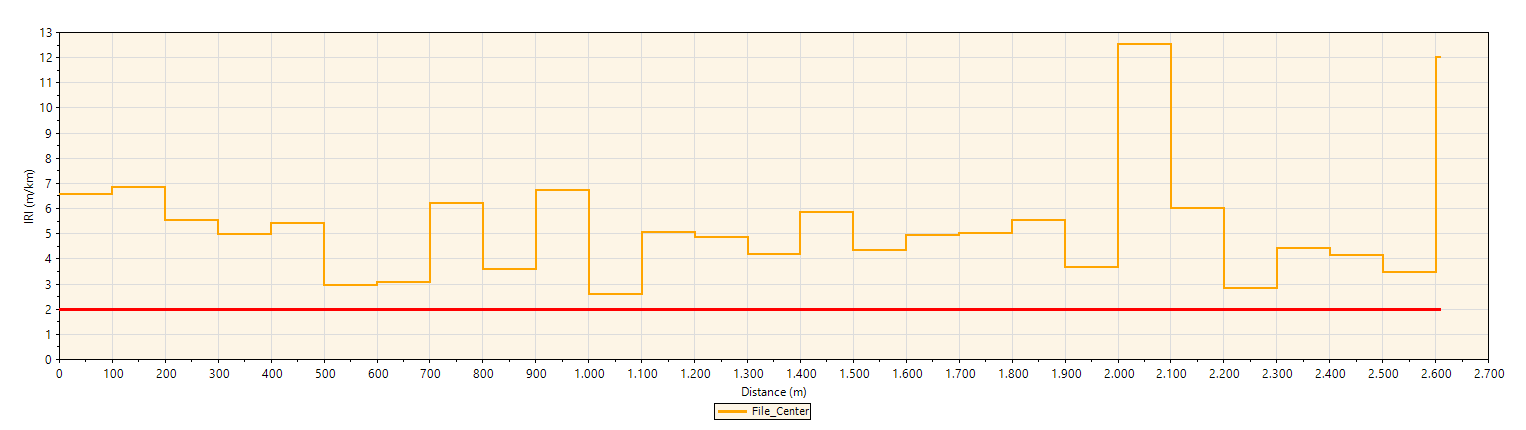
\includegraphics[scale=0.35]{IRI_PROVAL}
\caption{IRI computation result}
\end{figure}\label{fig:IRI computation result}


\subsubsection{Correlation phase}
For these measurement systems, a correlation equation\ref{ssc:correlation} that can be derived from a Class1 or Class2 instruments it is needed, but because we do not own any of them, it has only been simulated.

\clearpage
\section{Data Storing}\label{sc:data_storing}
After the processing is ended, the results of the respective indexes will be saved on a database by using a Java application where a connection to a MySql database is established using the MySql Connector.
For each point of the index in question, they will be stored:
\begin{itemize}
\item \textbf{Value}
\item \textbf{GPS coordinates:} in terms of Latitude and Longitude.
\item \textbf{Registration Date}
\item \textbf{Point Color}
\end{itemize}
In the previous chapter\ref{ch:System Development}, we have seen that each point on the other is separated by a $distance_{fixed}$ called $ds$. However, it may happen that some points are close to each other, because if you suppose that the recording is related to road paths that are run on both lanes, some points may be overlap between them or in any case be very close, because of the GPS accuracy (within $10$ m) in wich the data are stored. A check on the processed data set will be carried out to examine if there are points close to each other within a distance of:

\begin{center}
$\dfrac{ds}{2}$,
\end{center}

if this happens, a single point will be extracted.
Additionally, to each point, a color will be assigned using the HSV color space. This depending on the type of index in question and the value attributed to the point. Generally, a color ranging goes from green (optimal conditions) to red (critical conditions).

To make the read and save faster and more efficacious, a pool of connections was used, in which various threads perform operations on the database. With regard to the insert/update phase, because the data will often refer to the same road sections, it need be checked in this case before insertion, if a point already intersects with a segment referring to points previously saved. If this happens it will be associated with the nearest edge and the value is identified as the average of the two, only updating the point already in the database. Otherwise, if this does not happen a new point is inserted.


\clearpage
\section{Viewing on interactive map}\label{sc:Viewing on interactive map}
Finally, processed data will be displayed on an interactive map using the Open Source Mapbox Map. A website for points representation has been developed, in wich, each of these is represented by specific color circle using Mapbox APIs.

The density of the points is high. It is, therefore, necessary to have a system capable of clustering them, depending on the zoom of the map display, in fact, if the zoom was low, the points are grouped into larger circles, vice versa if the zoom increases circles they expand until they reaching their atomic dimension.
The figures below show the start page of the site and an example of the circle clustering associated with the minimum and maximum zoom level.

\begin{figure}[H]
\centering
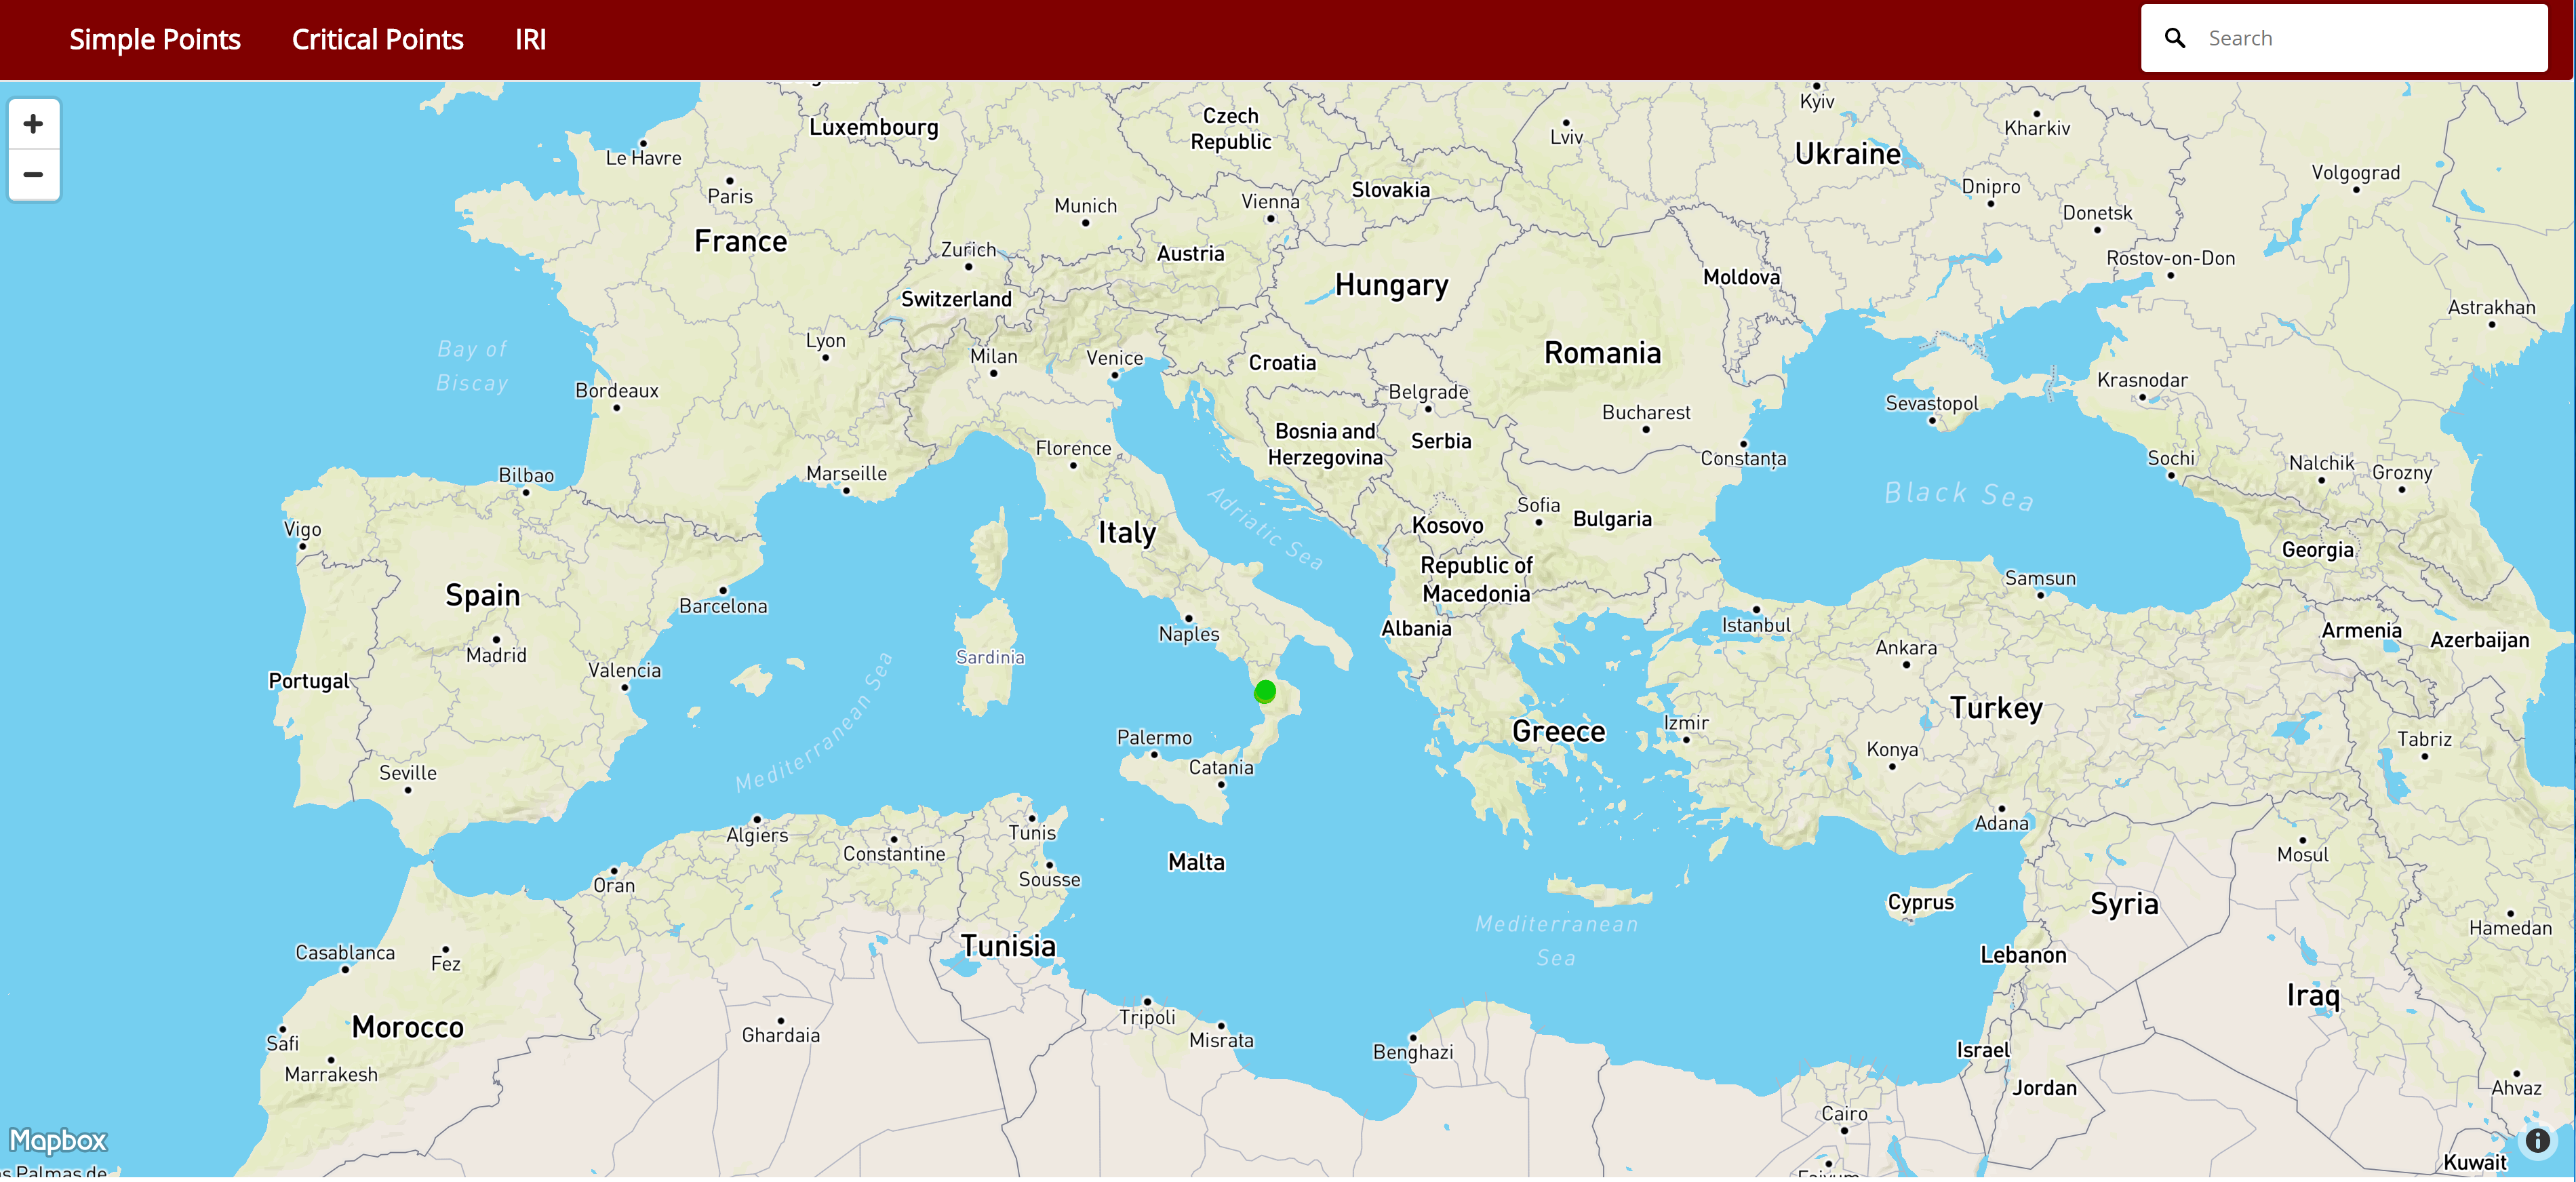
\includegraphics[scale=0.4]{MainPage}
\caption{Web Site main page}
\end{figure}\label{fig:WebSite Main Page}

\begin{figure}[H]
  \centering

  \subfloat[Min Zoom Level]{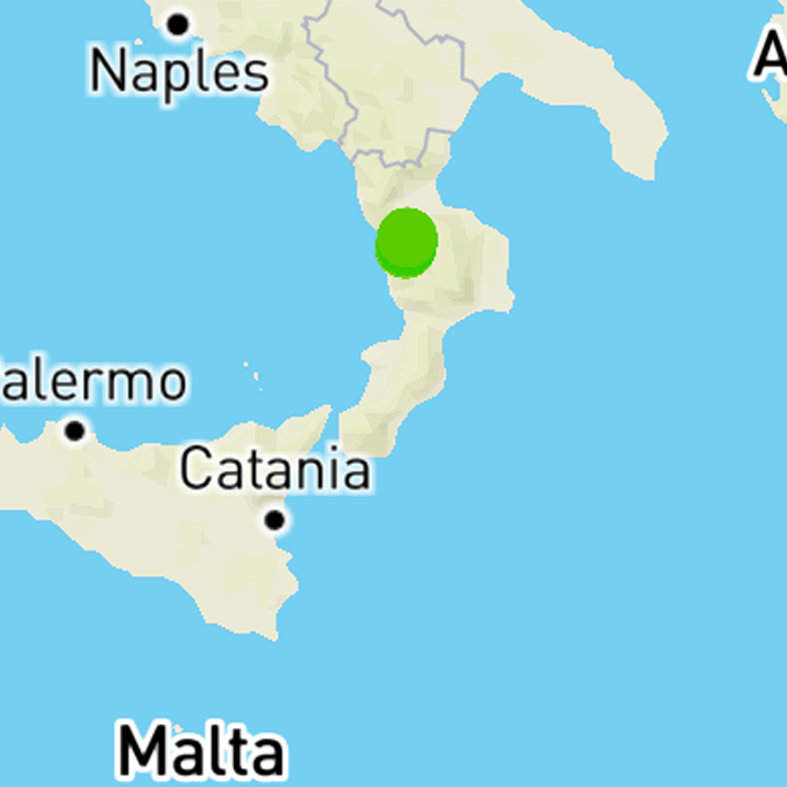
\includegraphics[scale=0.6]{MinZoom}}\hspace{10mm}
  \subfloat[Max Zoom Level]{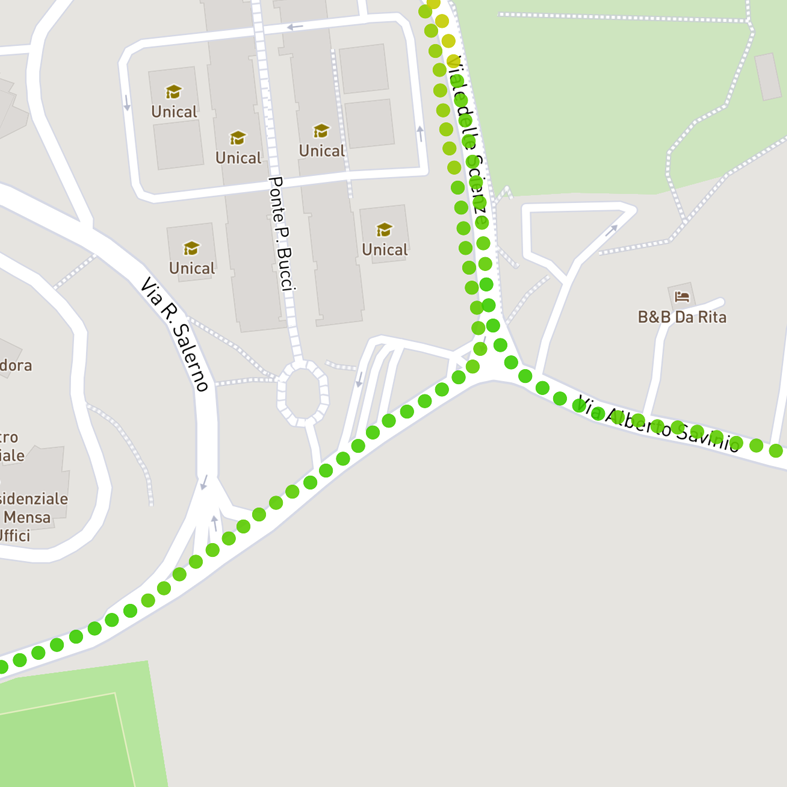
\includegraphics[scale=0.6]{MaxZoom}}
  \caption{Point Clustering based on Zoom Level}
  \label{fig:Point Clustering based on Zoom Level}
\end{figure}
\clearpage


As can be seen in the figure:\ref{fig:WebSite Main Page}, from the navigation bar it is possible to choose which index will be displayed by clicking on the corresponding button. When is decided to change view by clicking on one of them, an AJAX request will be sent to a Servlet, which queries the database to get the points of the required index, the result is inserted in the AJAX response, from which the GEOJSON (a format for the encoding of different geographic structures) will be created, which will be associated with the map to change the representation layer without reloading the page.
It is also possible to search for specific locations from the search bar on the main navigation bar.
The specific information of each point is obtainable by clicking on it, where a pop-up is opened, and it shows the registration date and the value associated with that index.

The figure below shows the example of a pop-up.


\begin{figure}[H]
\centering
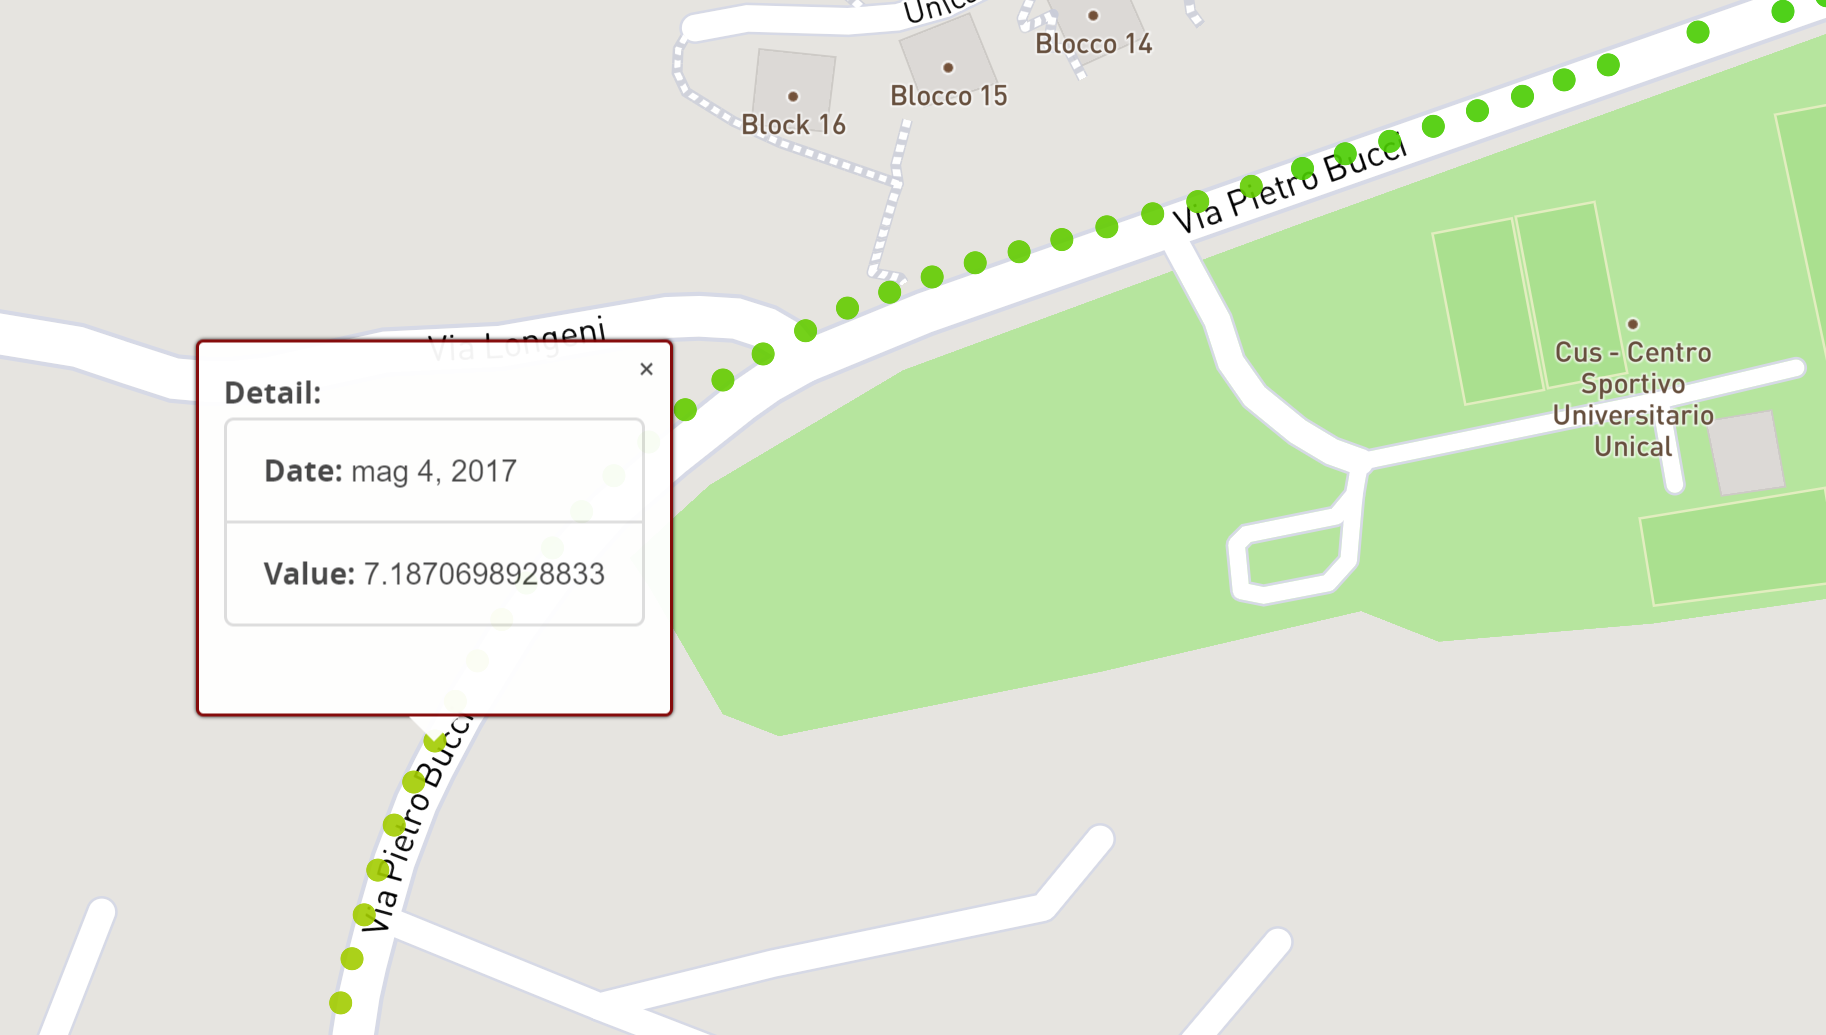
\includegraphics[scale=0.7]{PopUp}
\caption{Example of PopUp}
\end{figure}\label{fig:PopUp}
\end{document}